\chapter{Concatenated backward ray mapping}\label{chap:raymapping1}
In the previous chapter we have seen that PS ray tracing based on the source and the target PS constitutes an improvement of MC and QMC ray tracing. 
Now, a method that employs not only the source and the target PS but also the PS of \textit{all} the other lines that constitute the optical system is introduced. 
% Furthermore, instead of starting from the source, the new approach is an inverse method which starts considering rays on target PS.
In this chapter, we consider systems formed only by straight and reflective line segments.
All lines can be modeled as receivers of the incident light and emitters of the reflected light, they constitute
the target for incident rays and the source for reflected rays.
Moreover, we assume that the source can only emit light and the target can only receive light.
%Therefore, 
%one PS is taken into account for the source and one for the target while both the source and target phase spaces are considered for the other lines. E%
%Every line of the system (except for the source \point{S} and the target \point{T}) . 
Therefore, two different PS are considered for the reflectors and one PS for
\point{S} and \point{T}. All these phase spaces are connected through a map which relates the ray coordinates on every PS. This map can be written as the concatenation of many maps which can be classified as two different kind of maps, i.e., the map that connects the source and the target PS of two \textit{different} lines and the map that connects the target and the source PS of the \textit{same} line.
Employing the inverses of these maps we are able to detect the parts of target PS illuminated by the source.
All the PS considered are divided into several regions, the boundaries of which can be determined exactly for systems formed by straight lines.
We make the assumption of a Lambertian source.
%; hence, the luminance is a positive constant inside a when different from $0$. 
As a consequence, the output intensity along a given direction is obtained from the total width of all the patches with positive luminance, measured along that direction.\\ \indent 
%In this chapter we explain the method for systems formed by straight and reflective lines segment. 
In this chapter, two different optical systems are investigated: the two-faceted cup and the so-called multi-faceted cup. Next, the details of the procedure are explained for the two-faceted-cup.
\section{Phase spaces of the two-faceted cup}\label{sec:cup_raymapping}
A two-faceted cup is introduced in Chapter \ref{chap:raytracing} and depicted in Figure \ref{fig:cup}. It is formed by a source \point{S}, a target \point{T} and two reflectors which are straight lines segments. 
Using the same notation of Chapter \ref{chap:PS}, we denote with $\mbox{\set{S}{}{}}=\mbox{\set{Q}{}{}}\times\mbox{\set{P}{}{}}$ the PS and with 
$(\variabile{q}, \variabile{p})$ the rays coordinates in \set{S}{}{}.\\ \indent
Let's now introduce some new notation. 
The source and the target PS of a line $\lineai$ are indicated with \set{S}{\lineai}{} and \set{T}{\lineai}{}, respectively. The initial rays coordinates in \set{S}{}{} are denoted with $(\pos{s,}{$1$}, \dir{s,}{$1$})$.
The coordinates of every ray that reaches the line $\lineai\in\{2, 3, 4\}$ are indicated  with $(\pos{t,}{\lineai}, \dir{t,}{\lineai})$ on \set{T}{\lineai}{}. 
In the following, to simplify the notation, we indicate the target coordinates of the rays on \set{T}{$4$}{} with (\variabile{q}, \variabile{p}) instead of $(\pos{t,}{$4$}, \dir{t,}{$4$})$.
After reflection, the ray leaves line $\lineai \in\{2, 3\}$ at the same position but with a different direction, the new ray coordinates are indicated with 
$(\pos{s,}{\lineai}, \dir{s,}{\lineai})$ on \set{S}{\lineai}{}. 
Note that $\pos{s,}{\lineai}= \pos{t,}{\lineai}$, while $\dir{s,}{\lineai}$ is obtained applying the reflection law to the direction coordinate $\dir{t,}{\lineai}$ of the incident ray.

The phase spaces \set{S}{\lineai}{} and  \set{T}{\lineai}{} of each line $\lineai$ are partitioned into different regions, (\set{S}{\lineai,}{\lineaj})$_{\lineaj=2, 3, 4}$ and (\set{T}{\lineai,}{\lineak})$_{\lineak=1, 2, 3}$, respectively, where $\lineaj\neq \lineai$ is the index of the line that is illuminated by $\lineai$ and $\lineak\neq\lineai$ is the index of the line that illuminates $\lineai$. Hence, \set{S}{\lineai,}{\lineaj}$\subset$ \set{S}{\lineai}{} is the part of \set{S}{\lineai}{} corresponding to rays that illuminate line $\lineaj$, and \set{T}{\lineai,}{\lineak} $\subset$ \set{T}{\lineai}{} is the part of \set{T}{\lineai}{} corresponding to rays originating from the line $\lineak$. Note that, due to the fact that the source only emits light, we do not define its target PS \set{T}{$1$}{}. Similarly, since the target only receives light, its source PS \set{S}{$4$}{} is not defined.
For the two-faceted cup, six different phase spaces need to be considered which are given by the following expressions:
\begin{equation}
\label{SPS}
\begin{split}
 \mbox{\set{S}{$1$}{}} & = \mbox{\set{S}{$1$,}{$2$}}\cup
 \mbox{\set{S}{$1$,}{$3$}} \cup \mbox{\set{S}{$1$,}{$4$}},\\
\mbox{\set{S}{$2$}{}} & =  \mbox{\set{S}{$2$,}{$3$}} \cup \mbox{\set{S}{$2$,}{$4$}},\\
\mbox{\set{S}{$3$}{}} & =  \mbox{\set{S}{$3$,}{$2$}} \cup \mbox{\set{S}{$3$,}{$4$}},\\
\mbox{\set{T}{$2$}{}} & = \mbox{\set{T}{$2$,}{$1$}} \cup \mbox{\set{T}{$2$,}{$3$}},\\
\mbox{\set{T}{$3$}{}} & = \mbox{\set{T}{$3$,}{$1$}}\cup \mbox{\set{T}{$3$,}{$2$}},\\
\mbox{\set{T}{$4$}{}} & = \mbox{\set{T}{$4$,}{$1$}}\cup \mbox{\set{T}{$4$,}{$2$}}\cup
\mbox{\set{T}{$4$,}{$3$}}.
\end{split}
 \end{equation}
Note that, as the source cannot receive light and the target cannot emit light,  the regions $(\mbox{\set{S}{\lineai,}{$1$}})_{\lineai=2,3}$ and $(\mbox{\set{T}{\lineai,}{$4$}})_{\lineai=2, 3}$ are not considered. 
\\ \indent The boundaries $\partial \mbox{\set{S}{\lineai,}{\lineaj}}$ are mapped into the boundaries $\partial \mbox{\set{T}{\lineaj,}{\lineai}}$ for every $\lineai=\{1, 2, 3\}$ 
and $\lineaj=\{2, 3,4\}$ with $\lineaj\neq \lineai$ (edge-ray principle). For the two-faceted cup, and for all systems formed by straight line segments, these boundaries can be determined analytically. Given two lines $\lineai$ and $\lineaj$
with $\lineai\neq \lineaj$, the boundaries \set{S}{\lineai}{} and \set{T}{\lineaj}{} are determined as follows. Let $(\variabile{x}_{\lineai, \ell}, \variabile{z}_{\lineai, \ell})$ and $(\variabile{x}_{\lineai, \textrm{r}},\variabile{z}_{\lineai, \textrm{r}})$ be the coordinates of the points located at the left and the right extreme of line $\lineai$, respectively.
Similarly, $(\variabile{x}_{\lineaj, \ell}, \variabile{z}_{\lineaj, \ell})$ and $(\variabile{x}_{\lineaj, \textrm{r}},\variabile{z}_{\lineaj, \textrm{r}})$ are the coordinates of the points located at the left and the right extreme of line $\lineaj$, respectively.
The boundaries $\partial$\set{S}{\lineai,}{\lineak} and $\partial$\set{T}{\lineak,}{\lineai} are  %obtained considering all the rays that leave the end points of line $\lineai$ 
%and all the rays that reach the end points of $\lineaj$.
formed by four different curves,
two of them are given by all the rays that leave the end points of line $\lineai$ and hit line $\lineak$ and, the others two are given by the rays
that leave the interior of line $\lineai$ and hit the end points of line $\lineak$.
They are given by:
 \begin{equation}
\label{eq:analytic_boundaries}
 \begin{split}
 \partial\mbox{\set{S}{\lineai,}{\lineak}} & = \partial\mbox{\setbound{S}{\lineai,}{\lineak}{\,1}}\cup \partial\mbox{\setbound{S}{\lineai,}{\lineak}{\,2}} \cup \partial\mbox{\setbound{S}{\lineai,}{\lineak}{\,3}}\cup \partial\mbox{\setbound{S}{\lineai,}{\lineak}{\,4}},\\
\partial\mbox{\set{T}{\lineak,}{\lineai}} & = \partial\mbox{\setbound{T}{\lineak,}{\lineai}{\,1}}\cup \partial\mbox{\setbound{T}{\lineak,}{\lineai}{\,2}}\cup \partial\mbox{\setbound{T}{\lineak,}{\lineai}{\,3}}\cup \partial\mbox{\setbound{T}{\lineak,}{\lineai}{\,4}}.
 \end{split}
 \end{equation}
In the following we explain in more details the case for $\variabile{\lineai}=1$ and $\variabile{\lineak}=4$ (see Figure \ref{fig:cups}).
\begin{figure}
\centering
\begin{subfigure}{.48\textwidth}
  \centering
  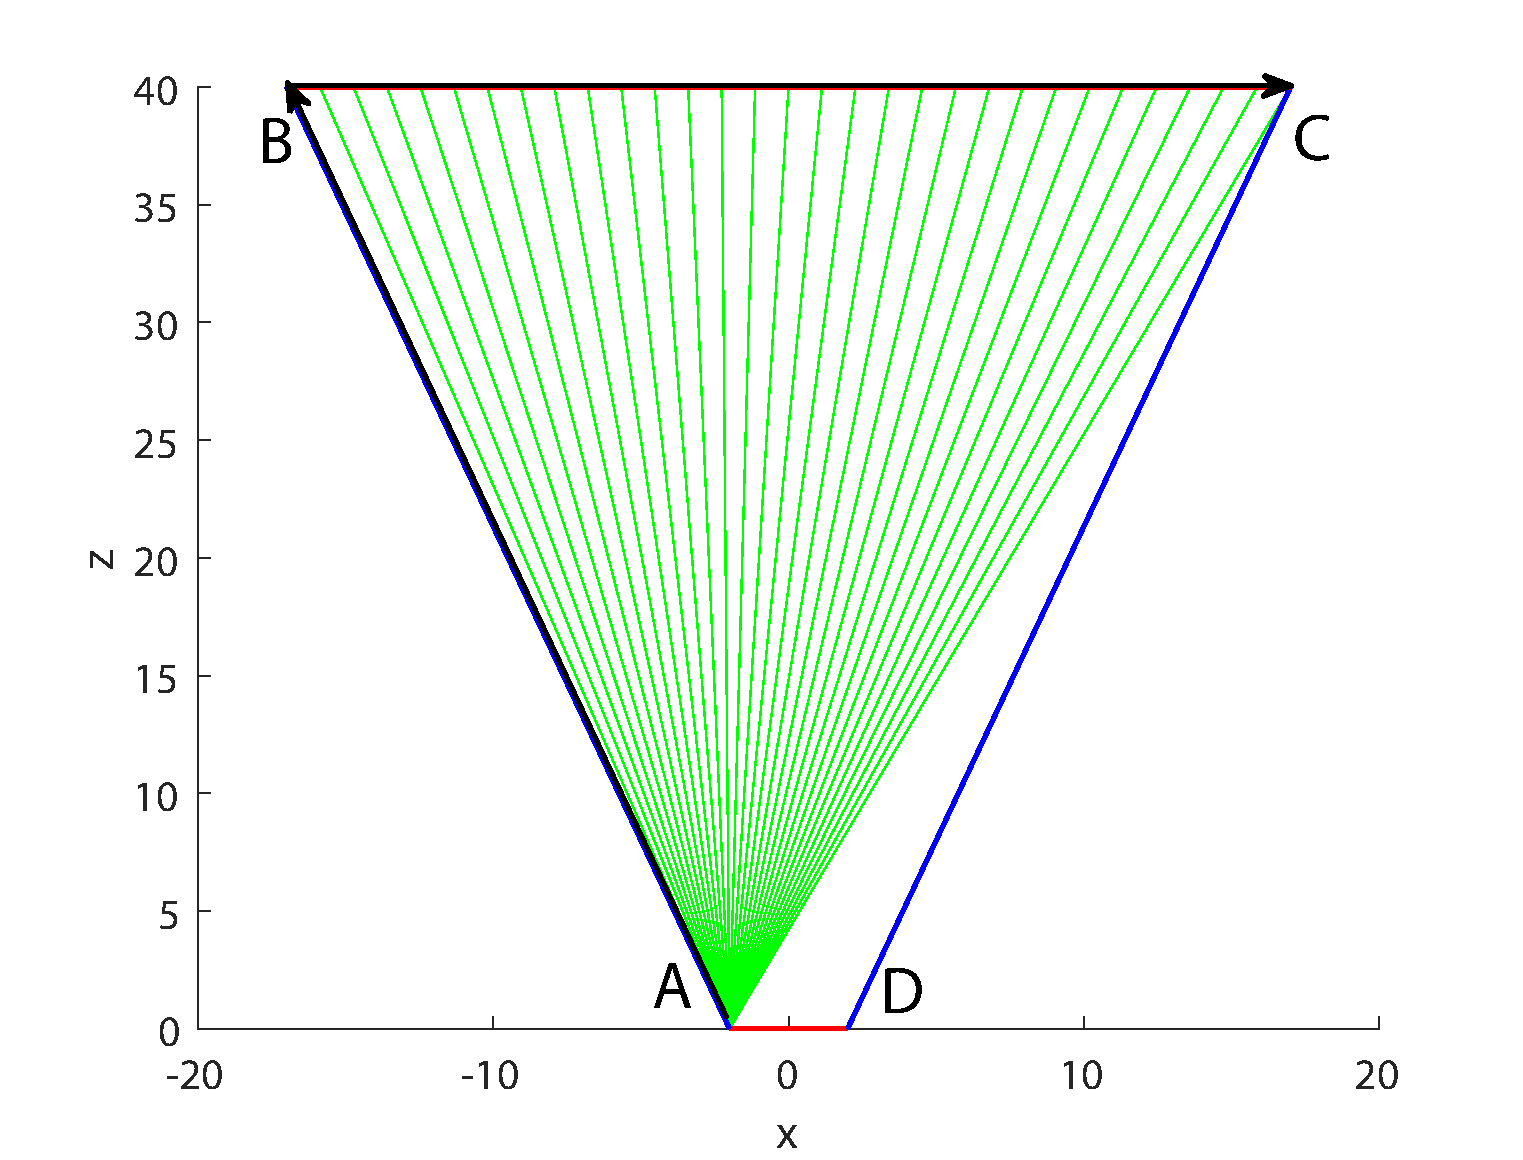
\includegraphics[width=\textwidth]{rays_cup1}
  \caption{Rays that leave the left end point of the source (line $1$) and trace out the target (line $4$).}
  \label{fig:cup1}
\end{subfigure}%
\hfill
\begin{subfigure}{.48\textwidth}
  \centering
  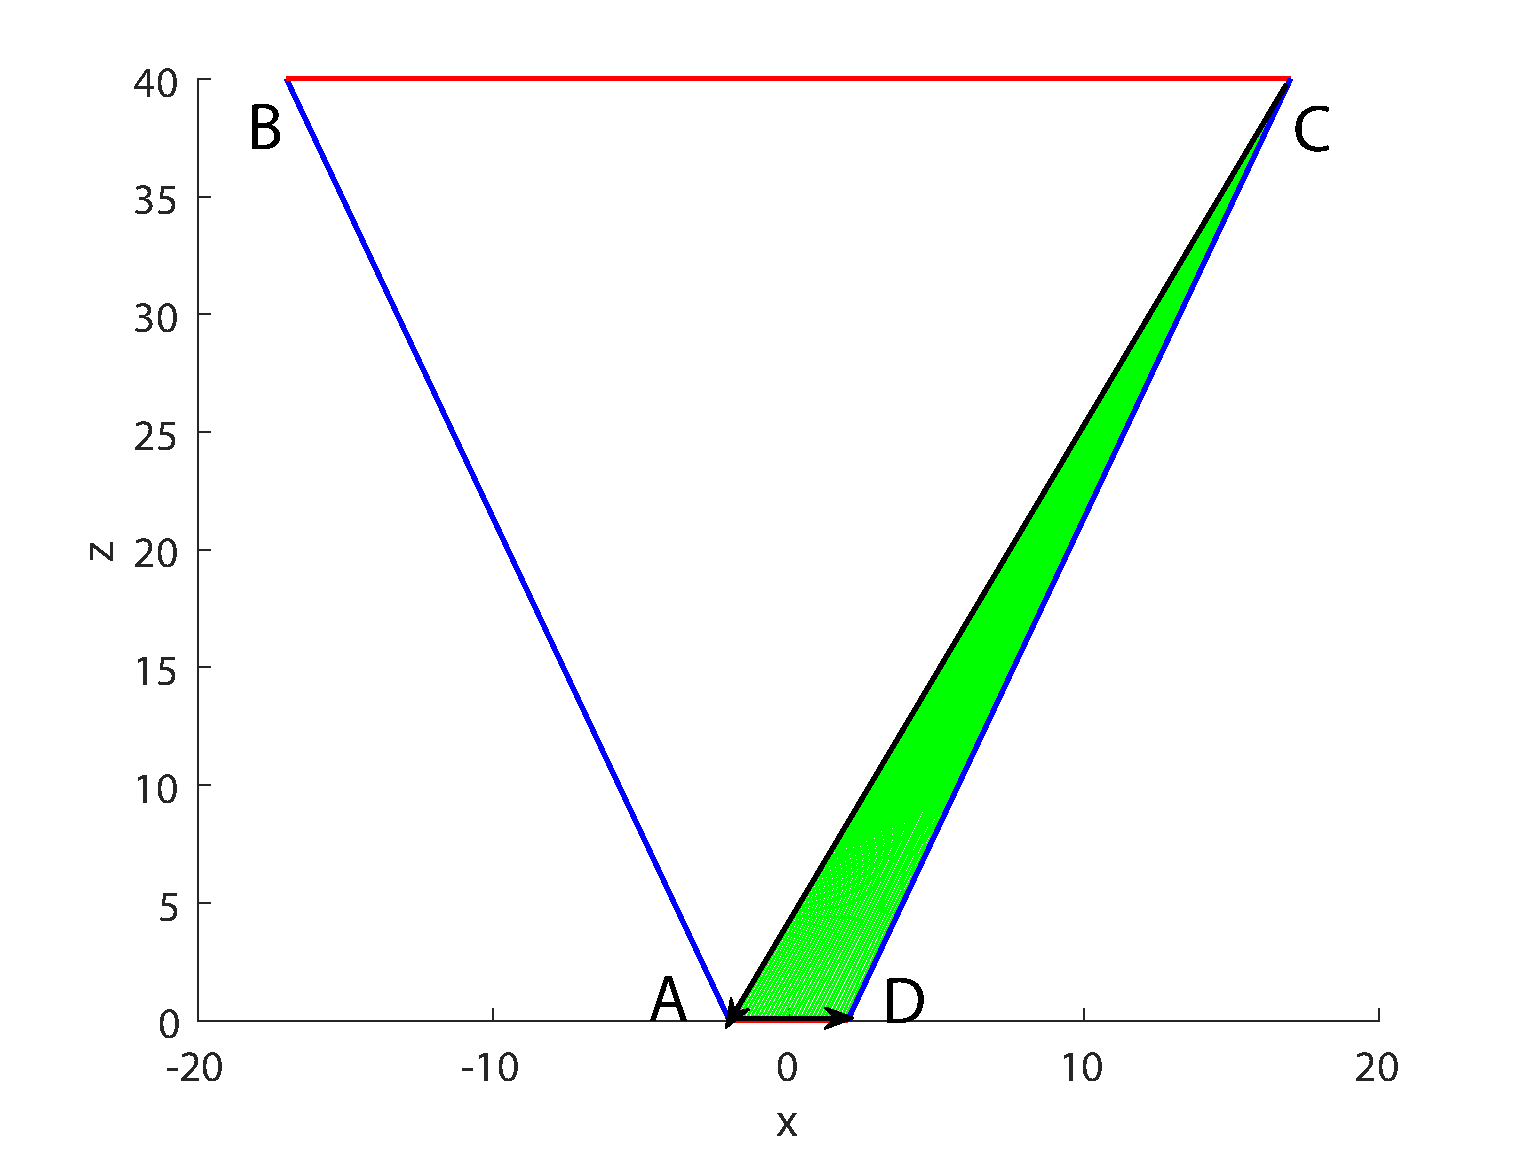
\includegraphics[width=\textwidth]{rays_cup2}
  \caption{Rays that trace out the source (line $1$) and hit the right end point of the target (line $4$).}
  \label{fig:cup2}
\end{subfigure} %
\hfill
\begin{subfigure}{.48\textwidth}
  \centering
  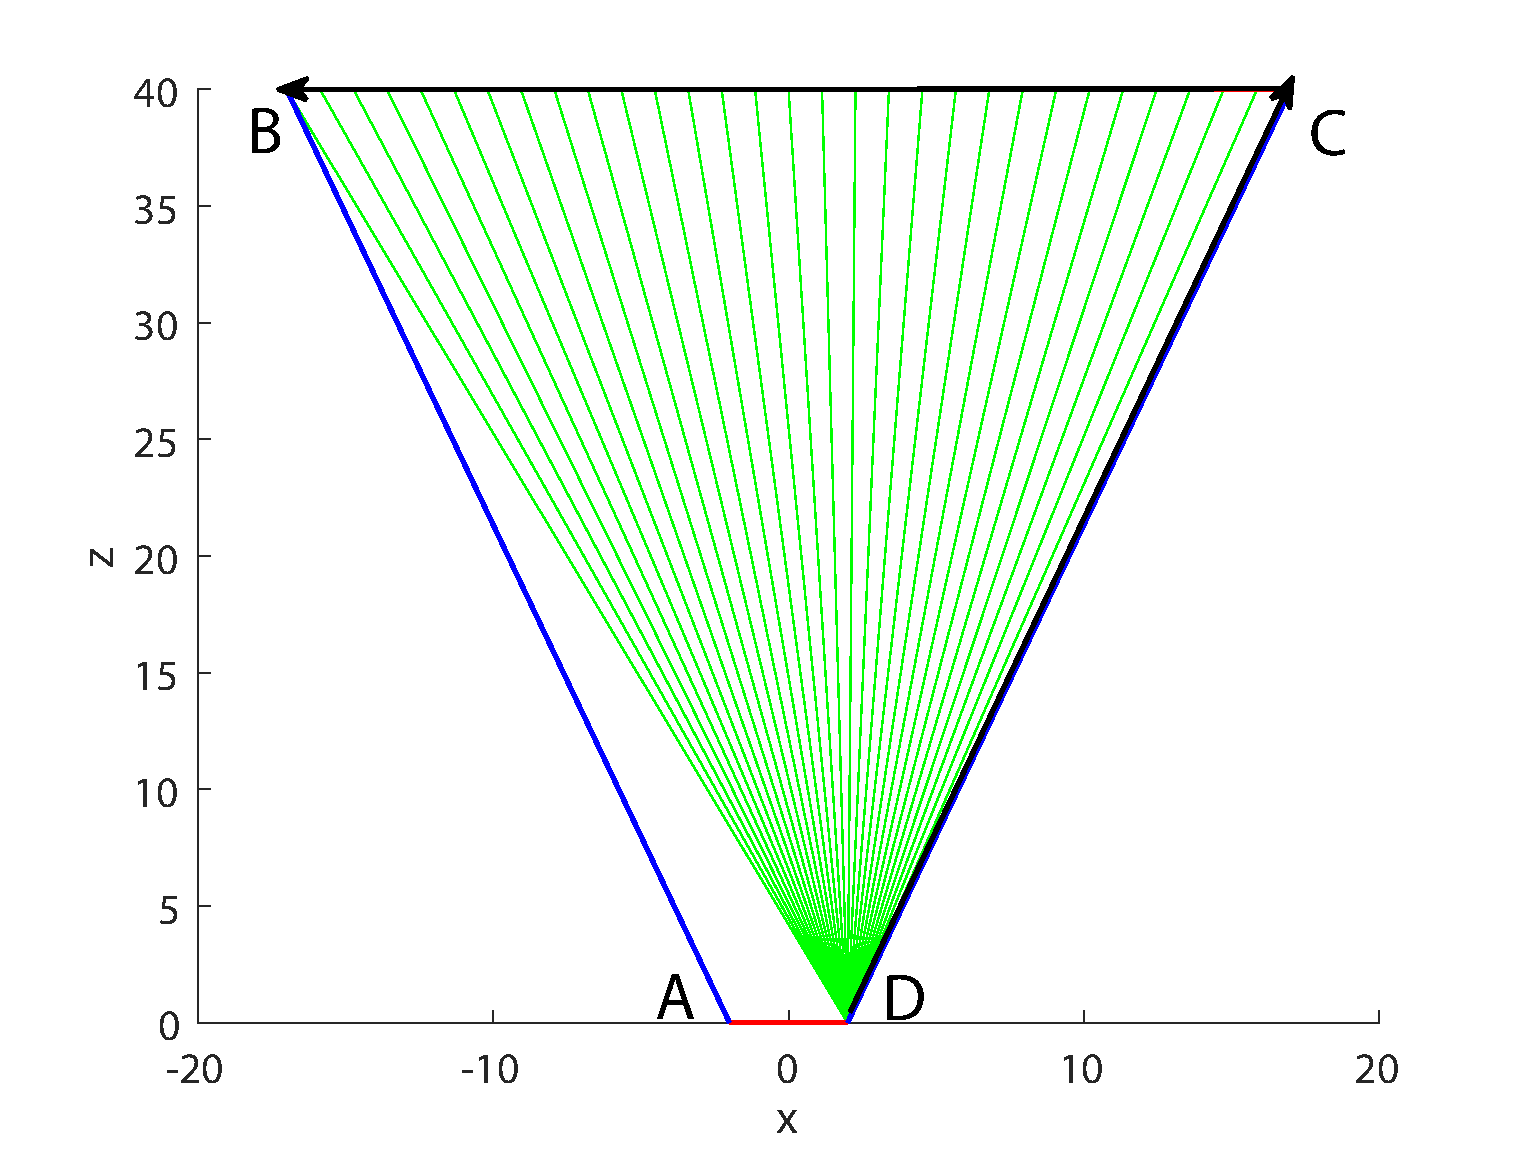
\includegraphics[width = \textwidth]{rays_cup3}
  \caption{Rays that leave the right end point of the source (line $1$) and trace out the target (line $4$).}
  \label{fig:cup3}
\end{subfigure}%
\hfill
\begin{subfigure}{.48\textwidth}
  \centering
  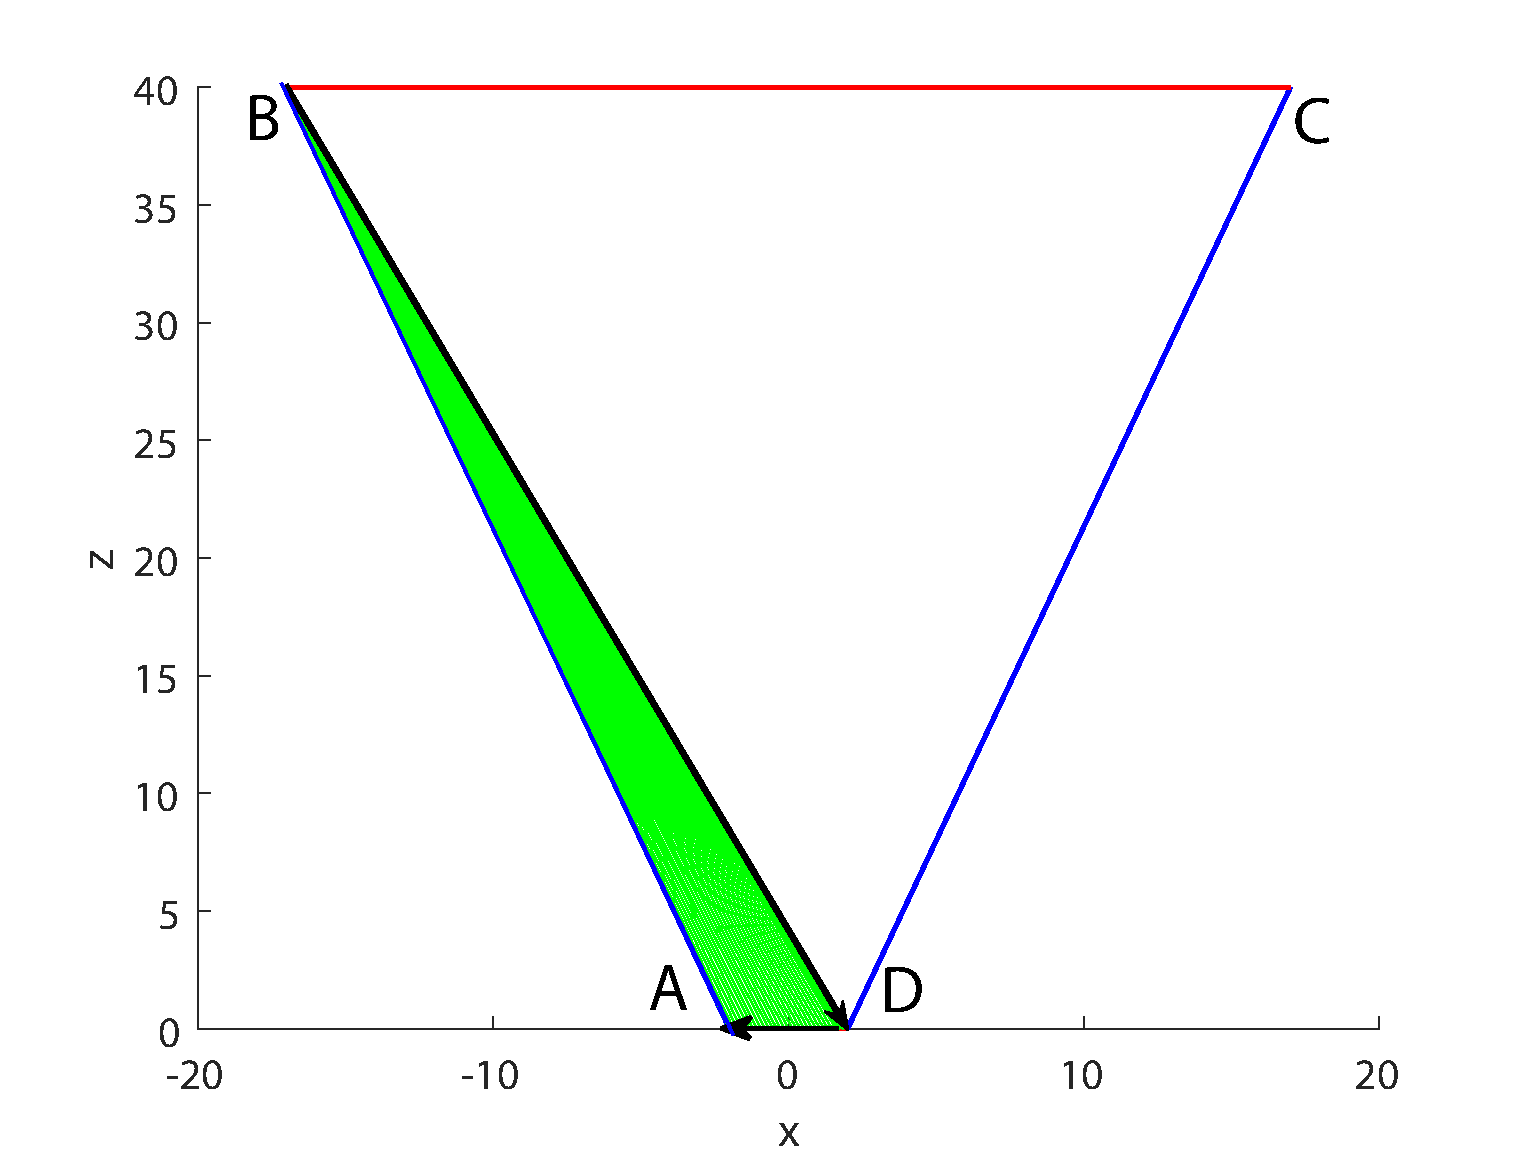
\includegraphics[width=\textwidth]{rays_cup4}
  \caption{Rays that trace out the source (line $1$) and hit the left end point of the target (line $4$).}
  \label{fig:cup4}
\end{subfigure}
\caption{\textbf{Rays located on the boundaries of the regions $\partial$\set{S}{$1$,}{$4$} and $\partial$\set{T}{$4$,}{$1$}}.
$A = (\variabile{x}_{1 \ell}, \variabile{z}_{1, \ell}) =(-2, 0)$ and 
$D = (\variabile{x}_{1, \textrm{r}}, \variabile{z}_{1, \textrm{r}}) = (2, 0)$ 
are the left and right corner points (or end points) of
\point{S} (line $1$).
$B =  (\variabile{x}_{4, \ell}, \variabile{z}_{4, \ell}) = (-17, 40)$ and $C =  (\variabile{x}_{4, \textrm{r}}, \variabile{z}_{4, \textrm{r}}) = (17 , 40)$, are the left and right corner points of \point{T} (line $4$).}
\label{fig:cups}
\end{figure} \\
 The boundaries $\partial$\set{S}{$1$,}{$4$} and $\partial$\set{T}{$4$,}{$1$} are given in Figures \ref{fig:S14} and \ref{fig:T411}, respectively.
$\partial$\setbound{S}{$1$,}{$4$}{1} and $\partial$\setbound{T}{$4$,}{$1$}{1} are obtained tracing out line $4$ from
$\variabile{q}_{\ell} = -\variabile{b}$ to $\variabile{q}_{\textrm{r}} = \variabile{b}$
 by rays leaving $\variabile{q}_{1, \ell}= -\variabile{a}$ with varying $\variabile{p}_1$, these rays are shown in Figure \ref{fig:cup1}, and the boundary segments
 $\partial$\setbound{S}{$1$,}{$4$}{1} and $\partial$\setbound{T}{$4$,}{$1$}{1} are the orange line segments labeled with \const{c}. 
 $\partial$\setbound{S}{$1$,}{$4$}{2} and $\partial$\setbound{T}{$4$,}{$1$}{2} are given tracing out line $1$ from
 $\variabile{q}_{1, \ell}= -\variabile{a}$ to $\variabile{q}_{1, \textrm{r}}= \variabile{a}$
 with varying $\variabile{p}_1$, such that all rays hit $\variabile{q}_{\textrm{r}} = \variabile{b}$, these rays are shown in Figure \ref{fig:cup2}, the boundary segments
 $\partial$\setbound{S}{$1$,}{$4$}{2} and $\partial$\setbound{T}{$4$,}{$1$}{2} are depicted in blue (lines segments labeled with \const{d}).
 Likewise, $\partial$\setbound{S}{$1$,}{$4$}{3} and $\partial$\setbound{T}{$4$,}{$1$}{3} are obtained tracing out line $4$ from
$\variabile{q}_{\textrm{r}}= \variabile{b}$ to $\variabile{q}_{\ell}= -\variabile{b}$ 
 by rays leaving $\variabile{q}_{1, \textrm{r}}=\variabile{x}_{1, \textrm{r}} = \variabile{a}$ with varying $\variabile{p}_{1}$. These rays are shown in Figure \ref{fig:cup3}, 
 $\partial$\setbound{S}{$1$,}{$4$}{3} and $\partial$\setbound{T}{$4$,}{$1$}{3} are the red line segments labeled with \const{e}.
  Finally, $\partial$\setbound{S}{$1$,}{$4$}{4} and $\partial$\setbound{T}{$4$,}{$1$}{4} are given tracing out line $1$ from
$\variabile{q}_{1, \textrm{r}} = \variabile{a}$ to  $\variabile{q}_{1, \ell} = -\variabile{a}$ 
 with varying $\variabile{p}_{1}$, such that all rays hit $\variabile{q}_{\ell} = -\variabile{b}$, these rays are shown in Figure \ref{fig:cup4}, 
 $\partial$\setbound{S}{$1$,}{$4$}{4} and $\partial$\setbound{T}{$4$,}{$1$}{4} are the green lines segments labeled with \const{f}. 
We remind the reader that we use the notation $(\variabile{x}, \variabile{z})$ for the Cartesian coordinates of the optical system, while PS has $(\variabile{q}, \variabile{p})$ coordinates. 
It is worth noting that  $\variabile{q}_{1, \ell}=\variabile{x}_{1, \ell}$,  $\variabile{q}_{1, \textrm{r}}=\variabile{x}_{1, \textrm{r}}$,  
$\variabile{q}_{\ell}=\variabile{x}_{4, \ell}$ and  $\variabile{q}_{\textrm{r}}=\variabile{x}_{4, \textrm{r}}$.\\ \indent
 For the two-faceted cup there is an analytic expression for every line segment $\partial\mbox{\setbound{S}{\lineai,}{\lineaj}{\variabile{\,m}}}$ and
 $\partial\mbox{\setbound{T}{\lineaj,}{\lineai}{\variabile{\,m}}}$ in Equation (\ref{eq:analytic_boundaries}) with $\variabile{m}\in\{1, \cdots, 4\}$.
 For instance, the rays on the boundaries $\partial\mbox{\setbound{S}{\lineai,}{\lineaj}{\,1}}$ and $\partial \mbox{\setbound{T}{\lineaj,}{\lineai}{\,1}}$
  are parameterized in the (\variabile{x}, \variabile{z})-plane by
 \begin{equation}
\label{extremes_rays}
\vect{r}_{\variabile{\lineai}, \variabile{\lineaj}}(\variabile{t})=
\left( \begin{array}{cc}
\variabile{x}_{\variabile{\lineaj}, \ell}-\variabile{x}_{\variabile{\lineai}, \ell}+t(\variabile{x}_{\variabile{\lineaj}, \textrm{r}}-\variabile{x}_{\variabile{\lineaj}, \ell}) \\
\variabile{z}_{\variabile{\lineaj}, \ell}-\variabile{z}_{\variabile{\lineai}, \ell}+t(\variabile{z}_{\variabile{\lineaj}, \textrm{r}}-\variabile{z}_{\variabile{\lineaj},\ell})
\end{array} \right) \qquad \quad 0\leq t\leq 1\,.
\end{equation}
 These rays are located on a vertical line segment in \set{S}{\lineai}{} as only the $\mbox{\variabile{p}}_{\variabile{\lineai}}$-coordinate changes and on a curved line in 
\set{T}{\lineaj}{}
  as both the target position and direction vary. The analytic expressions for $\partial \mbox{\setbound{S}{\lineai,}{\lineaj}{\,1}}$ and $\partial \mbox{\setbound{T}{\lineaj,}{\lineai}{\,1}}$ are
\begin{equation}
\label{S_boundary}
\partial \mbox{\setbound{S}{\lineai,}{\lineaj}{1}}(\variabile{t})= \bigg\{ (\variabile{q}_{\variabile{\lineai}}, \variabile{p}_{\variabile{\lineai}}) = \Big(\variabile{q}_{\variabile{\lineai}, \ell},
|\boldsymbol{\nu}_{\variabile{\lineai}}\times \hat{\vect{r}}_{\variabile{\lineai}, \variabile{\lineaj}}(\variabile{t})|
\Big) \bigg\},
\end{equation}
\begin{equation}
\label{T_boundary}
\partial\mbox{\setbound{T}{\lineaj,}{\lineai}{\,1}}(\variabile{t})=\bigg\{(\variabile{q}_{\variabile{\lineaj}}, \variabile{p}_{\variabile{\lineaj}}) =
\Big(\variabile{q}_{\variabile{\lineaj}, \ell}-\variabile{q}_{\variabile{\lineai}, \ell}+t(\variabile{q}_{\variabile{\lineaj}, \textrm{r}}-\variabile{q}_{\variabile{\lineaj},\ell}),
|\boldsymbol{\nu}_{\variabile{\lineaj}}\times \hat{\vect{r}}_{\variabile{\lineai}, \variabile{\lineaj}}(\variabile{t})|\Big) \bigg\}\,,
\end{equation}
where we have indicated with $\hat{\vect{r}}_{\variabile{\lineai}, \variabile{\lineaj}}(\variabile{t})$ the normalization of the ray in ($\ref{extremes_rays}$) and
 $ \boldsymbol{\nu}_\variabile{\lineai}$ and $\boldsymbol{\nu}_\variabile{\lineaj}$ are the normalized inward normals to lines $\variabile{\lineai}$ and $\variabile{\lineaj}$, respectively.
 Note that  $\sin{\tau_\variabile{\lineai}} = |\nu_{\variabile{\lineai}}\times \hat{\vect{r}}_{\variabile{\lineai}, \variabile{\lineaj}}(\variabile{t})|$ and $\sin{\tau_\variabile{\lineaj}} = |\nu_{\variabile{\lineaj}}\times \hat{\vect{r}}_{\variabile{\lineai}, \variabile{\lineaj}}(\variabile{t})|$.
 \begin{figure}
 \begin{minipage}[]{.48\textwidth}
   \centering
   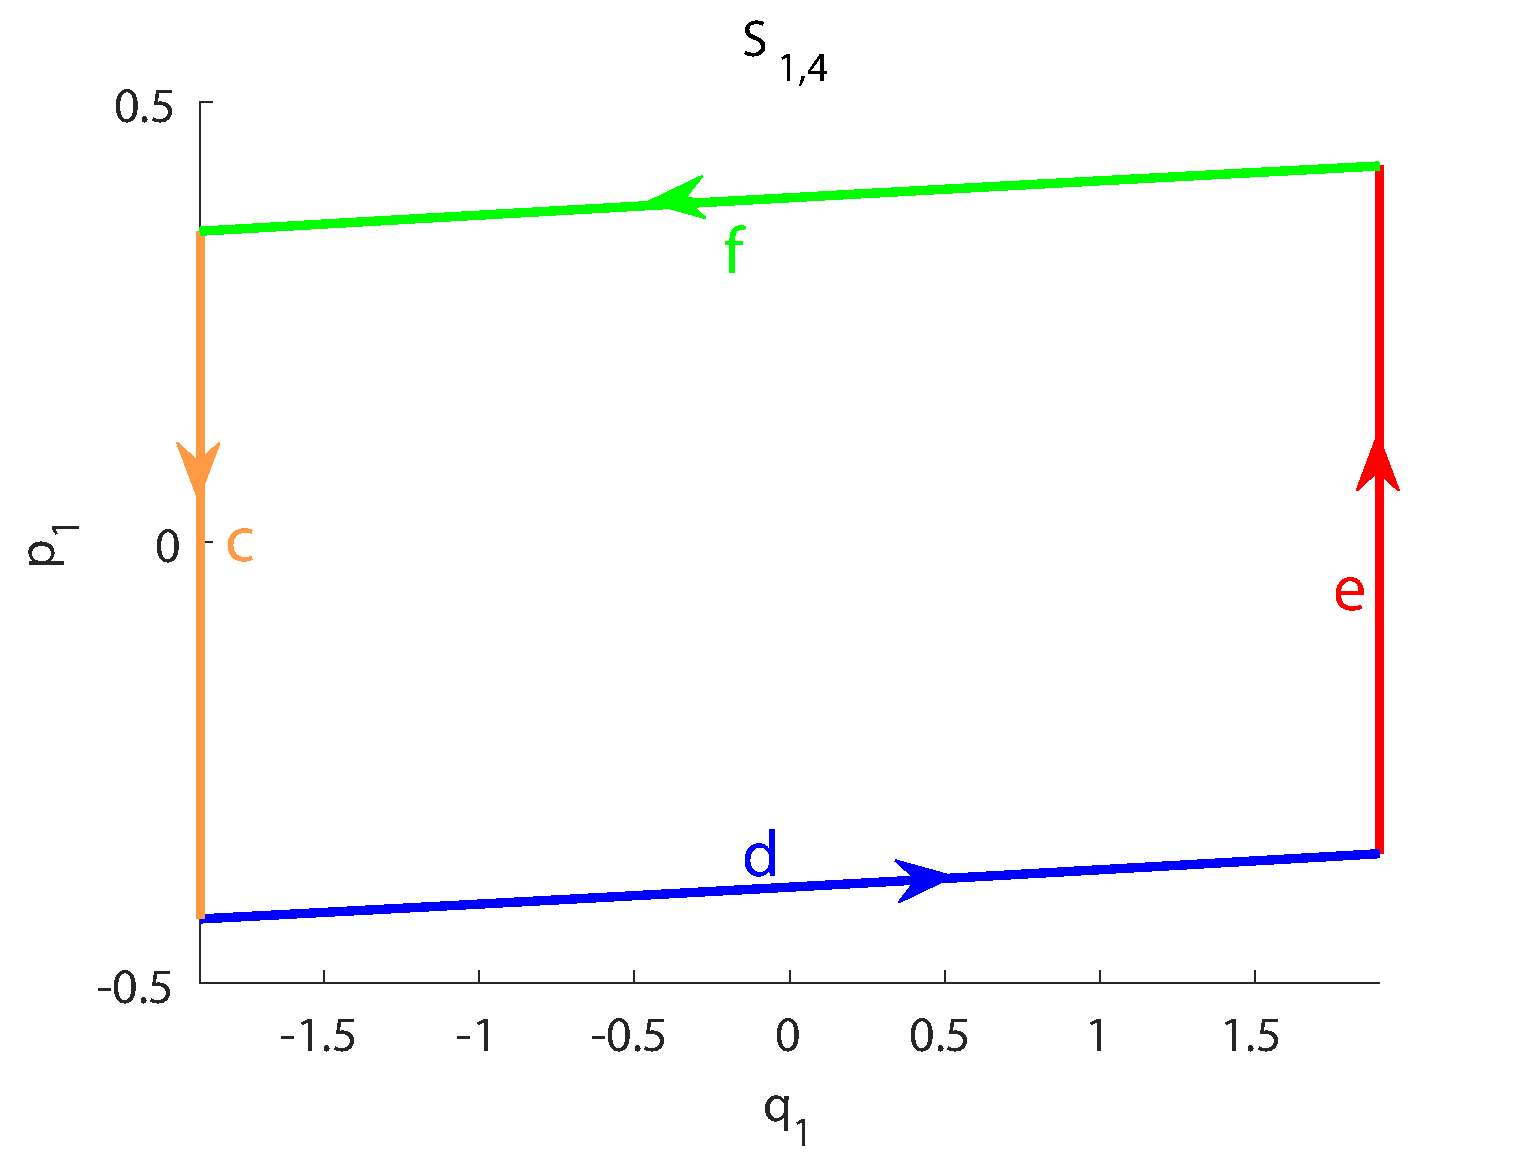
\includegraphics[width=\textwidth]{S141}
   \caption{\textbf{Source PS of line $1$.}
   Boundary of the region \set{S}{$1$,}{$4$}.}
   \label{fig:S14}
 \end{minipage}\hfill
  \begin{minipage}[]{0.48\textwidth}
  \centering
   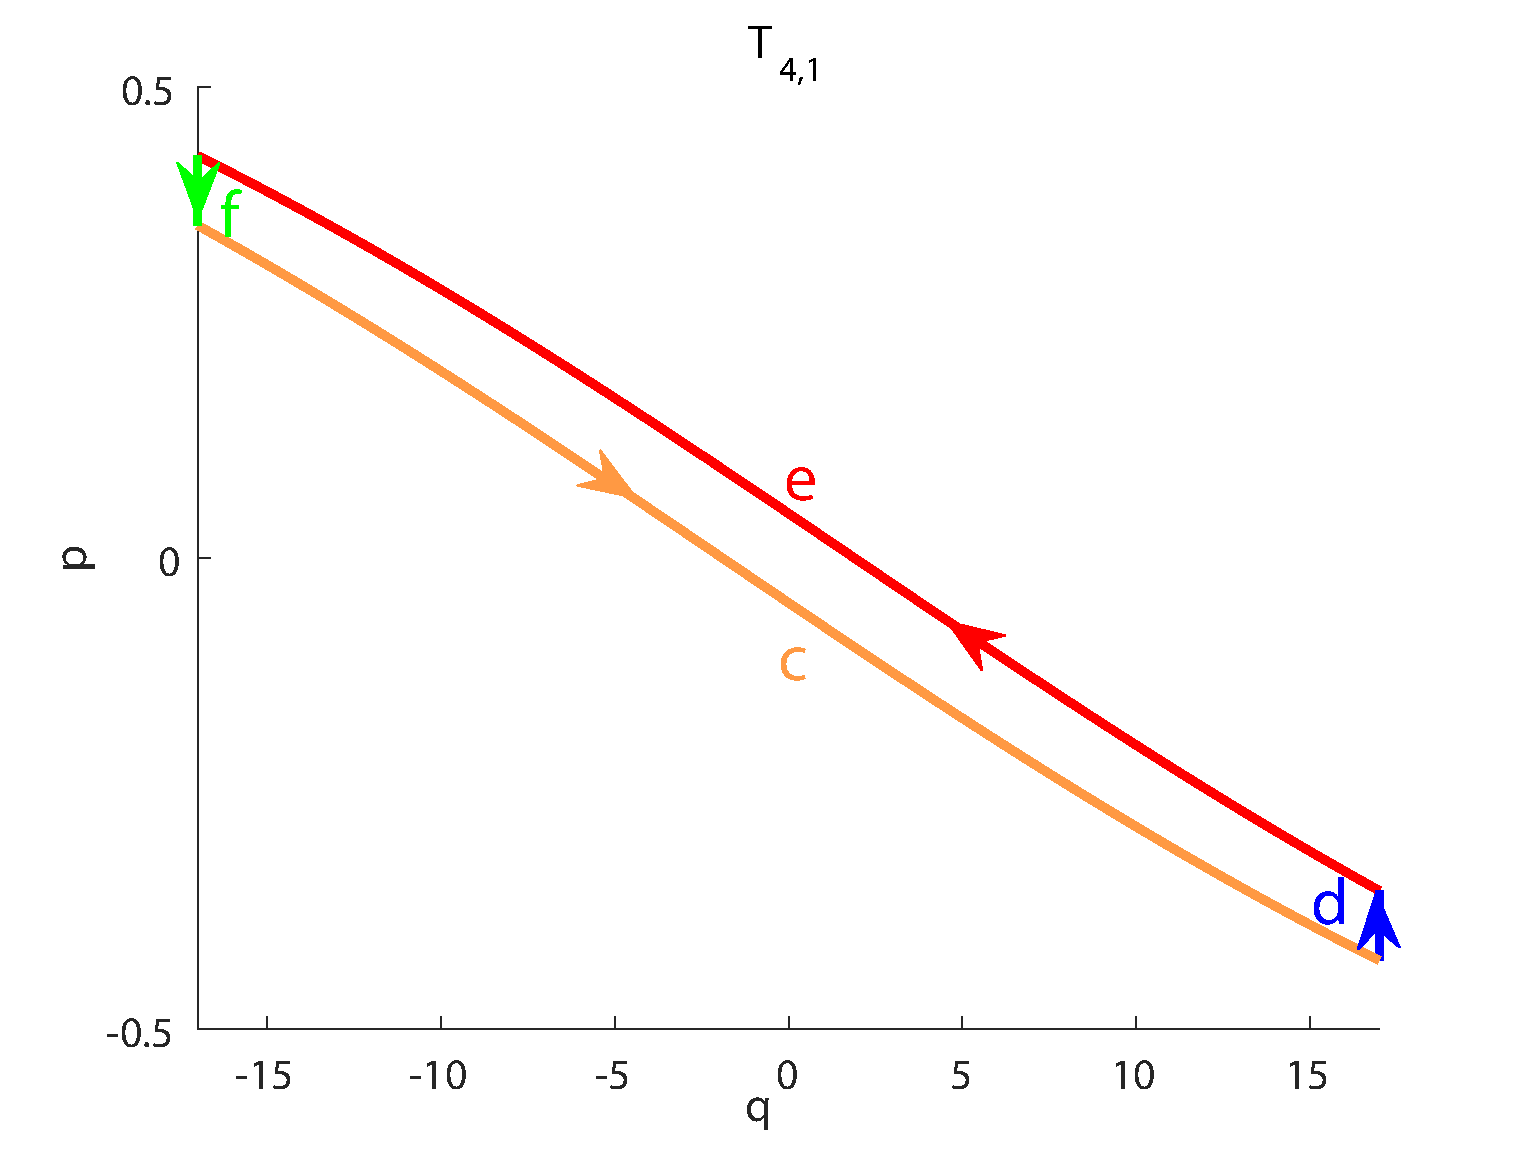
\includegraphics[width=\textwidth]{T411}
   \caption{\textbf{Target PS of line $4$.}
    Boundary of the region \set{T}{$4$,}{$1$}.}
    \label{fig:T411}
 \end{minipage}
 \end{figure}
 Likewise, the boundaries $\partial$\setbound{S}{\lineai,}{\lineak}{\variabile{\,m}} and
 $\partial$\setbound{T}{\lineak,}{\lineai}{\variabile{\,m}} are calculated for every $\variabile{m}\in\{2,3,4\}$. Finally, $\partial$\set{S}{\lineai,}{\lineak} and $\partial$\set{T}{\lineak,}{\lineai} are determined using (\ref{eq:analytic_boundaries}). \\
 \begin{figure}
 \begin{minipage}[]{.43\textwidth}
   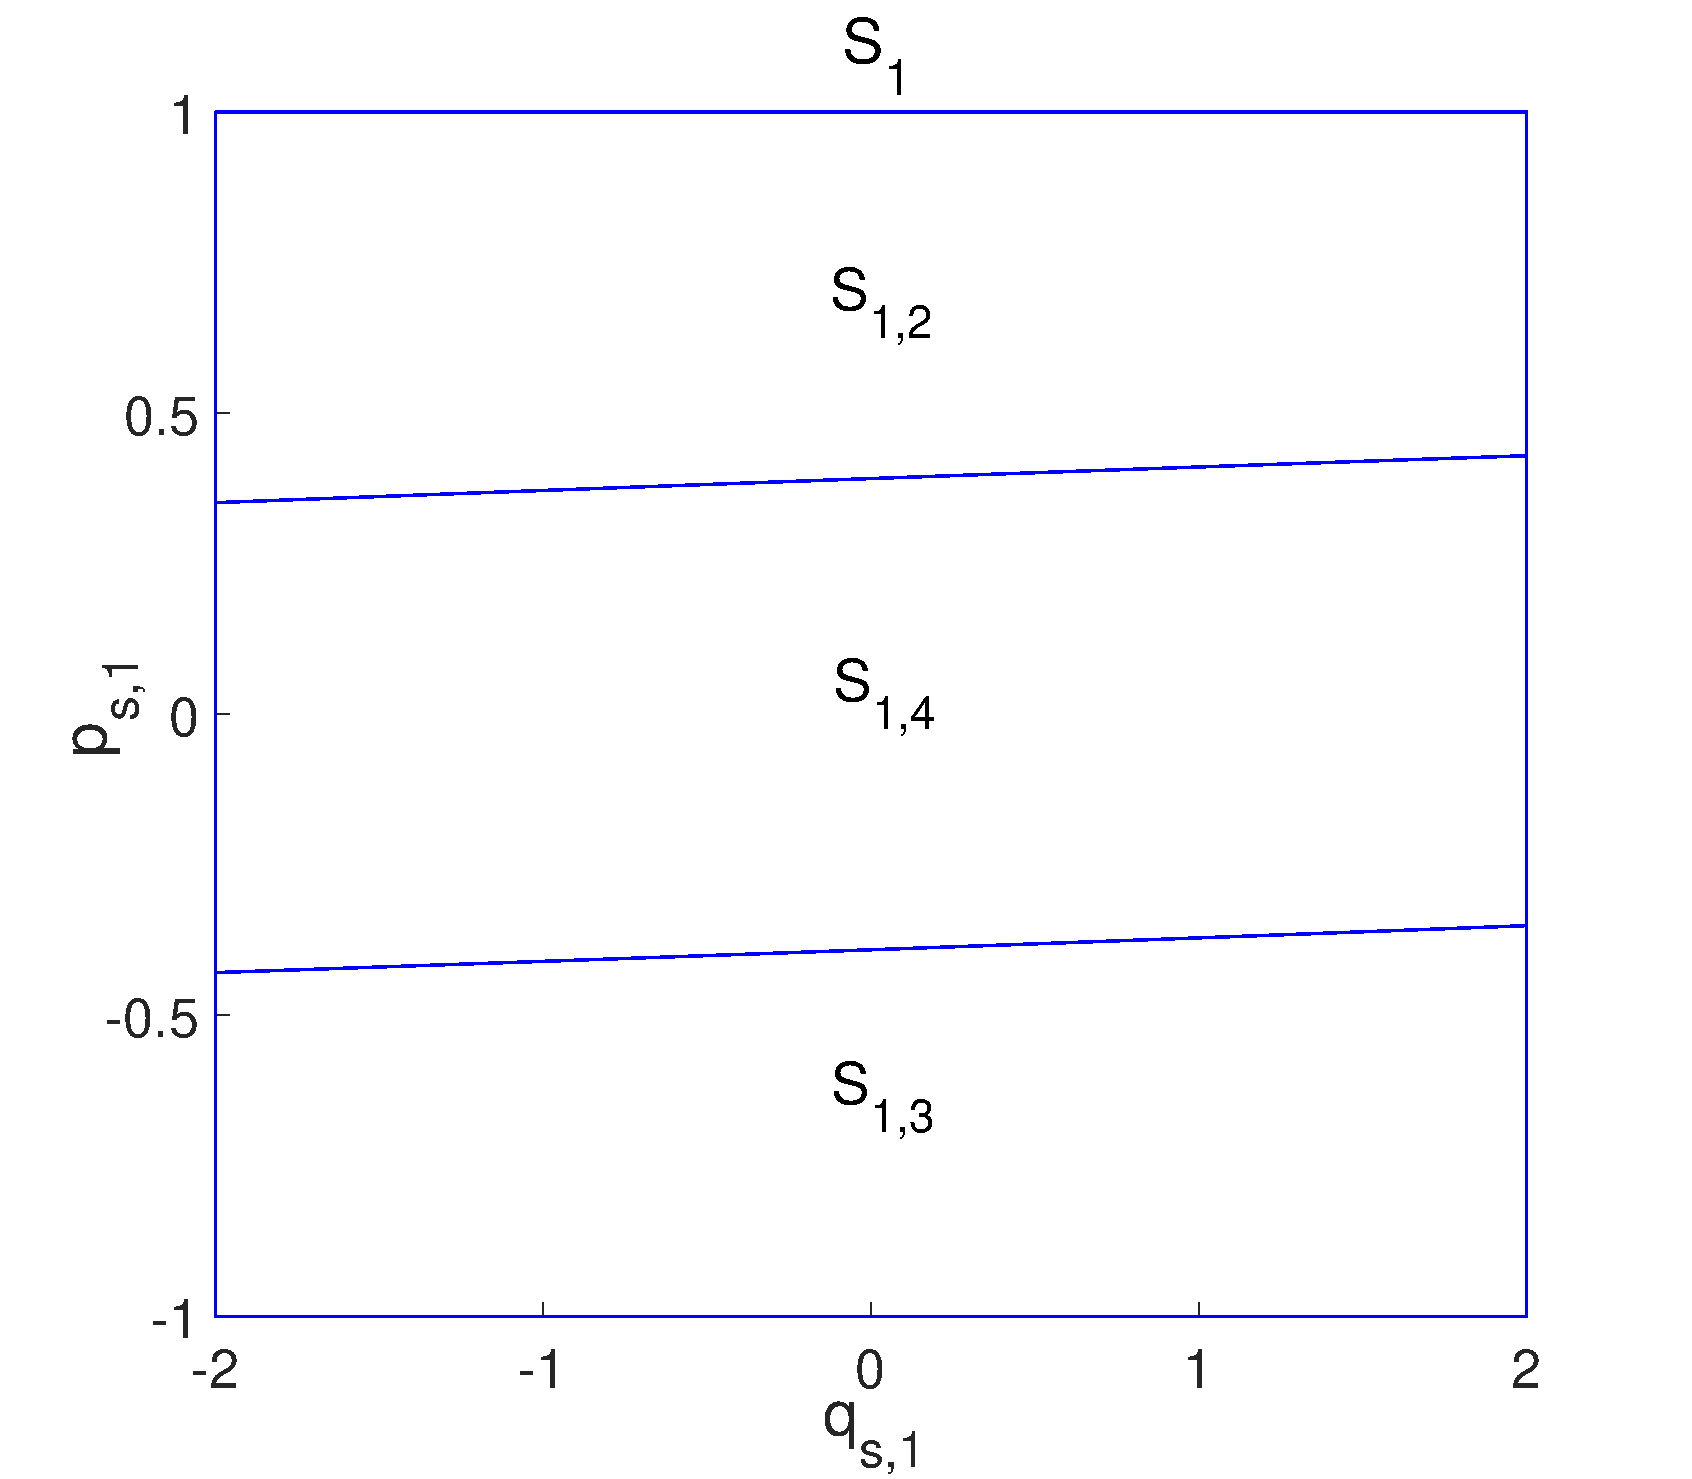
\includegraphics[width=\textwidth]{S1}
\caption{\footnotesize{\textbf{Source PS of line $\boldsymbol{1}$.} It is partitioned into regions $(\mbox{\set{S}{$1$,}{\lineaj}})_{\variabile{\lineaj} = 2,3,4}$
   formed by rays that leave line $1$ and hit line $\textit{\lineaj}$.}}
   \label{fig:S1}
 \end{minipage}
  \begin{minipage}[]{.45\textwidth}
  \centering
   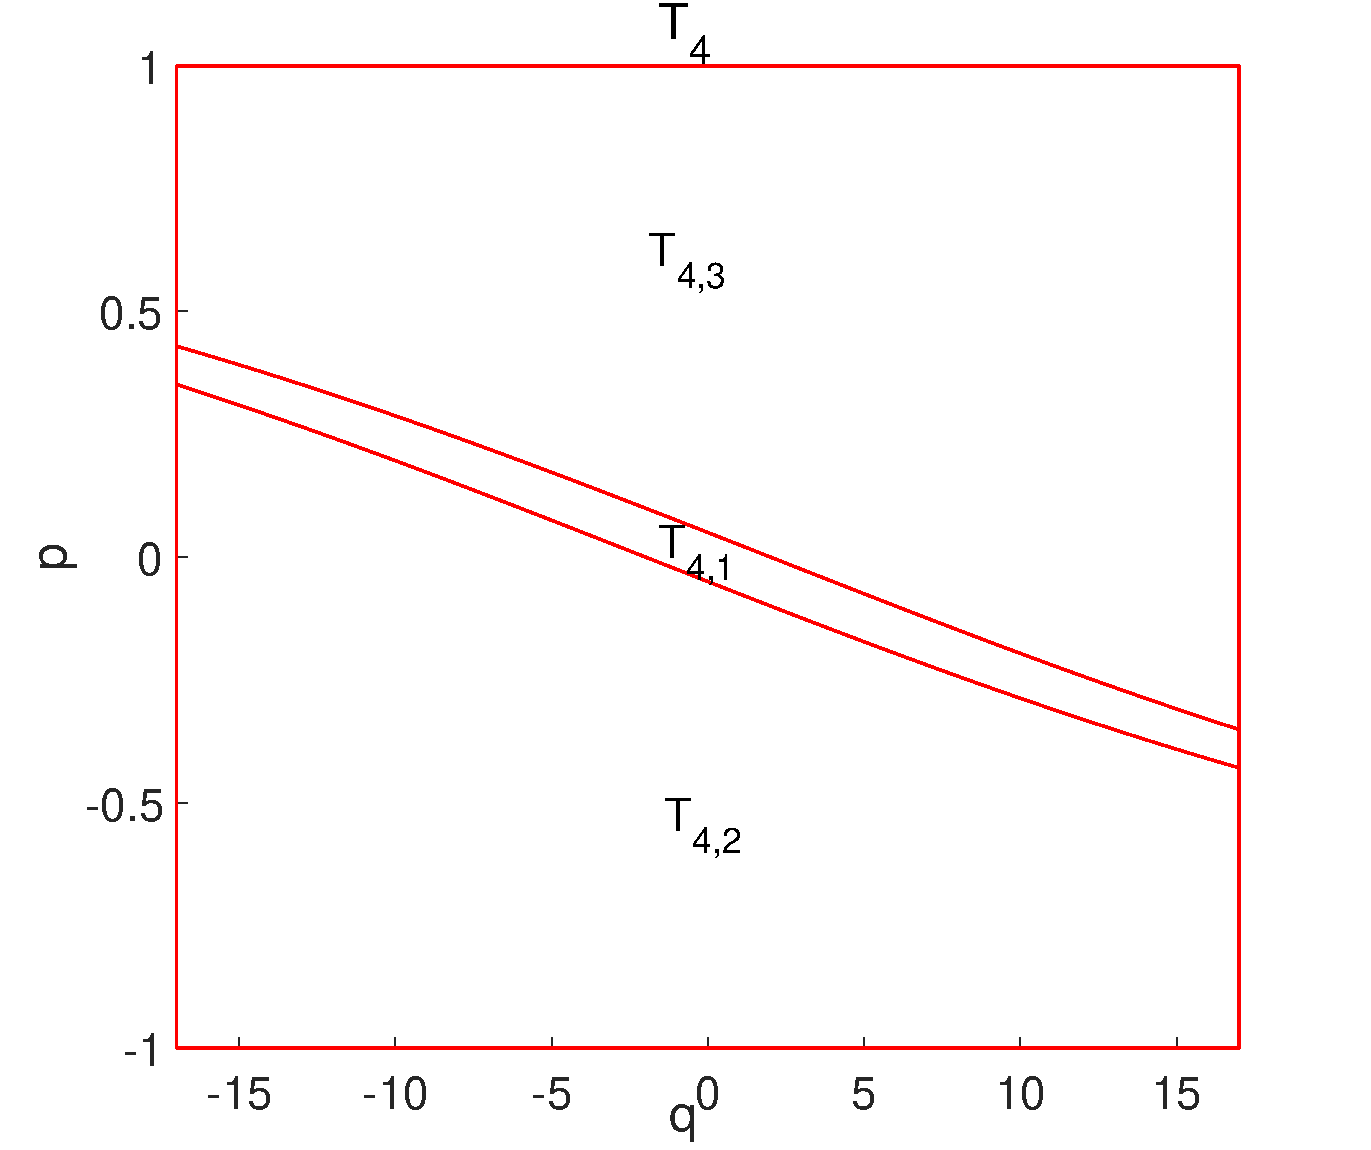
\includegraphics[width=\textwidth]{T4b}
   \caption{\footnotesize{\textbf{Target PS of line $\boldsymbol{4}$.} It is partitioned into regions $(\mbox{\set{T}{$4$,}{\lineak}})_{\variabile{\lineak} = 1,2,3}$
   formed by rays that leave line $\textit{\lineak}$ and hit line $4$.}}
   \label{fig:T4b}
 \end{minipage}
\begin{minipage}[]{.43\textwidth}
\centering
   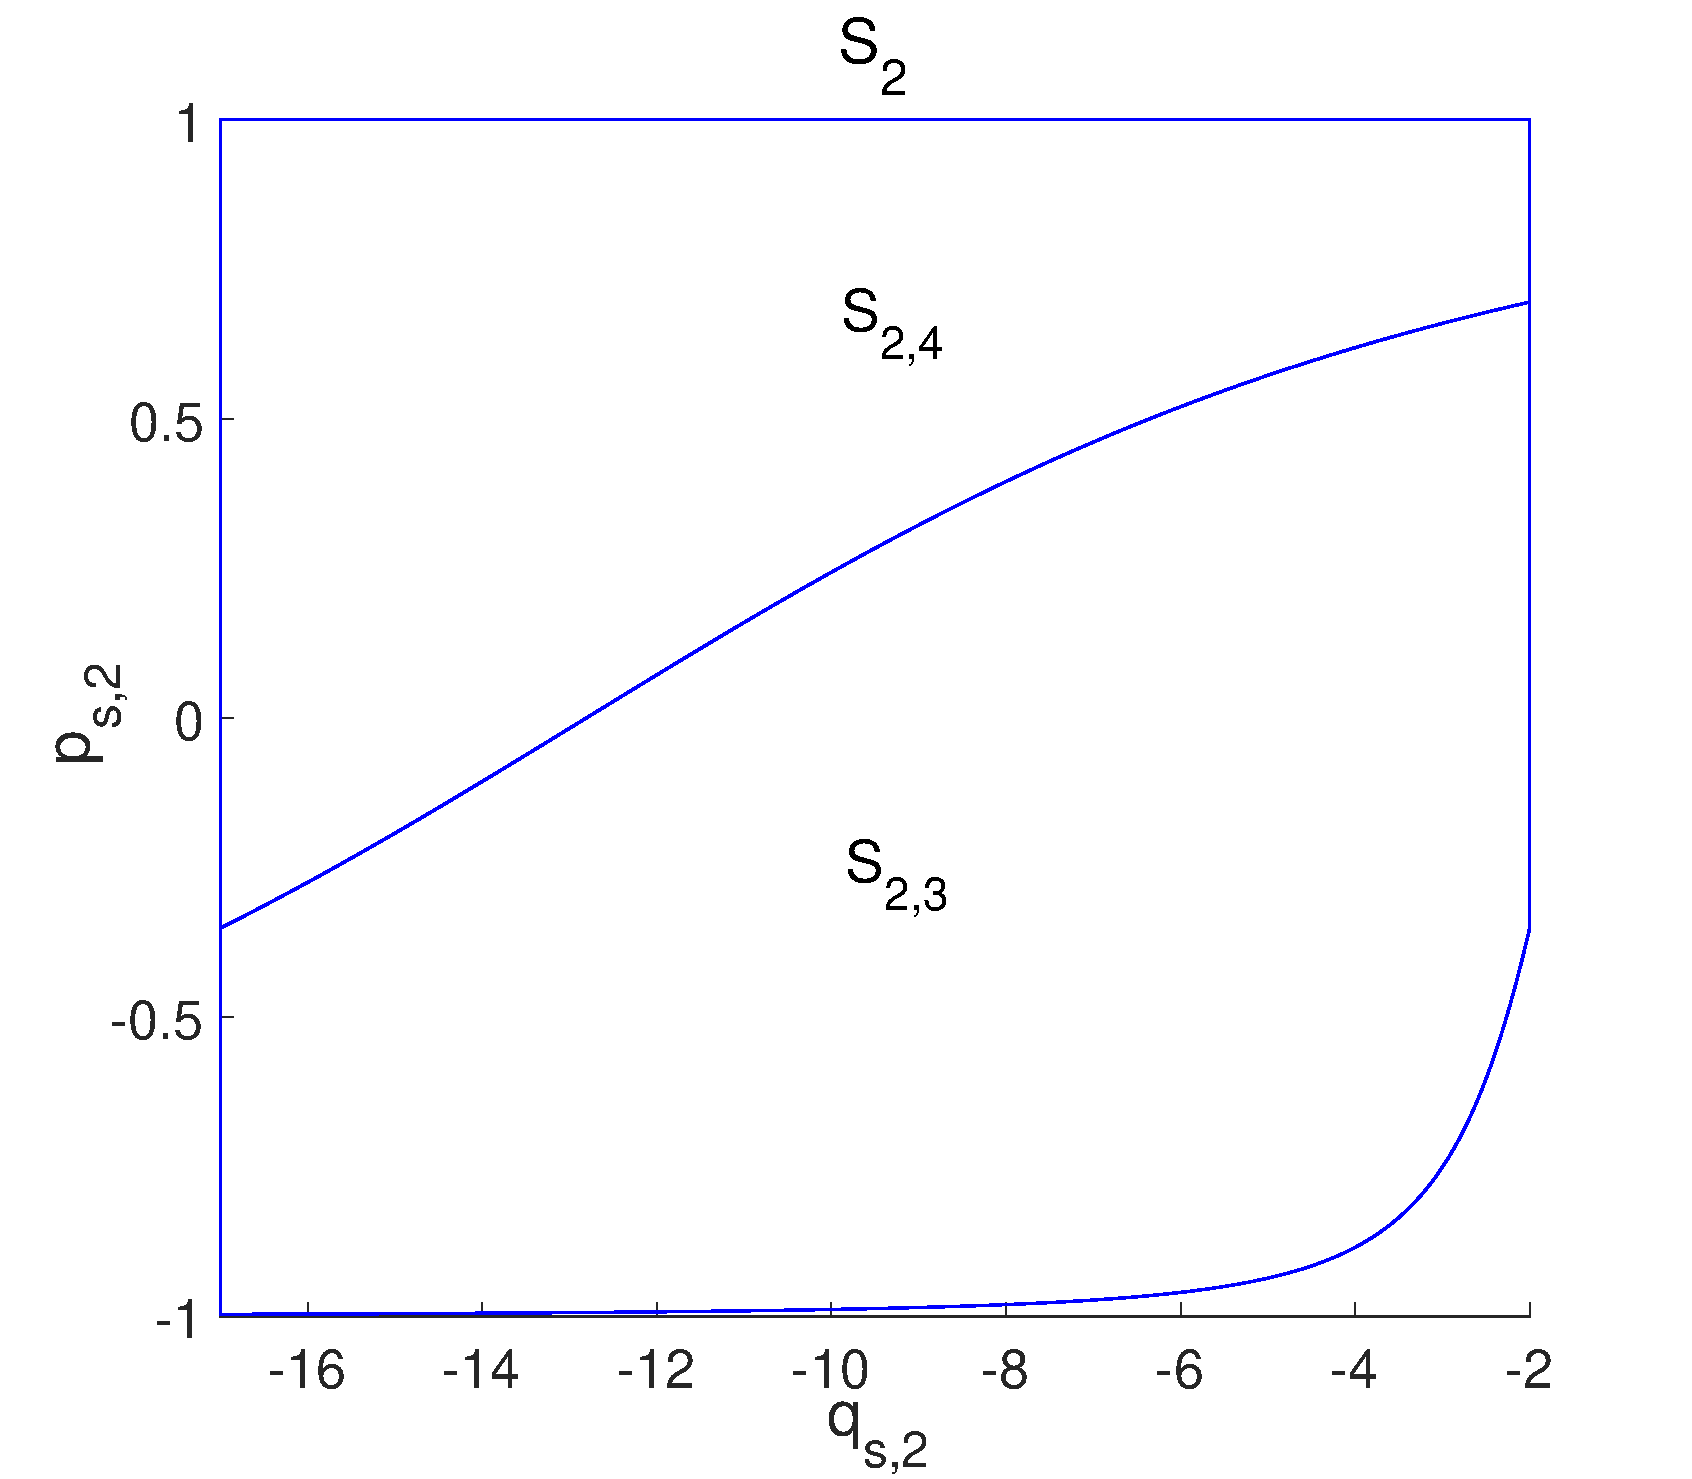
\includegraphics[width=\textwidth]{S2}
\caption{\footnotesize{\textbf{Source PS of line $\boldsymbol{2}$.} It is partitioned into regions $(\mbox{\set{S}{$2$,}{\lineaj}})_{\variabile{\lineaj} = 3,4}$
  formed by rays that leave line $2$ and hit line $\variabile{\lineaj}$.}} 
 \end{minipage}
 \begin{minipage}[]{.43\textwidth}
 \centering
   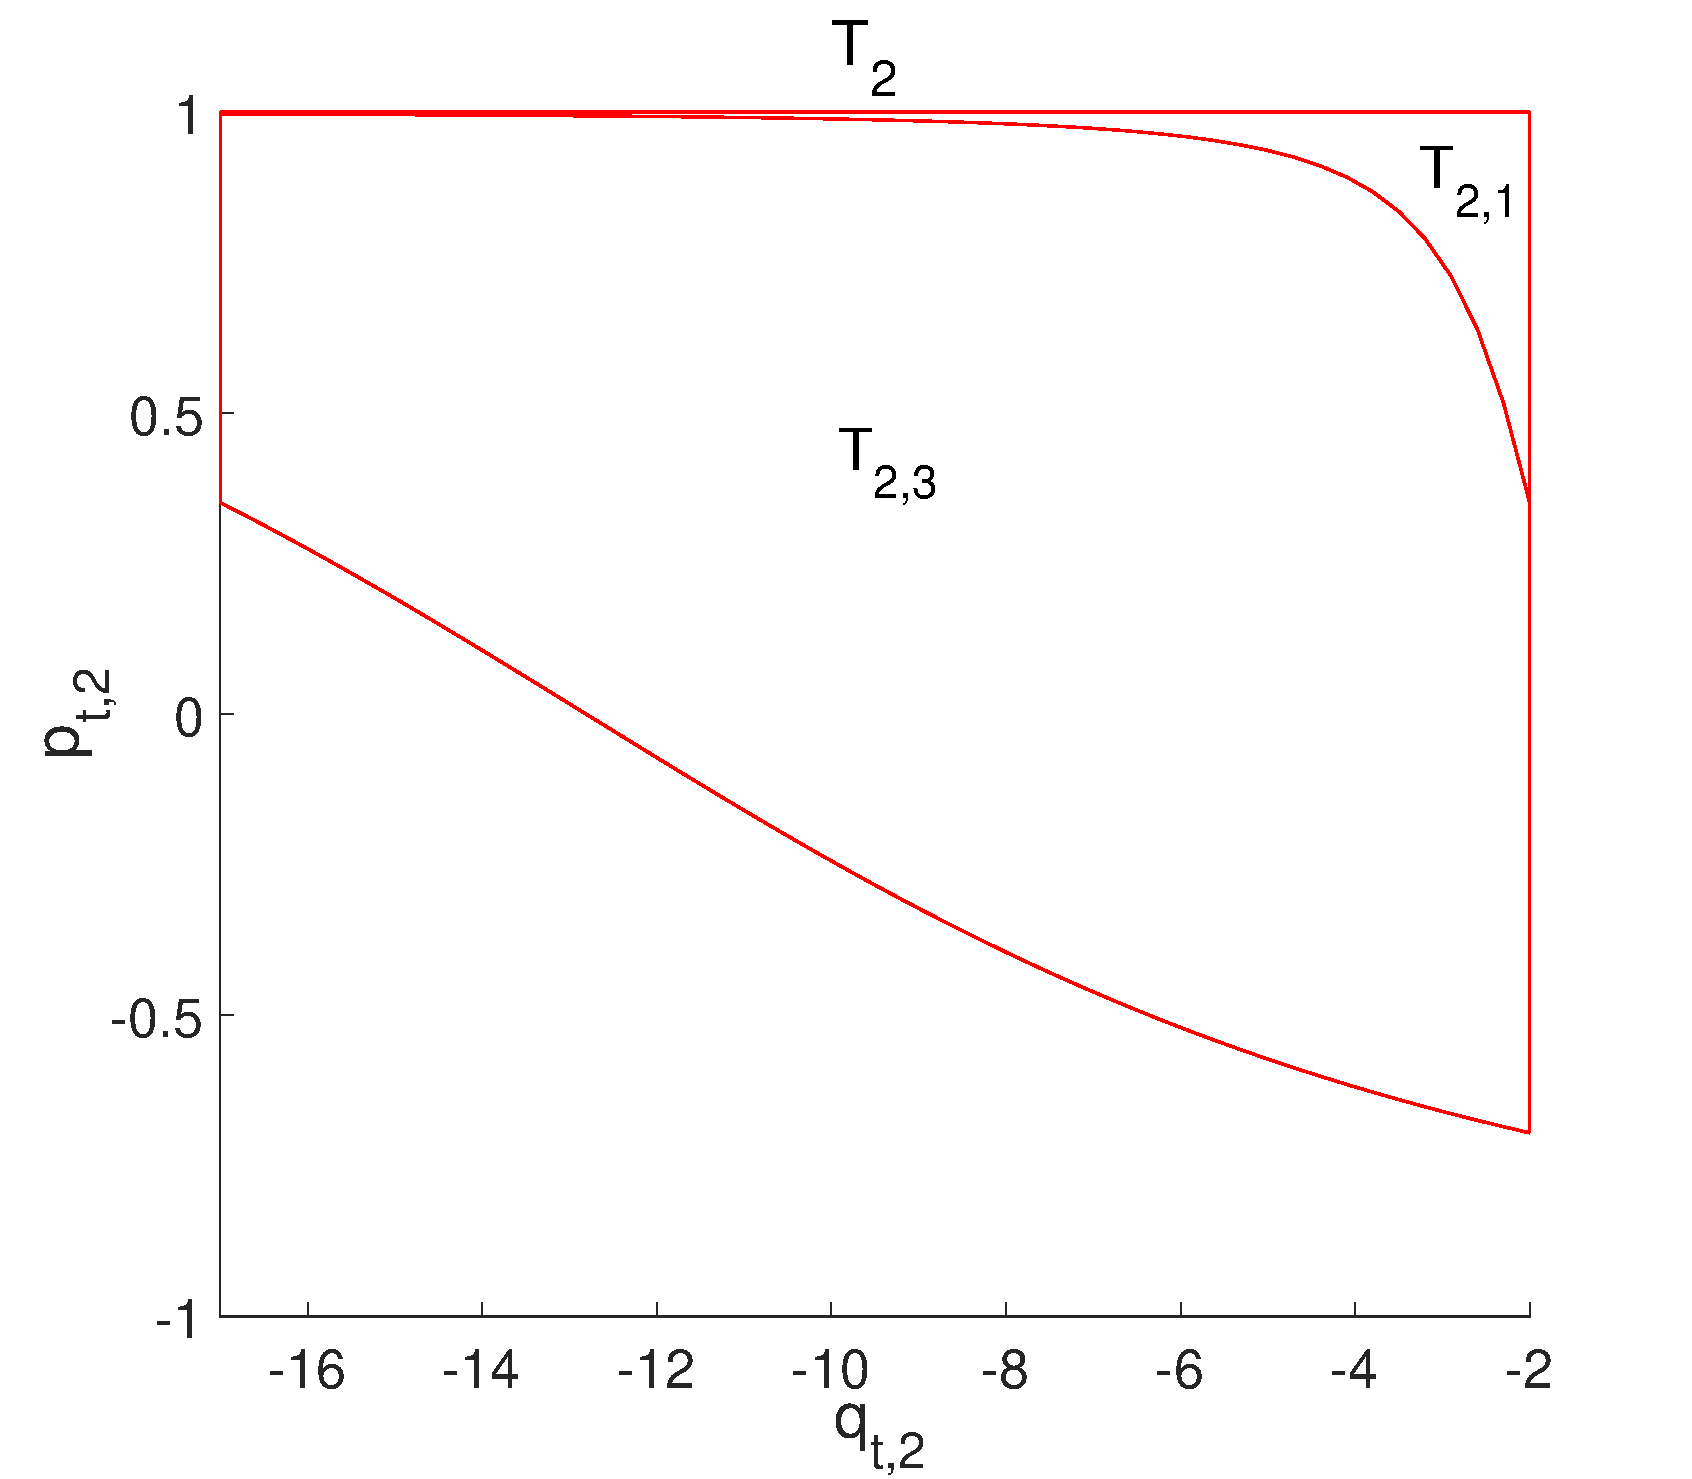
\includegraphics[width=\textwidth]{T2b}
\caption{\footnotesize{\textbf{Target PS of line $\boldsymbol{2}$.} It is partitioned into regions $(\mbox{\set{T}{$2$,}{\lineak}})_{\variabile{\lineak} = 1,3}$
formed by rays that leave line $\variabile{\lineak}$ and hit line $2$. }} 
 \end{minipage}
 \begin{minipage}[]{.43\textwidth}
 \centering
   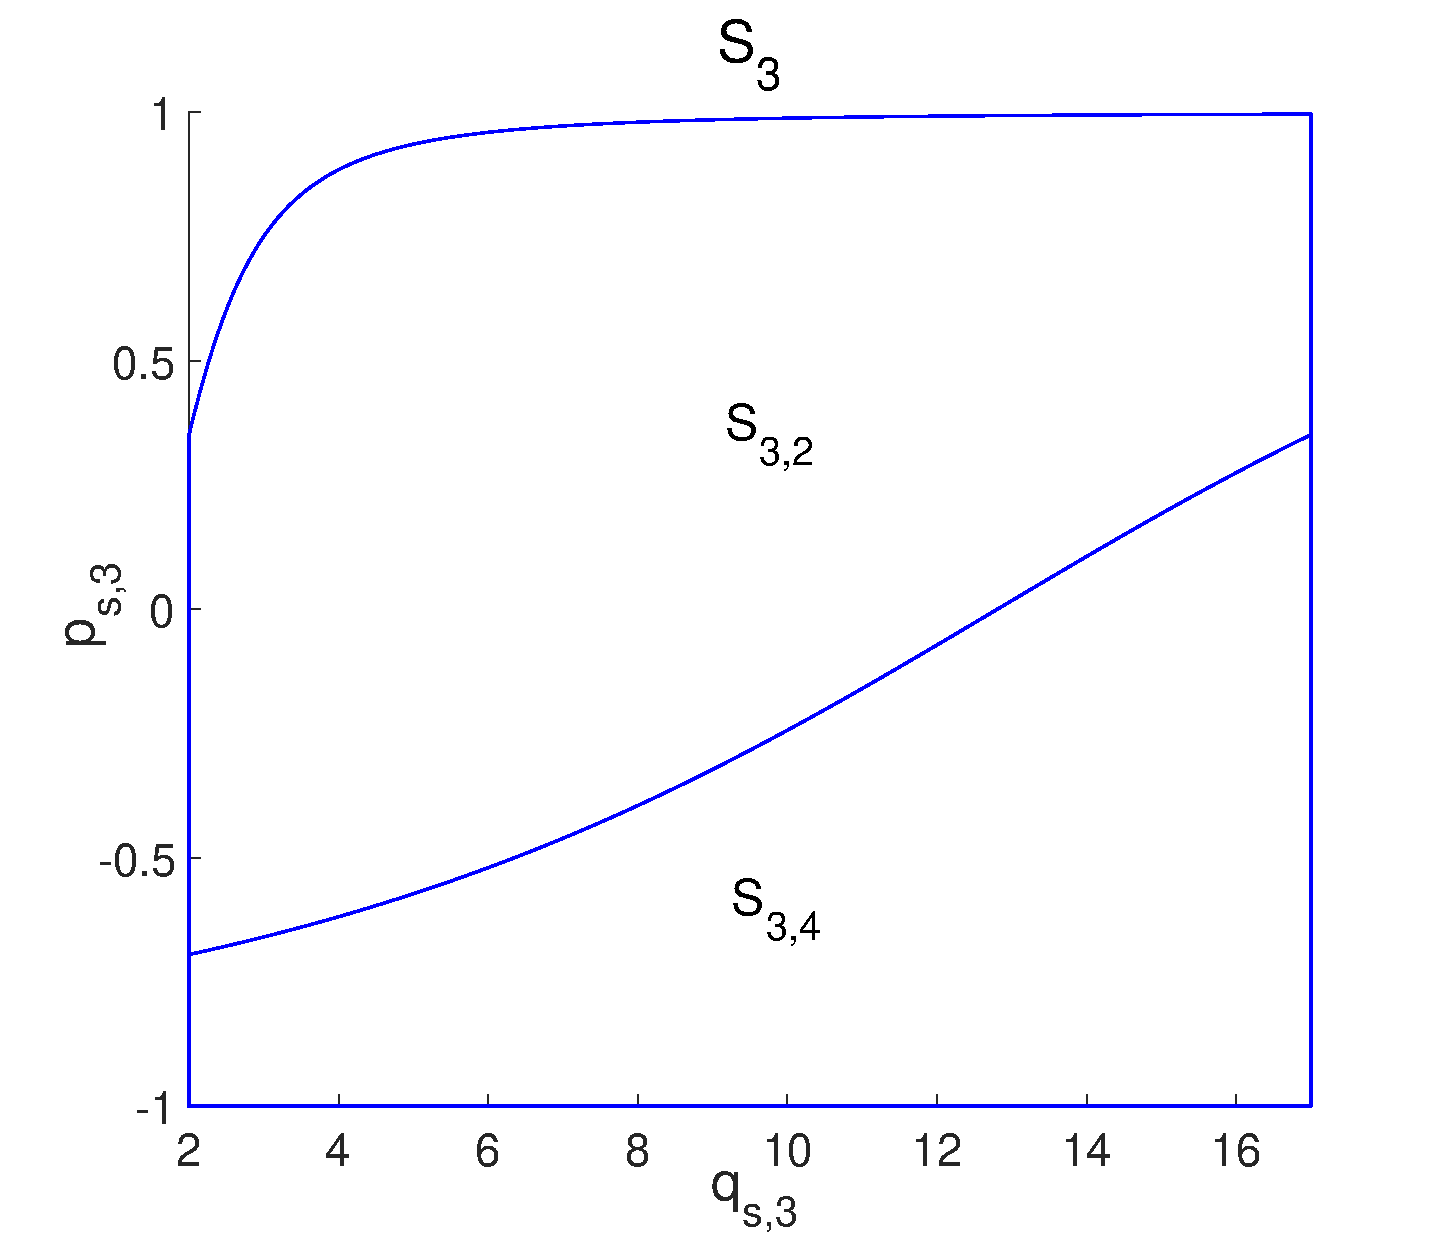
\includegraphics[width=\textwidth]{S3}
   \caption{\footnotesize{\textbf{Source PS of line $\boldsymbol{3}$.} It is partitioned into regions
   $(\mbox{\set{S}{$3$,}{\lineaj}})_{\variabile{\lineaj} = 2,4}$ formed by rays that leave line $3$ and hit line $\variabile{\lineaj}$. }} 
 \end{minipage}
 \hspace{1.7cm}
 \begin{minipage}[]{.43\textwidth}
 \centering
   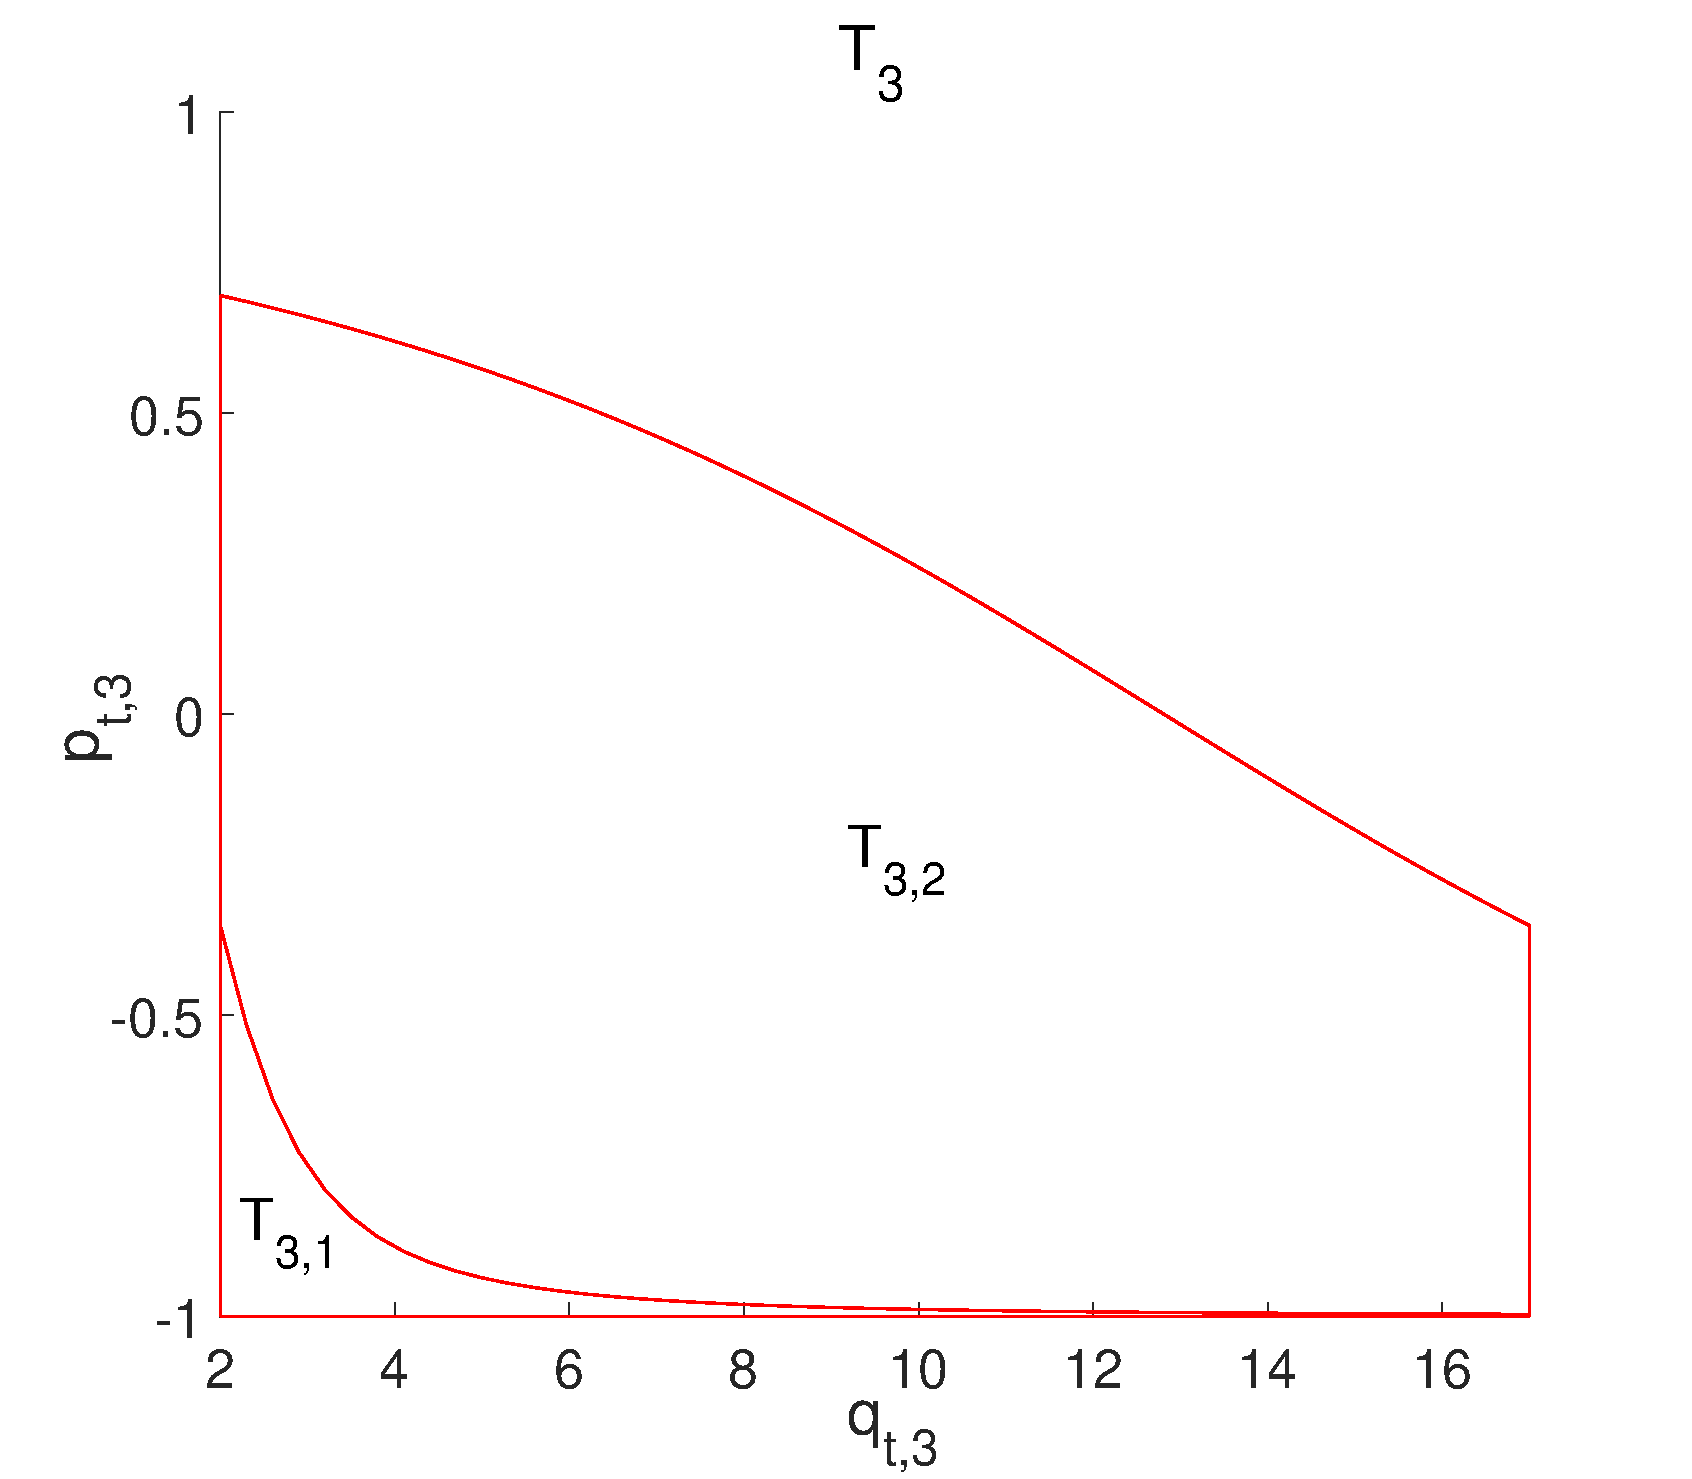
\includegraphics[width=\textwidth]{T3_b}
  \caption{\footnotesize{\textbf{Target PS of line $\boldsymbol{3}$.} It is partitioned into regions $(\mbox{\set{T}{$3$,}{\lineak}})_{\variabile{\lineak} = 1,2}$
   formed by rays that leave line $\variabile{\lineak}$ and hit line $3$.}} 
\label{fig:T3}
 \end{minipage}
\end{figure}
\indent In Figures $\ref{fig:S1}-\ref{fig:T3}$,  $(\partial \mbox{\set{S}{\lineai,}{\lineaj}})_{\variabile{\lineai}\neq\variabile{\lineaj}=2, 3, 4}$ and $(\partial \mbox{\set{T}{\lineai,}{\lineak}})_{\variabile{\lineai}\neq\variabile{\lineak}=1, 2, 3}$ are depicted in blue and red, respectively. The source and target PS of lines $2$ and $3$ have some empty regions. 
These parts correspond to the regions formed by the rays that either go back to the source or are emitted from the target. These regions are not taken into account, see Equation (\ref{SPS}). We observe that, because of the symmetry of the optical system, \set{S}{$3$}{} is the mirror image of \set{S}{$2$}{} after reflection in the central point 
$(\variabile{q}, \variabile{p}) = (-9.5, 0)$ followed by a translation $(\variabile{q}, \variabile{p})\rightarrow(\variabile{q}+19, \variabile{p})$. Likewise \set{T}{$3$}{} is the mirror image of \set{S}{$2$}{} after the same reflection and translation.
%In the next section, we show how the phase spaces are related to each other and we define the target photometric variables on \set{T}{$4$}{}.
\subsection{Computation of the target photometric variables}
In this section we explain how to compute the target photometric variables in PS.
The intensity $I$ along a given direction $\variabile{p}\in [-1,1]$ in target phase space \set{T}{$4$}{} depends on the luminance $L(\variabile{q}, \variabile{p})$ defined as in Equation (\ref{eq:PSintensity}). For the two-faceted cup, it becomes:
\begin{equation}\label{I(eta)}
I_{\textrm{PS}}(\variabile{p}) = \int_{-\variabile{b}}^{\variabile{b}} L(\variabile{q},\variabile{p}) \textrm{d}\variabile{q}\,.
\end{equation}
The parts of \set{T}{$4$}{} that are illuminated by the source \point{S} correspond to parts with positive luminance, for the other parts the luminance might be $0$.
Assuming positive luminance on \point{S}, the following relations hold:
\begin{equation}\label{LT4}
\begin{aligned}
L(\variabile{q}, \variabile{p})&>0 \qquad \quad \forall (\variabile{q}, \variabile{p})\in \mbox{\set{T}{$4$,}{$1$}},\\
L(\variabile{q}, \variabile{p})&\geq 0 \qquad\quad \forall(\variabile{q}, \variabile{p}) \in (\mbox{\set{T}{$4$,}{\lineai}})_{\lineai=2,3}.
\end{aligned}
\end{equation}
Once a ray leaves the source \point{S} it can hit the reflectors several times before hitting the target \point{T}. To relate \point{S} and \point{T}, a map $\mapnumb{M}_{1,4}$: \set{S}{$1$}{}$\rightarrow$ \set{T}{$4$}{} is introduced such that $\mapnumb{M}_{1,4}(\pos{s,}{$1$},\dir{s,}{$1$})=(\variabile{q},\variabile{p})$. As  not all parts of \set{T}{$4$}{} are illuminated by the source \point{S}, the map
$\mapnumb{M}_{1,4}$ is not surjective.
Therefore, we need to determine the subsets of \set{T}{$4$}{} illuminated by \point{S} corresponding to the regions where the luminance is positive.
To this purpose, we consider two different kinds of maps.
The first map relates the coordinates of the source and the target PS of two \textit{different} lines, we call it the \textit{propagation map}.
The second map relates the coordinates of the target and the source PS of the \textit{same} line, we call it the \textit{reflection map}.
In particular, given two lines $\lineai$ and $\lineaj$ with $\lineai\neq\lineaj$, the propagation map $\mapnumb{P}_{\lineai,\lineaj}: \mbox{\set{S}{\lineai,}{\lineaj}}\rightarrow$\set{T}{\lineaj,}{\lineai} relates \set{S}{\lineai,}{\lineaj} with \set{T}{\lineaj,}{\lineai} and, it is defined as follows:
 \begin{equation}\label{Pij}
\mapnumb{P}_{\lineai,\lineaj}(\pos{s,}{\lineai},\dir{s,}{\lineai})=(\pos{t,}{\lineaj},\dir{t,}{\lineaj}),
\end{equation}
where $\pos{t,}{\lineaj}$ is given by the \variabile{x}-coordinate of the intersection point between the ray and line $\lineaj$,
and $\dir{t,}{\lineaj}$ is computed considering the direction of the incident ray with respect to the normal of line $\lineaj$. 
For one single line $\lineaj$, the reflection map $\mapnumb{R}_{\lineaj,\lineak,h}$:~\set{T}{\lineaj,}{\lineak} $\rightarrow$\set{S}{\lineaj,}{h}  relates the regions \set{T}{\lineaj,}{\lineak}$\subset$\set{T}{\lineaj}{} and
\set{S}{\lineaj,}{h}$\subset$\set{S}{\lineaj}. To simplify the notation, from now on we omit the dependence of $\mapnumb{R}_{\lineaj,\lineak,h}$ from $\lineak$ and \variabile{h}, i.e., $\mapnumb{R}_{\lineaj,\lineak,h} = \mapnumb{R}_{\lineaj}$. The reflection map is defined as:
\begin{equation}\label{Rj}
\mapnumb{R}_{\lineaj}(\variabile{q}_{\textrm{t},\textit{\lineaj}},\variabile{p}_{\textrm{t},\textit{\lineaj}})=(\variabile{q}_{\textrm{s},\textit{\lineaj}},\variabile{p}_{\textrm{s},\textit{\lineaj}}),
\end{equation}
where $\dir{t,}{\lineaj}$ changes according to the reflection law and $\pos{t,}{\lineaj}= \pos{s,}{\lineaj}$ as $\mapnumb{R}_{\lineaj}$ maps the target PS into the source PS of the same line $\lineaj$, that is \set{T}{\lineaj}{} into \set{S}{\lineaj}{}.
Using a procedure similar to the ray transport matrices approach (see \cite{hecht1998hecht}, Chapter 6),
the map $\mapnumb{M}_{1,4}$ is described by the composition of $\mapnumb{P}_{\lineai,\lineaj}$ and $\mapnumb{R}_{\lineaj}$ defined in $(\ref{Pij})$ and $(\ref{Rj})$. This composition depends on the path $\Pi$ followed by the rays.
% where we refer to a path as the sequence of lines that
% a ray hits during its propagation from \point{S} to \point{T}. 
We indicate with $\mapnumb{M}_{1,4}(\Pi)$
the map $\mapnumb{M}_{1,4}$ restricted to the path $\Pi$ and with \set{R}{}{}$(\Pi)\subset \mbox{\set{T}{$4$}{}}$ the regions on \set{T}{$4$}{} formed by the rays that follow path $\Pi$.
Considering all the possible paths $\Pi$ from \point{S} to \point{T}, all the positive luminance regions $\mbox{\set{R}{}{}}(\Pi)$ on \set{T}{$4$}{} can be determined.
\\ \indent To clarify this concept, we provide the following example.
Consider a ray that is emitted from the source (line $1$), hits the left reflector (line $2$) and finally reaches the target (line $4$).
 The path $\Pi$ followed by this ray is defined as $\Pi =(1, 2, 4)$ and
the corresponding map $\mapnumb{M}_{1,4}(\Pi):\mbox{\set{S}{$1$}{}}\rightarrow \mbox{\set{R}{}{}}(\Pi)$ that describes the propagation of all rays that follow path $\Pi$ is defined by:
\begin{equation}
\label{map_example}
\mapnumb{M}_{1,4}(\Pi):\mbox{\set{S}{$1$,}{$2$}}\rightarrow \mbox{\set{T}{$2$,}{$1$}}\rightarrow\mbox{\set{S}{$2$,}{$4$}}\rightarrow \mbox{\set{T}{$4$,}{$2$}},
\end{equation} which can be written as:
\begin{equation}
\mapnumb{M}_{1,4}(\Pi) = \mapnumb{P}_{2,4}
\circ \mapnumb{R}_{2}\circ \mapnumb{P}_{1,2}\,.
\end{equation}
In general, to construct the map $\mapnumb{M}_{1,4}(\Pi)$ we need to know its corresponding path $\Pi$.
To determine all possible paths $\Pi$,
instead of tracing the rays from \point{S} to \point{T}, we start considering the rays in \set{T}{$4$}{}.
In particular, along a given direction $\variabile{p}\in[-1,1]$ we consider the intersection points between the line $\variabile{p}=\mbox{const}$ and $(\partial\mbox{\set{T}{$4$,}{\lineai}})_{\lineai=1, 2, 3}$. These points are traced back to line $\lineai$ from which they are emitted and their corresponding coordinates on \set{S}{\lineai}{} and \set{T}{\lineai}{} are computed. This is done applying sequentially the maps $\inversemap{P}{\lineai,}{4}:\mbox{\set{T}{$4$,}{\lineai}}\rightarrow\mbox{\set{S}{\lineai,}{$4$}}$ and $\inversemap{R}{\lineai}{}:\mbox{\set{S}{\lineai}{}}\rightarrow\mbox{\set{T}{\lineai}{}}$.
Then the same procedure is repeated considering these new coordinates on \set{T}{\lineai}{}.
The computation stops either when the points found are emitted from the source, that is when they are located on \set{S}{$1$}{}, or when they reach again the target, that is when they are located on \set{T}{$4$}{}.
If a ray reaches \set{S}{$1$}{}, then a path $\Pi$ from \point{S} to \point{T} is found.
If a ray reaches again the target \set{T}{$4$}, then we conclude that it is not emitted by
\point{S} and therefore, it is located inside the parts of \set{T}{$4$}{} with luminance equal to $0$. \\ \indent
 Finally, the inverse $\inversemap{M}{1,}{4}(\Pi)$ of the map $\mapnumb{M}_{1,4}(\Pi)$ is constructed for every possible path $\Pi$.
 The map $\inversemap{M}{1,}{4}(\Pi)$ is the composition of the inverses of the propagation and the reflection maps in reverse order according to the path $\Pi$.
For instance, for path $\Pi = (1,2,4)$, $\inversemap{M}{1,}{4}(\Pi)$ is given by:
\begin{equation}
\label{inverse_map}
\inversemap{M}{1,}{4}({\Pi}) = \inversemap{P}{1,}{2}
\circ \inversemap{R}{2}{}\circ \inversemap{P}{2,}{4}.
\end{equation}
The steps of the procedure are shown in Figure \ref{fig:tree} where the map in (\ref{inverse_map}) is written in red. \\
\begin{figure}
 \begin{center}
  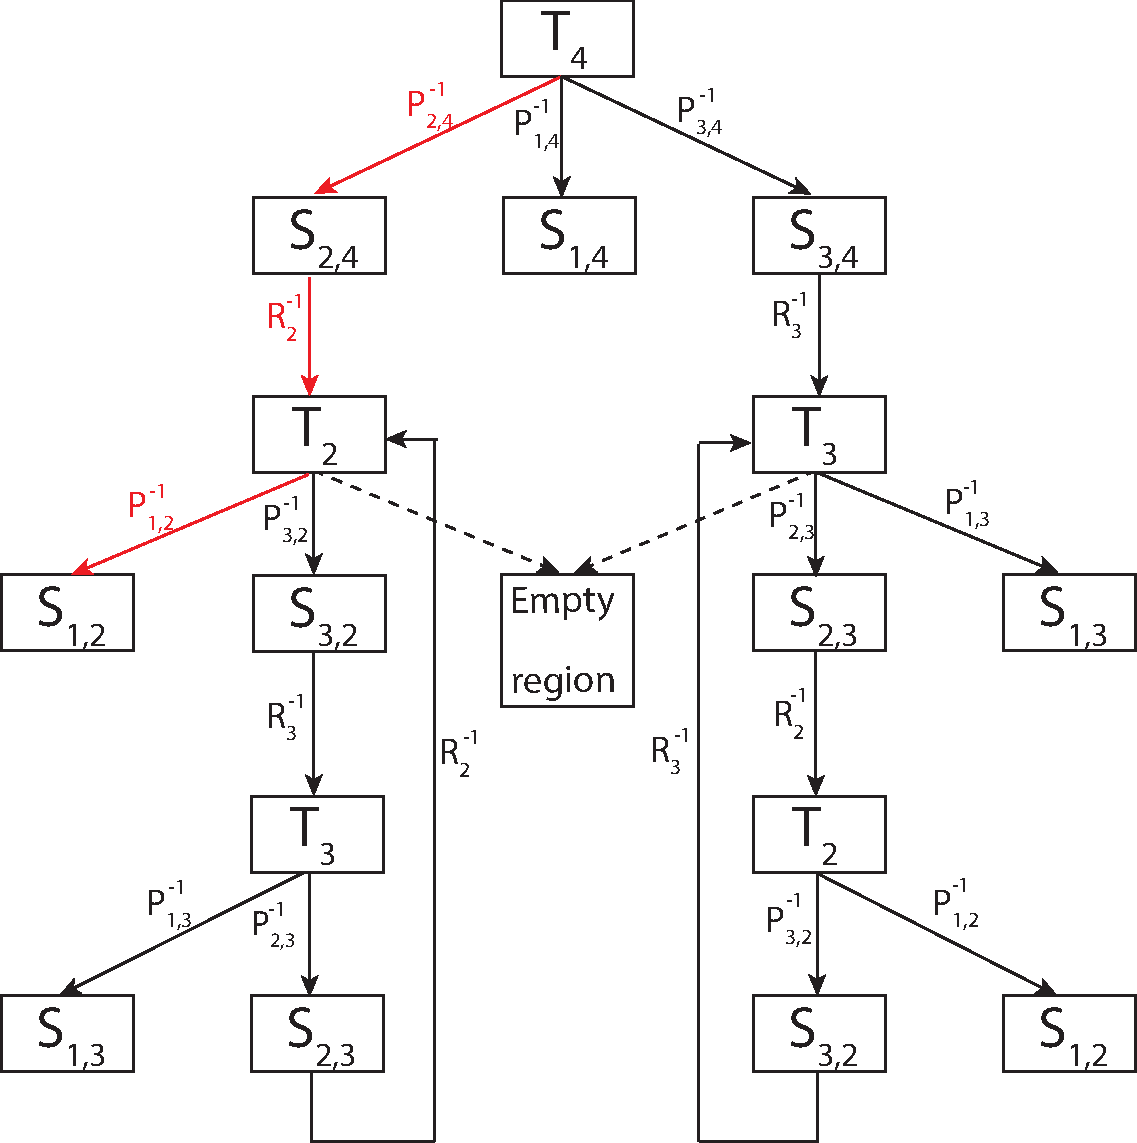
\includegraphics[width = \textwidth]{tree2}
\label{fig:tree}
  \end{center}
\caption{\textbf{Ray mapping tree.} It describes how to detect all the possible paths from \point{S} to \point{T}.}
\label{fig:tree}
\end{figure}
Using the procedure explained above, given a ray with coordinates
$(\variabile{q}, \variabile{p})\in \mbox{\set{T}{$4$}{}}$ we can establish whether it is located inside one of the positive luminance regions $\mbox{\set{R}{}{}}(\Pi)$ with or not.
In case the ray is inside a region $\mbox{\set{R}{}{}}(\Pi)$,
its corresponding coordinates $(\pos{s,}{$1$},\dir{s,}{$1$})\in \mbox{\set{S}{$1$}{}}$ are obtained using $\inversemap{M}{1,}{4}(\Pi)$, where $\Pi$ is the path followed by this ray. The luminance in Equation ($\ref{LT4}$) is, therefore, defined as in Equation (\ref{eq:PSluminance}), 
for some path $\Pi$ connecting \point{S}{}{} and \point{T}{}{}. The target intensity is calculated from Equation (\ref{I(eta)}). 
Indicating with $\variabile{q}^\textrm{\,min}(\Pi,\variabile{p})$ and $\variabile{q}^\textrm{\,max}(\Pi,\variabile{p})$ the minimum and maximum position coordinates of the intersection points between the boundaries $ \partial$\set{R}{}{}($\Pi$) and the line $\variabile{p}= \mbox{const}$,
Equation (\ref{I(eta)}) reduces to Equation (\ref{eta2}), if only two intersection points are found, and to Equation (\ref{eq:Ips}) in case more than two intersection points occur. For the two-faceted cup there are only two intersection points between a line $\dir{}{}{}=\mbox{const}$ and $\partial$\set{R}{}{}$(\Pi)$, hence, in this chapter we use Equation (\ref{eta2}).
We remark that, for a given ray with corresponding coordinates $(\pos{}{}, \dir{}{})$ on \set{T}{$4$}{}, only one path is possible as we are assuming that all lines are reflective.
Because of this, the regions \set{R}{}{}($\Pi$) do not overlap.
Next, the details of the procedure to compute the coordinates $\variabile{q}^\textrm{\,min}(\Pi, \variabile{p})$ and $\variabile{q}^\textrm{\,max}(\Pi, \variabile{p})$
are explained. 
\subsection{The structure of the backward ray mapping algorithm}\label{sec:algorithm_raymapping}
The goal is to determine the target intensity along a given direction $\variabile{p}=\const{const}$.
Also in the ray mapping method, we assume a Lambertian source, therefore the intensity is equal to the sum of the lengths of the line segments given by the intersection of the line $\variabile{p} = \mbox{const}$ and the support of $L$ (see Equation (\ref{eta2})).
To determine these line segments, a recursive procedure is developed.
The procedure starts on \set{T}{$4$}{} with a given direction $\variabile{p} = \mbox{const}$ and with the parallel rays corresponding to the end points $(\variabile{q}_{\ell}, \variabile{p}) = (-\variabile{b}, \variabile{p})$ and $(\variabile{q}_{\textrm{r}}, \variabile{p}) = (\variabile{b}, \variabile{p})$. 
We set the initial intensity $I(\variabile{p})=0$ along direction $\variabile{p} = \mbox{const}$. 
Considering the intersection between the line $\variabile{p}=\textrm{const}$ and the boundaries ($\partial$\set{T}{$4$,}{\lineai})$_{\lineai=1,2,3}$ three intervals are found.
Each interval corresponds to rays emitted by line $\lineai$ ($\lineai\in\{1,2,3\}$).
The rays corresponding to the end points of these intervals are traced back from \set{T}{$4$}{} to \set{T}{\lineai}{} where $\lineai$ is the line from which
they are emitted. Then, another interval of parallel rays along the corresponding direction in \set{T}{\lineai}{} has to be considered and the intersection points between the line $\dir{}{} = \dir{t,}{\lineai}$ and $\partial$\set{T}{\lineai,}{\lineaj} (with $\lineai\neq4$ and $\lineai\neq\lineaj$) are calculated, where $\dir{t,}{\lineai}$ is the new direction of the rays traced back.
The procedure continues recursively until the source is found. 
\\ \indent Before explaining the details, let us introduce some new notation. The role of the variables we introduce will become clear later on.
The coordinates in \set{T}{\lineaj}{} of the rays traced back from a line $\lineai\neq\lineaj$ to
line $\lineaj$ are indicated with $(\pos{t,}{\lineaj}^1, \dir{t,}{\lineaj})$ and $(\pos{t,}{\lineaj}^2, \dir{t,}{\lineaj})$.
The minimum and the maximum position coordinates are $\pos{t,}{\lineaj}^\textrm{\,min} = \min\{\pos{t,}{\lineaj}^1, \pos{t,}{\lineaj}^2\}$ and 
$\pos{t,}{\lineaj}^\textrm{\,max} = \max\{\pos{t,}{\lineaj}^1, \pos{t,}{\lineaj}^2\}$, respectively. The coordinates of the intersection points of
$\variabile{p}= \dir{t,}{\lineaj}$ with boundaries $\partial$\set{T}{\lineaj,}{\lineai} need to be determined for every $\lineai \in \{1,2,3\}$ and $\lineaj \in \{2,3,4\}$ with $\lineaj\neq\lineai$. 
They are indicated with  $(\variabile{u}_{\lineaj,\lineai}^\textrm{\,min}, \dir{t,}{\lineaj})$ and $(\variabile{u}_{\lineaj,\lineai}^\textrm{\,max}, \dir{t,}{\lineaj})$ where 
$\variabile{u}_{\lineaj,\lineai}^\textrm{\,min}<\variabile{u}_{\lineaj,\lineai}^\textrm{\,max}$. 
Since not all the rays whose corresponding coordinates are located inside the segment
$[\pos{t,}{\lineaj}^\textrm{\,min}, \pos{t,}{\lineaj}^\textrm{\,max}]$ with direction $ \dir{}{} =\dir{t,}{\lineaj}$ follow the same path, the intersection segment 
$[\variabile{v}_{\lineaj,\lineai}^\textrm{\,min}, \variabile{v}_{\lineaj,\lineai}^\textrm{\,max}] = [\pos{t,}{\lineaj}^\textrm{\,min}, \pos{t,}{\lineaj}^\textrm{\,max}] \cap [\variabile{u}_{\lineaj,\lineai}^\textrm{\,min}, \variabile{u}_{\lineaj,\lineai}^\textrm{\,max}]$ needs to be calculated. $(\variabile{v}_{\lineaj,\lineai}^\textrm{\,min},\dir{t,}{\lineaj})$ and $(\variabile{v}_{\lineaj,\lineai}^\textrm{\,max},\dir{t,}{\lineaj})$ are the coordinates of the rays that need to be traced back from line $\lineaj$ to line $\lineai$.
\\ \indent The method can be outlined as follows.
\begin{enumerate}
\item Calculate the intersection points $(\variabile{u}_{4,\lineai}^\textrm{\,min}, \variabile{p})$ and $(\variabile{u}_{4,\lineai}^\textrm{\,max}, \variabile{p})$ between line $\variabile{p}= \const{const.}$ and $\partial$\set{T}{$4$,}{\lineai} for every $\lineai\in\{1,2,3\}$, where $\variabile{u}_{4,\lineai}^\textrm{\,min}<\variabile{u}_{4,\lineai}^\textrm{\,max}$. This can be done analytically because the exact expression of the boundaries $\partial$\set{T}{$4$,}{\lineai} is found as explained in Section \ref{sec:cup_raymapping}.
\item Calculate the intersection segment 
\begin{equation*}
[\variabile{v}_{4, \lineai}^\textrm{\,min}, \variabile{v}_{4, \lineai}^\textrm{\,max}] = [\variabile{u}_{4, \lineai}^\textrm{\,min}, \variabile{u}_{4, \lineai}^\textrm{\,max}]\cap
 [\pos{}{}^\textrm{\,min}, \pos{}{}^\textrm{\,max}].
\end{equation*}
\item If $\lineai= 1$, the coordinates $(\variabile{v}_{4,1}^\textrm{\,min}, \variabile{p})$ and $(\variabile{v}_{4,1}^\textrm{\,max}, \variabile{p})$ equal the coordinates $(\variabile{q}^\textrm{\,min}(\Pi, \variabile{p}), \variabile{p})$ and $(\variabile{q}^\textrm{\,max}(\Pi, \variabile{p}), \variabile{p})$ of the rays located on the boundary $\partial$\set{R}{}{}$(\Pi)$ with $\Pi = (1,4)$. All the parallel rays with direction coordinate $\variabile{p}$ and $\variabile{q}$-position coordinate $\variabile{u}_{4,1}^\textrm{\,min}\leq \variabile{q} \leq \variabile{u}_{4,1}^\textrm{\,max}$ are emitted by the source and they directly hit the target. Update the intensity using (\ref{eta2}):
\begin{equation*}
I(\variabile{p})= I(\variabile{p})+\variabile{q}^\textrm{\,max}(\Pi, \dir{}{})-\variabile{q}^\textrm{\,min}(\Pi, \dir{}{}).
\end{equation*}
\item If $\lineai\neq 1$, continue with the following steps
\item Trace back $(\variabile{v}_{4,\lineai}^\textrm{\,min}, \variabile{p})$ and $(\variabile{v}_{4,\lineai}^\textrm{\,max}, \variabile{p})$ from line $4$ to line $\lineai$ to find their corresponding coordinates on \set{T}{\lineai}{}:
\begin{equation*}
\begin{aligned}
(\pos{t,}{\lineai}^{\,1}, \dir{t,}{\lineai})& =\inversemap{R}{\lineai}{}\circ \inversemap{P}{\lineai,}{4}(\variabile{v}_{4,\lineai}^\textrm{\,min}, \variabile{p}),  \\
(\pos{t,}{\lineai}^{\,2}, \dir{t,}{\lineai}) & =\inversemap{R}{\lineai}{}\circ \inversemap{P}{\lineai,}{4}(\variabile{u}_{4,\lineai}^\textrm{\,max}, \variabile{p}).
\end{aligned}
\end{equation*}
\item Update the path $\Pi = (\lineai, 4)$
\item Determine $\pos{t,}{\lineai}^\textrm{\,min}= \min\{\pos{t,}{\lineai}^{\,1}, \pos{t,}{\lineai}^{\,2}\}$ and $\pos{t,}{\lineai}^\textrm{\,max}= \max\{\pos{t,}{\lineai}^{\,1}, \pos{t,}{\lineai}^{\,2}\}$
\item Calculate the intersection points $(\variabile{u}_{\lineai,\lineaj}^\textrm{\,min}, \variabile{p})$ and $(\variabile{u}_{\lineai,\lineaj}^\textrm{\,max}, \variabile{p})$ between the line $\dir{}{}=\dir{t,}{\lineai}$ and 
$\partial$\set{T}{\lineai,}{\lineaj} for every $\lineaj\in\{1,2,3\}$ with $\lineaj\neq\lineai$.
\item Since not all rays whose corresponding coordinates are located inside the segment
$[\pos{t,}{\lineai}^\textrm{\,min}, \pos{t,}{\lineai}^\textrm{\,max}]$ follow the same path,
 compute the intersection segment 
\begin{equation*}
[\variabile{v}_{\lineai, \lineaj}^\textrm{\,min}, \variabile{v}_{\lineai, \lineaj}^\textrm{\,max}] = [\variabile{u}_{\lineai, \lineaj}^\textrm{\,min}, \variabile{u}_{\lineai, \lineaj}^\textrm{\,max}]\cap
 [\pos{t,}{\lineai}^\textrm{\,min}, \pos{t,}{\lineai}^\textrm{\,max}]
\end{equation*}
\item If $\lineaj\neq 1$ 
\begin{itemize}
\item[a)] Trace back $(\variabile{v}_{\lineai, \lineaj}^\textrm{\,min}, \dir{t,}{\lineai})$ and $(\variabile{v}_{\lineai, \lineaj}^\textrm{\,max}, \dir{t,}{\lineai})$ from $\lineai$ to $\lineaj$ 
\begin{equation*}
\begin{aligned}
(\pos{t,}{\lineaj}^{\,1}, \dir{t,}{\lineaj})& =\inversemap{R}{\lineaj}{}\circ \inversemap{P}{\lineaj,}{\lineai}(\variabile{v}_{\lineai, \lineaj}^\textrm{\,min}, \dir{t,}{\lineai}),  \\
(\pos{t,}{\lineaj}^{\,2}, \dir{t,}{\lineaj}) & =\inversemap{R}{\lineaj}{}\circ \inversemap{P}{\lineaj,}{\lineai}(\variabile{v}_{\lineai, \lineaj}^\textrm{\,max}, \dir{t,}{\lineai}).
\end{aligned}
\end{equation*}
\item[b)] Update the path: $\Pi = (\lineaj, \Pi)$
\item[c)] Set $\lineai=\lineaj$ and repeat the procedure from point $7$.
\end{itemize}
Else if $\lineaj=1$, the rays reached the source and a possible path $\Pi = (1, \cdots, 4)$ is found. 
\begin{itemize}
\item[a)]
Trace back to source
\begin{equation*}
\begin{aligned}
(\pos{s,}{$1$}^{\,1}, \dir{s,}{$1$})& = \inversemap{P}{1,}{\lineai}(\variabile{v}_{\lineai, 1}^\textrm{\,min}, \dir{t,}{\lineai}),  \\
(\pos{s,}{$1$}^{\,2}, \dir{s,}{$1$}) & =\inversemap{P}{1,}{\lineai}(\variabile{v}_{\lineai, 1}^\textrm{\,max}, \dir{t,}{\lineai}).
\end{aligned}
\end{equation*}
\item[b)] Apply the forward map
\begin{equation*}
\begin{aligned}
 (\pos{}{}^{1}(\Pi, \dir{}{}), \dir{}{})&= \mapnumb{M}_{1,4}(\Pi)(\pos{s,}{$1$}^{\,1}, \dir{s,}{$1$}),\\
 (\pos{}{}^{2}(\Pi, \dir{}{}), \dir{}{})&= \mapnumb{M}_{1,4}(\Pi)(\pos{s,}{$1$}^{\,2}, \dir{s,}{$1$}).
\end{aligned}
\end{equation*}
\item[c)] Update the intensity: $$I(\variabile{p}) = I(\variabile{p})+\pos{}{}^{\textrm{max}}(\Pi, \dir{}{})- \pos{}{}^{\textrm{min}}(\Pi, \dir{}{})$$
where 
$\pos{}{}^\textrm{min}(\Pi, \dir{}{}) := \pos{}{}^\textrm{min} =\min\{ \pos{}{}^{1}(\Pi, \dir{}{}), \pos{}{}^{2}(\Pi, \dir{}{})\}$ \\ and $\quad\pos{}{}^\textrm{max}(\Pi, \dir{}{}) := \pos{}{}^\textrm{max} =\max\{\pos{}{}^{1}(\Pi, \dir{}{}), \pos{}{}^{2}(\Pi, \dir{}{})\}.$
\end{itemize}
\end{enumerate}
\indent
To clarify the method, we give an example that describes how the target intensity along direction $\variabile{p}= -0.2$ is calculated.
From Figure $\ref{fig:T41}$ to Figure $\ref{fig:T43}$ the steps used in this example are shown.
A detailed description of those figures is given in the following.
\\ \indent The procedure starts with the rays with direction $\variabile{p} = 0.2$ on \set{T}{$4$}{}, where $\variabile{q}_\ell= -\variabile{b}$ and
$\variabile{q}_\textrm{r}= \variabile{b}$ are the left and the right end points of the target \point{T}, respectively.
 The intersection points $(\variabile{u}_{4,\lineai}^\textrm{\,min}, \variabile{p})$ and
$(\variabile{u}_{4,\lineai}^\textrm{\,max}, \variabile{p})$
of the line $\variabile{p}= -0.2$
 with boundaries $\partial\mbox{\set{T}{$4$,}{\lineai}}$ are computed for every $\lineai\neq 4$. \\ \indent
We start from $\lineai=1$. Therefore the coordinates  $(\variabile{u}_{4,1}^\textrm{\,min}, \variabile{p})$ and
$(\variabile{u}_{4,1}^\textrm{max}, \variabile{p})$ of the intersection points between line $\variabile{p} = -0.2$ and the boundary $\partial\mbox{\set{T}{$4$,}{$1$}}$ are computed and these points are depicted in Figure \ref{fig:T41}.
 The source is now reached because $\lineai = 1$ and, one possible path is found.
 The points $(\variabile{u}_{4,1}^\textrm{\,min}, \variabile{p})$
and $(\variabile{u}_{4,1}^\textrm{\,max}, \variabile{p})$ are located on the boundaries of the region formed by the rays that leave the source and directly hit the target, that is the rays located on
$\partial \mbox{\set{R}{}{}}(\Pi_1)$ with $\Pi_1 = (1,4)$.
Therefore, the contribution to the intensity formed by the rays that follow the path $\Pi_1 = (1,4)$ is given by 
$\variabile{u}_{4,1}^\textrm{\,max}-\variabile{u}_{4,1}^\textrm{\,min}$. \\ \indent
We continue with $\lineai = 2$. 
The boundary $\partial\mbox{\set{T}{$4$,}{$2$}}$ is considered in order to find other paths.
The intersection points $(\variabile{u}_{4,2}^\textrm{\,min}, \variabile{p})$ and
$(\variabile{u}_{4,2}^\textrm{\,max}, \variabile{p})$ of line
$\variabile{p}=-0.2$ with the boundary
$\partial\mbox{\set{T}{$4$,}{$2$}}$ are calculated.
They are depicted in Figure \ref{fig:T42} with the magenta dots. Also the intersection segment 
\begin{equation}
[\variabile{v}_{4,2}^\textrm{\,min}, \variabile{v}_{4,2}^\textrm{\,max}] = [\variabile{u}_{4,2}^\textrm{\,min}, \variabile{u}_{4,2}^\textrm{\,max}]\cap [\variabile{q}^\textrm{min}, \variabile{q}^\textrm{max}]
\end{equation}
is calculated. In \set{T}{$4$}{} $\variabile{v}_{4,2}^\textrm{\,min} = \variabile{u}_{4,2}^\textrm{\,min}$ and $\variabile{v}_{4,2}^\textrm{\,max} = \variabile{u}_{4,2}^\textrm{\,max}$ because $\variabile{q}^\textrm{min} = -\variabile{b}$ and $\variabile{q}^\textrm{max} = \variabile{b}$ always coincide with the end points of \set{T}{$4$}{}.
Their corresponding position coordinates $\pos{s,}{$2$}^1$ and $\pos{s,}{$2$}^2$ on \set{S}{$2$}{}
are obtained from:
\begin{equation}\label{inverseP}
\begin{split}
 \inversemap{P}{2,}{4}
(\variabile{v}_{4,2}^\textrm{\,min}, \variabile{p}) &=  (\pos{s,}{$2$}^1, \dir{s,}{$2$}^1), \\
 \inversemap{P}{2,}{4}
(\variabile{v}_{4,2}^\textrm{\,max}, \variabile{p}) &=  (\pos{s,}{$2$}^2, \dir{s,}{$2$}^2).
\end{split}
\end{equation}
 The directions
$\dir{s,}{$2$}^1$ and $\dir{s,}{$2$}^2 $ on \set{S}{$2$}{}
are given considering the direction $\dir{t,}{$2$} = \dir{}{}$ with respect to the normal
$\boldsymbol{\nu}_{2}$ of line $2$.
 Note that $\dir{s,}{$2$}^1=\dir{s,}{$2$}^2$ because all the lines are straight lines, their normals do not depend on the position where it is computed. Thus, in the following we will omit the subscripts for the direction coordinates.
 Then, the corresponding direction $\dir{t,}{$2$}^1=\dir{t,}{$2$}^2$ on \set{T}{$2$}{}
 is calculated from:
\begin{equation}\label{inverseR}
\begin{split}
\inversemap{R}{2}{}(\pos{s,}{$2$}^1, \dir{s,}{$2$}) &= (\pos{t,}{$2$}^1, \dir{t,}{$2$}), \\
\inversemap{R}{2}{}(\pos{s,}{$2$}^2, \dir{s,}{$2$}) &= (\pos{t,}{$2$}^2, \dir{t,}{$2$}).
\end{split}
\end{equation}
Note that $\pos{s,}{$2$}^1 = \pos{t,}{$2$}^1$ and $\pos{s,}{$2$}^2= \pos{t,}{$2$}^2$ since the reflection map does not change the position coordinates.
 Equations (\ref{inverseP}) and (\ref{inverseR}) lead to: \begin{equation}
\begin{split}
\inversemap{R}{2}{}\circ \inversemap{P}{2,}{4}(\variabile{v}_{4,2}^\textrm{\,min}, \variabile{p}) &= (\pos{t,}{$2$}^1, \dir{t,}{$2$}),\\
\inversemap{R}{2}{}\circ \inversemap{P}{2,}{4}(\variabile{v}_{4,2}^\textrm{\,max}, \variabile{p}) &= (\pos{t,}{$2$}^2, \dir{t,}{$2$}).
\end{split}
\end{equation} The map $\inversemap{R}{2}{}\circ \inversemap{P}{2,}{4}$  is depicted in red in Figure \ref{fig:tree}.
The minimum 
 $\pos{t,}{$2$}^\textrm{\,min} = \min\{\pos{t,}{$2$}^1, \pos{t,}{$2$}^2\}$ and maximum
 $\pos{t,}{$2$}^\textrm{\,max} = \max\{\pos{t,}{$2$}^1, \pos{t,}{$2$}^2\}$ are calculated. The points with coordinates  $(\pos{t,}{$2$}^\textrm{\,min}, \dir{t,}{$2$})$  and  $(\pos{t,}{$2$}^\textrm{\,max}, \dir{t,}{$2$})$  are depicted in blue Figure \ref{fig:T21}, where $\dir{t,}{$2$}=0.82$.
 To verify whether the corresponding rays are illuminated or not by the source, the procedure used for
 \set{T}{$4$}{} is now applied to \set{T}{$2$}{}
 along direction $\dir{t,}{$2$}=0.82$. \\ \indent
  Next, the intersection points $(\variabile{u}_{2,\lineai}^\textrm{\,min}, \dir{t,}{$2$})$ and
$(\variabile{u}_{2,\lineai}^\textrm{\,max}, \dir{t,}{$2$})$
of line $\dir{t,}{$2$}= 0.82$
 with boundaries $\partial\mbox{\set{T}{$2$,}{\lineai}}$ are computed for every $\lineai\in\{1,3\}.$
 We start from the boundary $\partial$\set{T}{$2$,}{$1$} obtaining the points $(\variabile{u}_{2, 1}^\textrm{\,min}, \dir{t,}{$2$})$ and
 $(\variabile{u}_{2, 1}^\textrm{\,max}, \dir{t,}{$2$})$ shown in Figure \ref{fig:T21}.
 Now, the position coordinates $\variabile{v}_{2, 1}^\textrm{\,min} = \max\{\pos{t,}{$2$}^ \textrm{\,min},\variabile{u}_{2,1}^\textrm{\,min}\}$
 and $\variabile{v}_{2, 1}^\textrm{\,max} = \min\{\pos{t,}{$2$}^ \textrm{\,max},\variabile{u}_{2, 1}^\textrm{\,max}\}$ need to be determined.
 All the rays located inside the segment $[\variabile{v}_{2, 1}^\textrm{\,min},\variabile{v}_{2, 1}^\textrm{\,max}]$ in
  \set{T}{$2$}{} and with direction $\dir{t,}{$2$}$ follow path $\Pi_2 = (1,2,4)$. In particular, the rays corresponding to the coordinates $(\variabile{v}_{2, 1}^\textrm{\,min},\dir{t,}{$2$} )$ and $(\variabile{v}_{2, 1}^\textrm{\,max},\dir{t,}{$2$} )$ are  located on the boundaries of the region \set{R}{}{}$(\Pi_2)$ on \set{T}{$4$}{}
  formed by all the rays that follow path $\Pi_2$.
  Their corresponding coordinates $(\variabile{q}^{1}(\Pi_2, \variabile{p}), \variabile{p})$ and
 $(\variabile{q}^{2}(\Pi_2, \variabile{p}), \variabile{p})$ on \set{T}{$4$}{} are obtained from:\footnote{With a slight abuse of notation we indicate  $\variabile{q}^{1}(\Pi, \variabile{p})$ with $\variabile{q}^{1}$ and 
$ \variabile{q}^{2}(\Pi, \variabile{p})$ with $\variabile{q}^{2}$.}
\begin{equation}
\begin{split}
\mapnumb{P}_{2,4} \circ \mapnumb{R}_{2} (\variabile{v}_{2, 1}^\textrm{\,min},\dir{t,}{$2$} ) & = (\variabile{q}^{1}, \variabile{p}), \\
\mapnumb{P}_{2,4} \circ \mapnumb{R}_{2} (\variabile{v}_{2, 1}^\textrm{\,max},\dir{t,}{$2$} ) & = (\variabile{q}^{2}, \variabile{p}).
\end{split}
\end{equation} 
The rays corresponding to the coordinates $(\variabile{q}^{1}, \variabile{p})$ and $(\variabile{q}^{2}, \variabile{p})$ are located
 on the boundary $\partial$\set{R}{}{}$(\Pi_2)$ along direction $\variabile{p}=-0.2$.
Indicating with $\variabile{q}^{\textrm{min}} = \min\{\variabile{q}^{1}, \variabile{q}^2\}$ and $\variabile{q}^{\textrm{max}} = \max\{\variabile{q}^{1}, \variabile{q}^2\}$, the distance $\variabile{q}^{\textrm{max}}-\variabile{q}^{\textrm{min}}$ gives the contribution to the intensity $I(\variabile{p})$ of the rays located in \set{R}{}{}$(\Pi_2)$ where $\variabile{p}=-0.2$.\\
\indent  \set{T}{$2$}{} can also be illuminated by line $3$, therefore the intersection points $(\variabile{u}_{2, 3}^\textrm{\,min}, \dir{t,}{$2$})$ and $(\variabile{u}_{2, 3}^\textrm{\,max}, \dir{t,}{$2$})$ of line
 $\dir{t,}{$2$}=0.82$ and $\partial \mbox{\set{T}{$2$,}{$3$}}$ are calculated, these points are depicted in Figure \ref{fig:T22}.
 The coordinates $(\variabile{v}_{2, 3}^\textrm{\,min}, \dir{t,}{$2$})$ and $(\variabile{v}_{2, 3}^\textrm{\,max}, \dir{t,}{$2$})$ are shown in the same figure.
 As the source is not reached yet ($\lineai=3$), the rays corresponding to $(\variabile{v}_{2, 3}^\textrm{\,min}, \dir{t,}{$2$})$ and $(\variabile{v}_{2, 3}^\textrm{\,max}, \dir{t,}{$2$})$ are followed back using the inverses of the propagation and the reflection maps. The coordinates on \set{T}{$3$}{} are shown  with blue circles in Figure \ref{fig:T31} and they are obtained from:
 \begin{equation}
\begin{split}
\inversemap{R}{3}{}\circ \inversemap{P}{3,2}{}(\variabile{v}_{2, 3}^\textrm{\,min}, \dir{t,}{$2$}) &= (\pos{t,}{$3$}^{1}, \dir{t,}{$3$}),\\
\inversemap{R}{3}{}\circ \inversemap{P}{2,3}{}(\variabile{v}_{2, 3}^\textrm{\,max}, \dir{t,}{$2$}) &= (\pos{t,}{$3$}^{2}, \dir{t,}{$3$}).
\end{split}
\end{equation}
The minimum and the maximum position coordinates are $\pos{t,}{$3$}^{\textrm{min}}= \min\{\pos{t,}{$3$}^{1}, \pos{t,}{$3$}^{2}\}$ and 
$\pos{t,}{$3$}^{\textrm{max}}= \max\{\pos{t,}{$3$}^{1}, \pos{t,}{$3$}^{2}\}$, respectively.
We found that $\variabile{v}_{3,2}^\textrm{max}\neq\variabile{u}_{3,2}^\textrm{max}$ because $[\pos{t,}{$3$}^\textrm{min}, \pos{t,}{$3$}^\textrm{max}]\subset
[\variabile{u}_{3,2}^\textrm{min},\variabile{u}_{3,2}^\textrm{max}]$, this means that the rays with corresponding position coordinates inside the interval 
$[\pos{t,}{$3$}^\textrm{max},\variabile{u}_{3,2}^\textrm{max}]$ will follow a different path. 
The procedure continues recursively.
  It stops either when the ray encounters the source, i.e., when $\lineai=1$, or when no intersection points between the
  direction $\variabile{p}=\dir{t,}{\lineaj}$ and the boundaries $\partial$\set{T}{\lineaj,}{\lineai} are determined for any $\lineai\in{1,2,3}$ with $\lineai\neq\lineaj$. \\ \indent
  If the source is reached, then a valid path $\Pi = (1,3,2,4)$ is found. Using the inverse of the propagation map, we compute
\begin{equation}
\begin{aligned}
\inversemap{P}{1,3}{}(\pos{t,}{$3$}^\textrm{min}, \dir{t,}{$3$}) = (\pos{s,}{$1$}^1, \dir{s,}{$1$}), \\ 
\inversemap{P}{1,3}{}(\pos{t,}{$3$}^\textrm{max}, \dir{t,}{$3$}) = (\pos{s,}{$1$}^2, \dir{s,}{$1$}).
 \end{aligned}
\end{equation} 
The forward map $\mapnumb{M}_{1,4}(\Pi)$:\set{S}{$1$}{}$\rightarrow$\set{R}{}{}$(\Pi)$ restricted to path $\Pi = (1,3,2,4)$, i.e.
\begin{equation}
\mapnumb{M}_{1,4} = \mapnumb{P}_{2,4}\circ\mapnumb{R}_{2}\circ\mapnumb{P}_{3,2}\circ\mapnumb{R}_{3}\circ\mapnumb{P}_{1,3}
\end{equation}
is applied to the coordinates $(\pos{s,}{$1$}^{1}, \dir{s,}{$1$})$ and $(\pos{s,}{$1$}^{1}, \dir{s,}{$1$})$:
\begin{equation}
\begin{split}
\mapnumb{M}_{1,4}(\pos{s,}{$1$}^{1}, \dir{s,}{$1$}) &= (\variabile{q}^{1}(\Pi, \variabile{p}), \variabile{p}),\\
\mapnumb{M}_{1,4}(\pos{s,}{$1$}^{2}, \dir{s,}{$1$}) &= (\variabile{q}^{2}(\Pi, \variabile{p}), \variabile{p}).
\end{split}
\end{equation} 
The coordinates $(\variabile{q}^{1}, \variabile{p}):=(\variabile{q}^{1}(\Pi, \variabile{p}), \variabile{p})$ and
  $(\variabile{q}^{2}, \variabile{p}):=(\variabile{q}^{2}(\Pi, \variabile{p}), \variabile{p})$ located on $\partial$\set{R}{}{}$(\Pi)$ in \set{T}{$4$}{} are found.
Indicating with $\variabile{q}^{\textrm{min}}= \min\{\variabile{q}^{1}, \variabile{q}^{2}\}$ and $\variabile{q}^{\textrm{max}}= \max\{\variabile{q}^{1}, \variabile{q}^{2}\}$, the contribution to the intensity due to the rays that follow path $\Pi$ is given by:
\begin{equation}
I(\variabile{p}) = I(\variabile{p})+\variabile{q}^{\textrm{max}}(\Pi, \variabile{p})-\variabile{q}^{\textrm{min}}(\Pi, \variabile{p}). 
\end{equation}
  If no intersection points are found, then the rays traced are
  not emitted by the source, therefore no contribution to the intensity needs to be added. This is, for instance, the case for rays with
  coordinates $(\variabile{v}_{2, 3}^\textrm{\,min}, 0.82)$ and $(\variabile{v}_{2, 3}^\textrm{\,max}, 0.82)$
  on \set{T}{$2$}{} in Figure \ref{fig:T22}. Below we explain this case in detail. \\ \indent
  In Figure \ref{fig:T31}, the coordinates $(\pos{t,}{$3$}^{\textrm{min}}, \dir{t,}{$3$})$ and $(\pos{t,}{$3$}^{\textrm{max}}, \dir{t,}{$3$})$ in \set{T}{$3$}{} with $\dir{t,}{$3$}=-0.29$ are shown.
  They are obtained from:
\begin{equation}
\begin{split}
 \inversemap{R}{3}{}\circ\inversemap{P}{3,}{2}(\variabile{v}_{2, 3}^\textrm{\,min}, 0.82)& = (\pos{t,}{$3$}^{1}, \dir{t,}{$3$}),\\
\inversemap{R}{3}{}\circ\inversemap{P}{3,}{2}(\variabile{v}_{2, 3}^\textrm{\,max}, 0.82)& = (\pos{t,}{$3$}^{2}, \dir{t,}{$3$}).
\end{split}
\end{equation}
 From Figure \ref{fig:T31} we note that there are no intersection points of the line $\dir{t,}{$3$}=-0.29$ with $\partial\mbox{\set{T}{$3$,}{$1$}}$.
  So, only the coordinates of the intersections $(\variabile{u}_{3, 2}^\textrm{\,min}, -0.29)$ and $(\variabile{u}_{3, 2}^\textrm{\,max}, -0.29)$ between line $\dir{t,}{$3$}=-0.29$ and  $\partial\mbox{\set{T}{$3$,}{$2$}}$ are calculated.
  Next, the intersection interval 
\begin{equation}
[\variabile{v}_{3, 2}^\textrm{\,min},\variabile{v}_{3, 2}^\textrm{\,max}] = [\variabile{u}_{3, 2}^\textrm{\,min}, \variabile{u}_{3, 2}^\textrm{\,max}] \cap [\pos{t,}{$3$}^{\textrm{min}}, \pos{t,}{$3$}^{\textrm{max}}],
\end{equation} formed by parallel rays with direction $\dir{t,}{$3$} = -0.29$, is considered.
  Using
\begin{equation}
\begin{split}
 \inversemap{R}{2}{}\circ\inversemap{P}{2,}{3}(\variabile{v}_{3, 2}^\textrm{\,min},-0.29) & = (\pos{t,}{$2$}^{\textrm{min}}, \dir{t,}{$2$}),\\
 \inversemap{R}{2}{}\circ\inversemap{P}{2,}{3}(\variabile{v}_{3, 2}^\textrm{\,max},-0.29) & = (\pos{t,}{$2$}^{\textrm{max}}, \dir{t,}{$2$}),\\
\end{split}
\end{equation}
  the corresponding coordinates $(\pos{t,}{$2$}^{\textrm{max}}, \dir{t,}{$2$})$ and $(\pos{t,}{$2$}^{\textrm{min}}, \dir{t,}{$2$})$ on \set{T}{$2$}{} are found (see Figure \ref{fig:T23})
  with $\dir{t,}{$2$}=-0.41$.
  Now the procedure is repeated again for \set{T}{$2$}{} along the direction $\dir{t,}{$2$}$.
  No intersection points between the line $\dir{t,}{$2$}=-0.41$ and $\partial$\set{T}{$2$,}{$1$} occur. 
Only, the intersection points $(\variabile{u}_{2,3}^\textrm{\,min},\dir{t,}{$2$})$ and $(\variabile{u}_{2,3}^\textrm{\,max},\dir{t,}{$2$})$
  of line $\dir{t,}{$2$}=-0.41$ and $\partial$\set{T}{$2$,}{$3$} are found.
  The intersection segment 
\begin{equation}
[\variabile{v}_{2,3}^\textrm{\,min},\variabile{v}_{2,3}^\textrm{\,max}] = [\variabile{u}_{2,3}^\textrm{\,min},\variabile{u}_{2,3}^\textrm{\,max}] \cap  [\pos{t,}{$2$}^\textrm{\,min},\pos{t,}{$2$}^\textrm{\,max}]
\end{equation}
is calculated. 
The coordinates on \set{T}{$3$}{} corresponding to the end points of the intersection interval are found using:
\begin{equation}
\begin{split}
\inversemap{R}{3}{}\circ\inversemap{P}{3,}{2} (\variabile{v}_{2,3}^\textrm{\,min},\dir{t,}{$2$})& = (\pos{t,}{$3$}^\textrm{\,min},\dir{t,}{$3$}),\\
\inversemap{R}{3}{}\circ\inversemap{P}{3,}{2} (\variabile{v}_{2,3}^\textrm{\,max},\dir{t,}{$2$})& = (\pos{t,}{$3$}^\textrm{\,max},\dir{t,}{$3$}),
\end{split}
\end{equation}  where $ \dir{t,}{$3$} = 0.91$ (see Figure \ref{fig:T32}). \\ \indent
 Considering the PS \set{T}{$3$}{} and the direction $\dir{t,}{$3$}=0.91$, we note that there are no intersection points of line
 $\dir{t,}{$3$}=0.91$ with both $\partial$\set{T}{$3$,}{$1$} and $\partial$\set{T}{$3$,}{$2$}.
 Indeed, the whole segment $[\pos{t,}{$3$}^\textrm{\,min},\pos{t,}{$3$}^\textrm{\,max}]$ is outside both
 \set{T}{$3$,}{$2$} and \set{T}{$3$,}{$1$}. Because of this, all the rays with $\variabile{q}$-coordinates inside the interval
 $[\pos{t,}{$3$}^\textrm{\,min},\pos{t,}{$3$}^\textrm{\,max}]$
and with direction $\variabile{p}= \dir{t,}{$3$}$ are not illuminated by the source and no new real path is found.
\\ \indent
Finally, the recursive procedure is applied to \set{T}{$4$,}{$3$}.
The first step is depicted in Figure \ref{fig:T43}.
 We decided not to show all the steps for \set{T}{$4$,}{$3$} as they are similar to those used for \set{T}{$4$,}{$2$} and explained above.
 \\ \indent Finally, to compute the intensity along another direction $\variabile{p}^{\variabile{h}}\in[-1,1]$ on \set{T}{$4$}{},
the procedure explained for $\variabile{p}=-0.2$ is repeated for $\variabile{p}= \variabile{p}^{\variabile{h}}$.
In this way we find all the possible paths $\Pi$ and the positive luminance regions \set{R}{}{}$(\Pi)$ on \set{T}{$4$}{}.
Furthermore, considering every time the coordinates located on the boundaries of the regions \set{T}{\lineai,}{\lineaj} for every $\lineaj\neq\lineai$, also the boundaries $\partial$\set{R}{}{}$(\Pi)$ are determined for a given path $\Pi$ as well as the coordinates $\variabile{q}^\textrm{\,min}(\Pi,\variabile{p})$ and $\variabile{q}^\textrm{\,max}(\Pi,\variabile{p})$ for every $\variabile{p}\in [-1,1]$.
In Algorithm \ref{alg}, the main steps to calculate the intensity $I(\variabile{p})$ along a direction
$\variabile{p} = \variabile{p}^{\variabile{h}}$ in \set{T}{$4$}{} are given, where for the first step we take $\lineaj=4$.
\begin{figure}
\begin{minipage}[t]{.48\textwidth}
\centering
   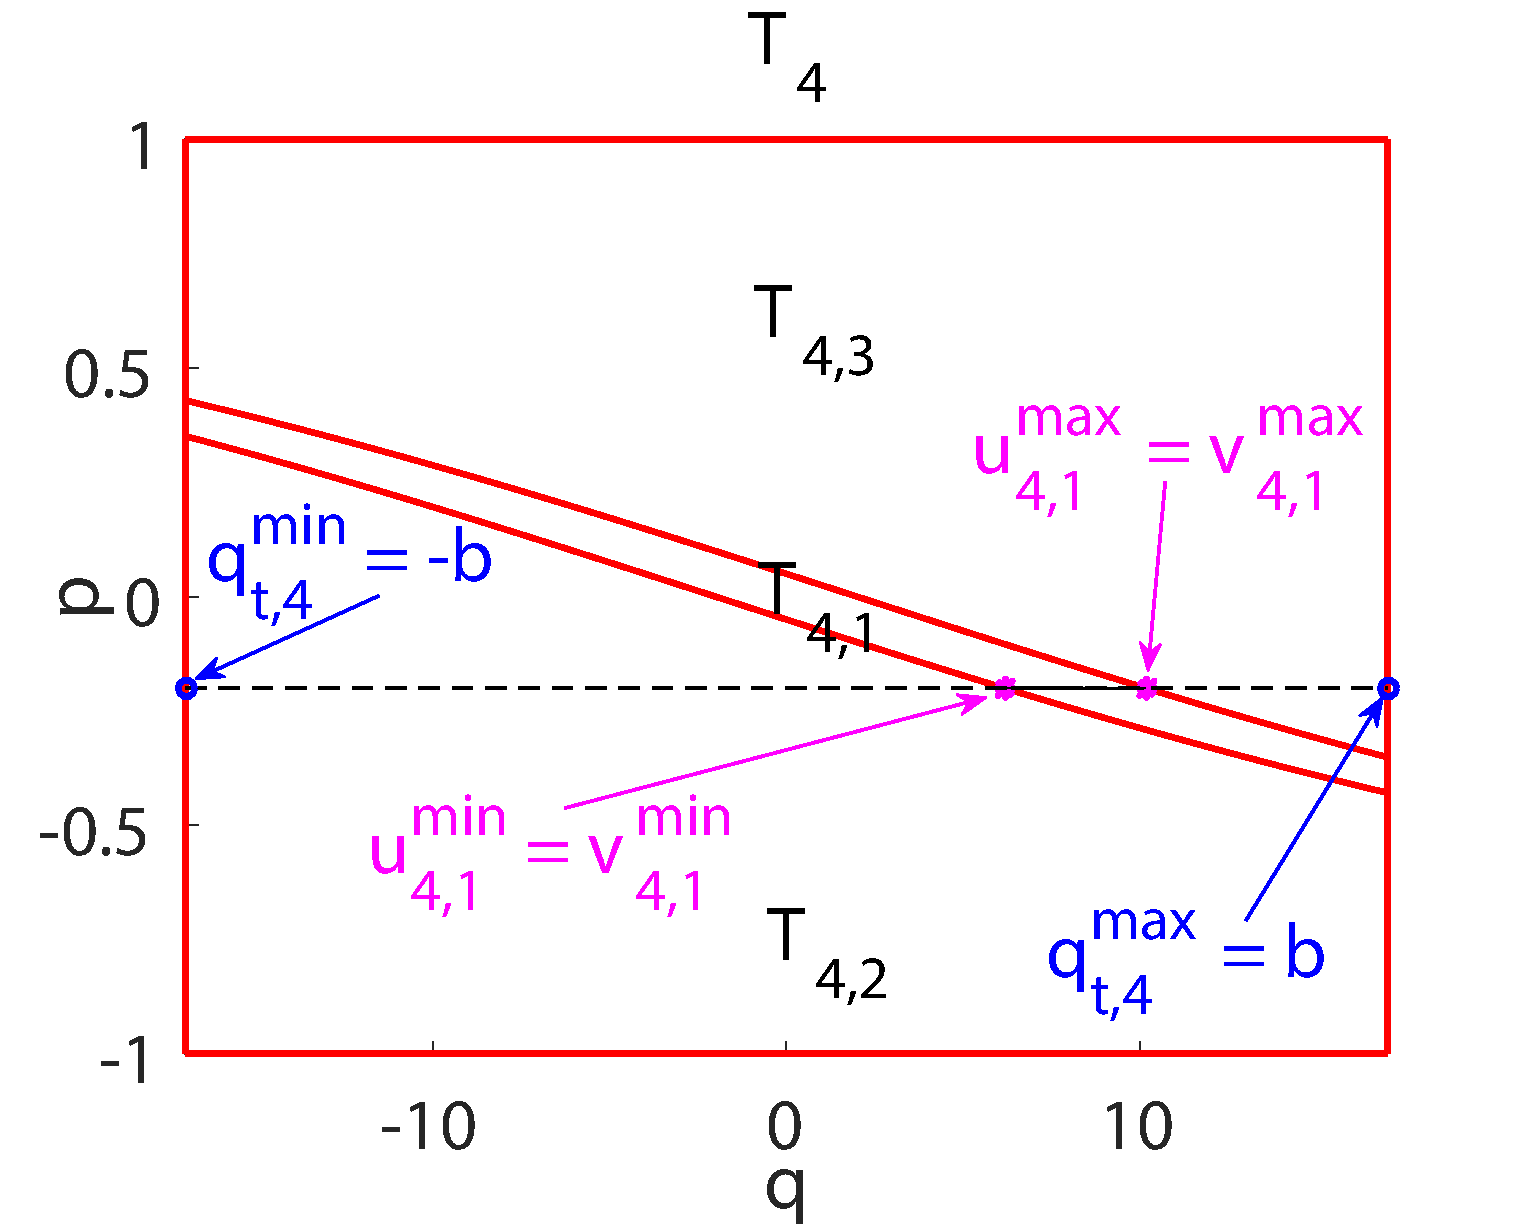
\includegraphics[width=\textwidth]{T4_1}
  \caption{\footnotesize{\textbf{Target PS of line $4$.} $\pos{t,}{$4$}^{\textrm{min}}$ and $\pos{t,}{$4$}^{\textrm{max}}$ are the $\variabile{x}$-coordinates of the end points of line $4$.
  The intersection points between the line $\variabile{p} = -0.2$ and $\partial$\set{T}{$4$,}{$1$} are $(\variabile{u}_{4,1}^{\textrm{min}}, \variabile{p})$ and
  $(\variabile{u}_{4,1}^{\textrm{max}}, \variabile{p})$. $\variabile{v}_{4,1}^{\textrm{min}}= \max \{\pos{t,}{$4$}^{\textrm{min}}, \variabile{u}_{4,1}^{\textrm{min}}\}$ and
  $\variabile{v}_{4,1}^{\textrm{max}}= \min \{\pos{t,}{$4$}^{\textrm{max}}, \variabile{u}_{4,1}^{\textrm{max}}\}$.}}
   \label{fig:T41}
\end{minipage}\hfill
 \begin{minipage}[t]{.48\textwidth}
  \centering
   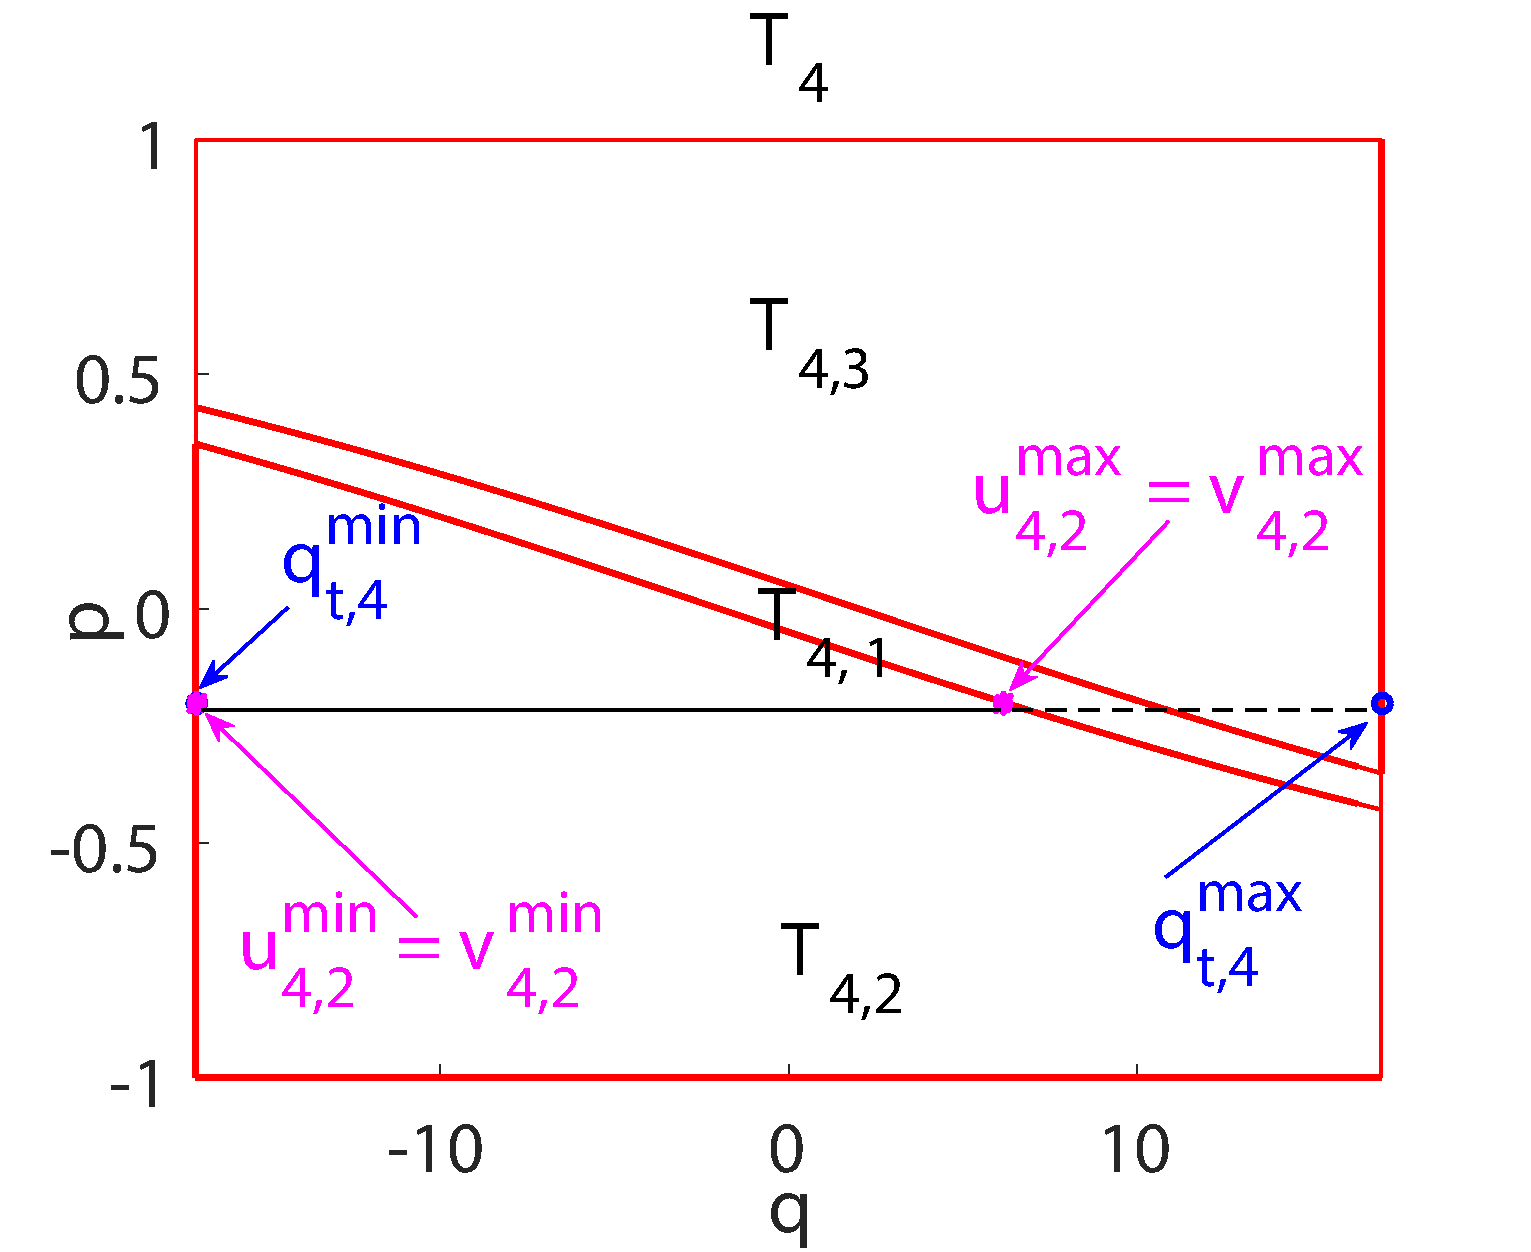
\includegraphics[width=\textwidth]{T4_2}
   \caption{\footnotesize{\textbf{Target PS of line $4$.}
  The intersection points between the line $\variabile{p} = -0.2$ and $\partial$\set{T}{$4$,}{$2$} are $(\variabile{u}_{4,2}^{\textrm{min}}, \variabile{p})$ and
  $(\variabile{u}_{4,2}^{\textrm{max}}, \variabile{p})$. $\variabile{v}_{4,2}^{\textrm{min}}= \max \{\pos{t,}{$4$}^{\textrm{min}}, \variabile{u}_{4,2}^{\textrm{min}}\}$ and
  $\variabile{v}_{4,2}^{\textrm{max}}= \min \{\pos{t,}{$4$}^{\textrm{max}}, \variabile{u}_{4,2}^{\textrm{max}}\}$.\\}}
   \label{fig:T42}
 \end{minipage}\hfill
 \begin{minipage}[t]{.48\textwidth}
   \centering
   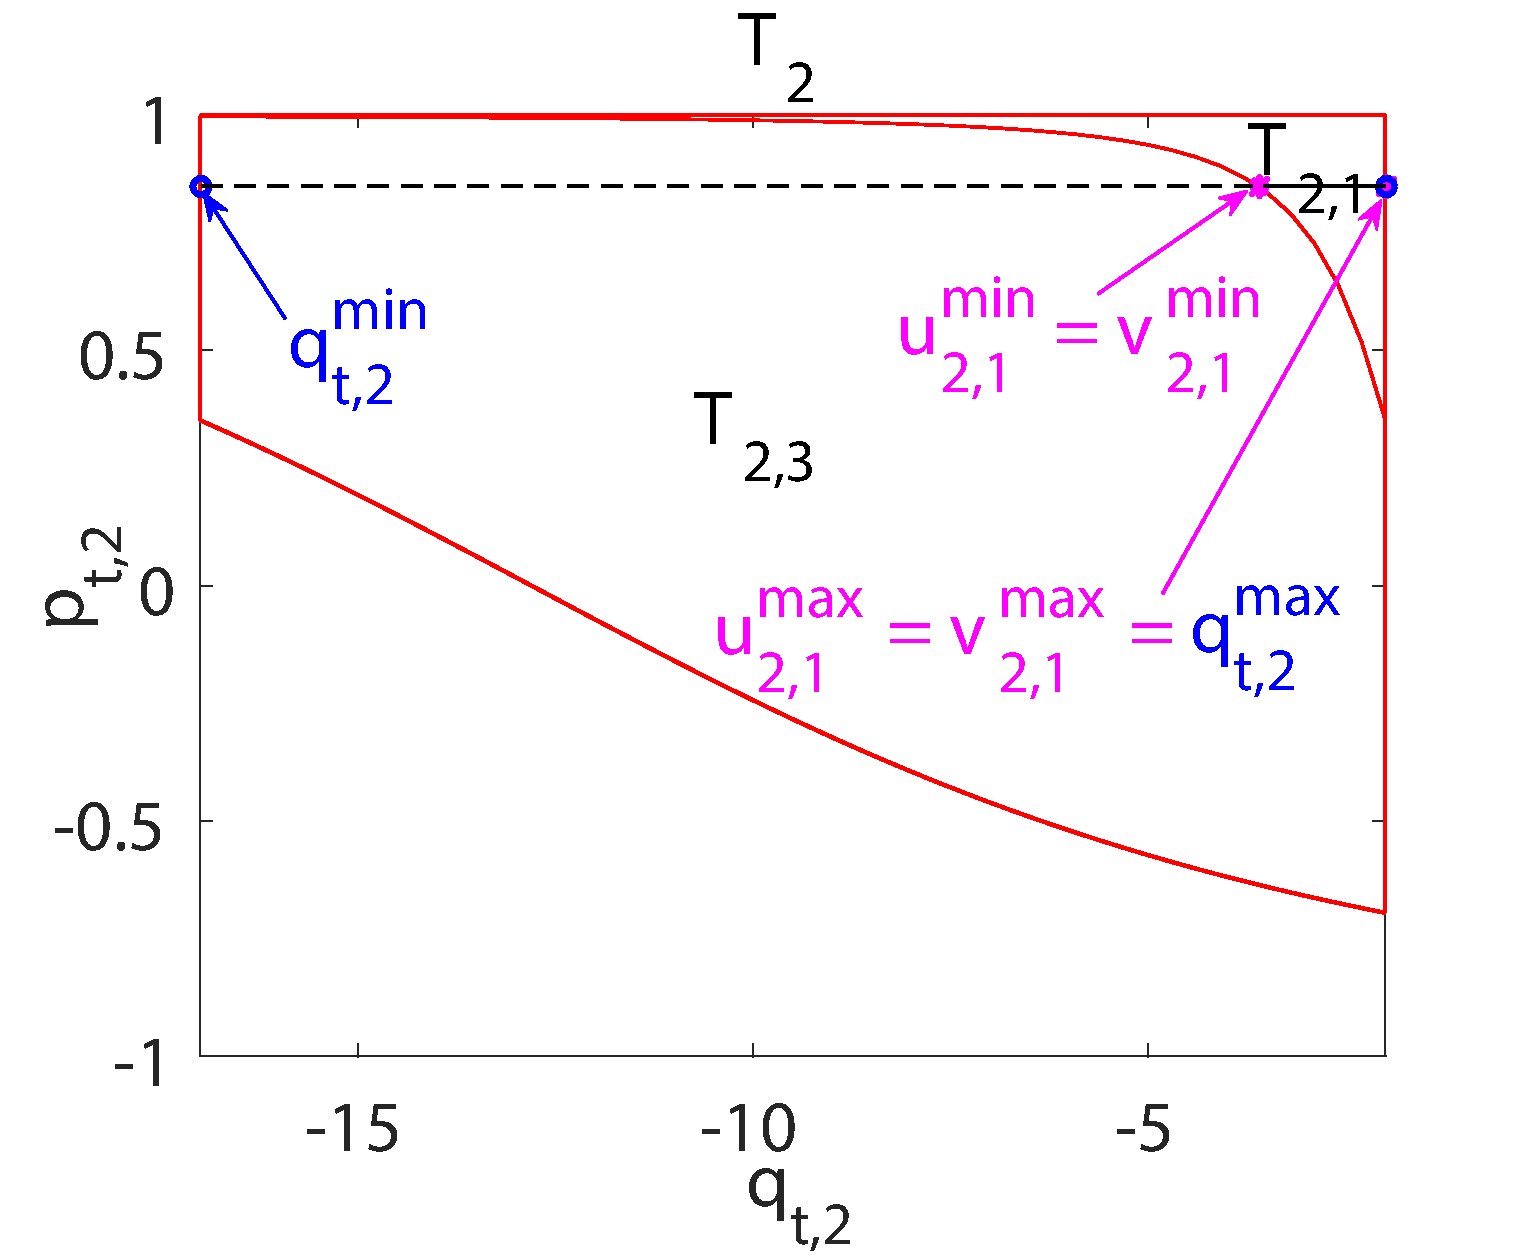
\includegraphics[width=\textwidth]{T2_1}
   \caption{\footnotesize{\textbf{Target PS of line $2$.} The coordinates of the intersection points between the line $\dir{t,}{$2$} = 0.82$ and $\partial$\set{T}{$2$,}{$1$} are
  $(\variabile{u}_{2,1}^{\textrm{min}}, \dir{t,}{$2$})$ and $(\variabile{u}_{2,1}^{\textrm{max}}, \dir{t,}{$2$})$.
  $\variabile{v}_{2,1}^{\textrm{min}}= \max \{\pos{t,}{$2$}^{\textrm{min}}, \variabile{u}_{2,1}^{\textrm{min}}\}$ and
  $\variabile{v}_{2,1}^{\textrm{max}}= \min \{\pos{t,}{$2$}^{\textrm{max}}, \variabile{u}_{2,1}^{\textrm{max}}\}$.}}
    \label{fig:T21}
 \end{minipage}\hfill
 \begin{minipage}[t]{.48\textwidth}
  \centering
   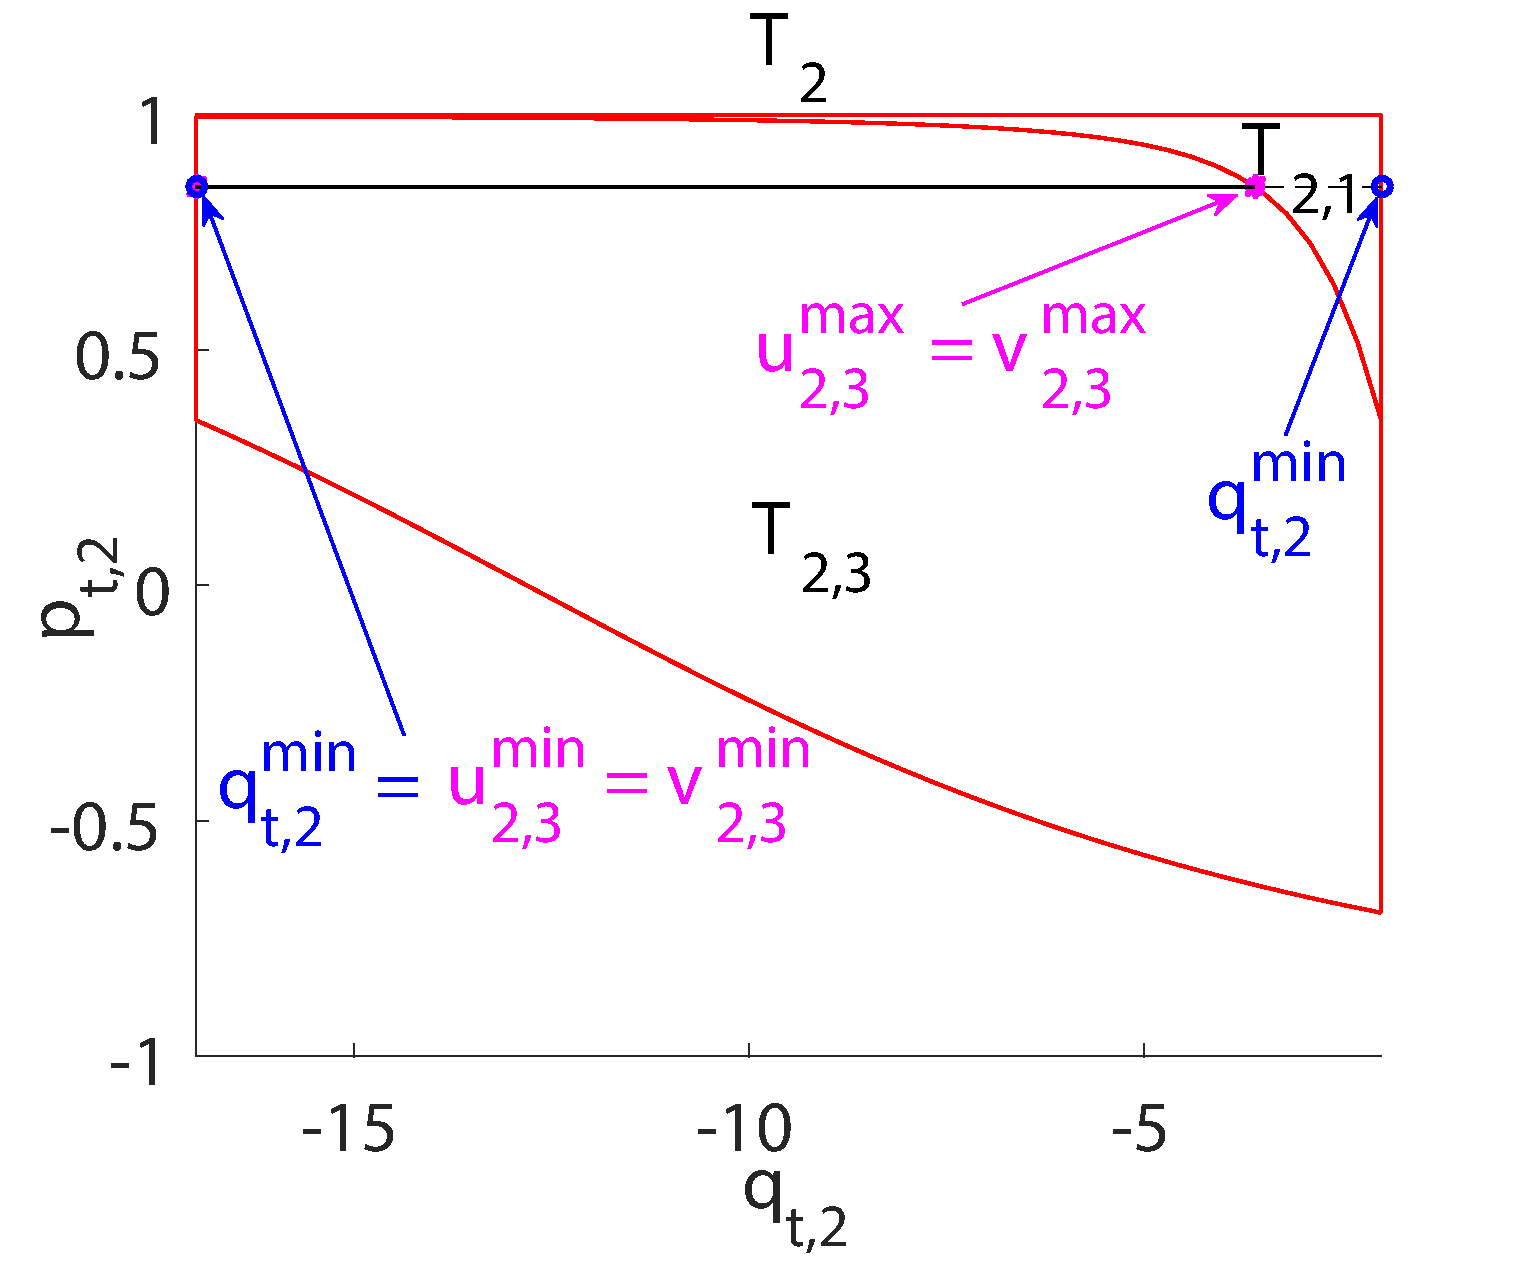
\includegraphics[width=\textwidth]{T2_2}
\caption{\footnotesize{\textbf{Target PS of line $2$.}
  The coordinates of the intersection points between the line $\dir{t,}{$2$}=0.82$ and $\partial$\set{T}{$2$,}{$3$} are
  $(\variabile{u}_{2,3}^{\textrm{min}}, \dir{t,}{$2$})$ and $(\variabile{u}_{2,3}^{\textrm{max}}, \dir{t,}{$2$})$.
  $\variabile{v}_{2,3 }^{\textrm{min}} = \max\{\pos{t,}{$2$}^{\textrm{min}}, \variabile{u}_{2,3}^{\textrm{min}}\}$ and
   $\variabile{v}_{2,3 }^{\textrm{max}} = \min\{\pos{t,}{$3$}^{\textrm{max}}, \variabile{u}_{2,3}^{\textrm{max}}\}$.}}
 \label{fig:T22}
 \end{minipage}\hfill
%\hspace{3cm}
 \end{figure}
 \begin{figure}
\begin{minipage}[t]{.48\textwidth}
   \centering
   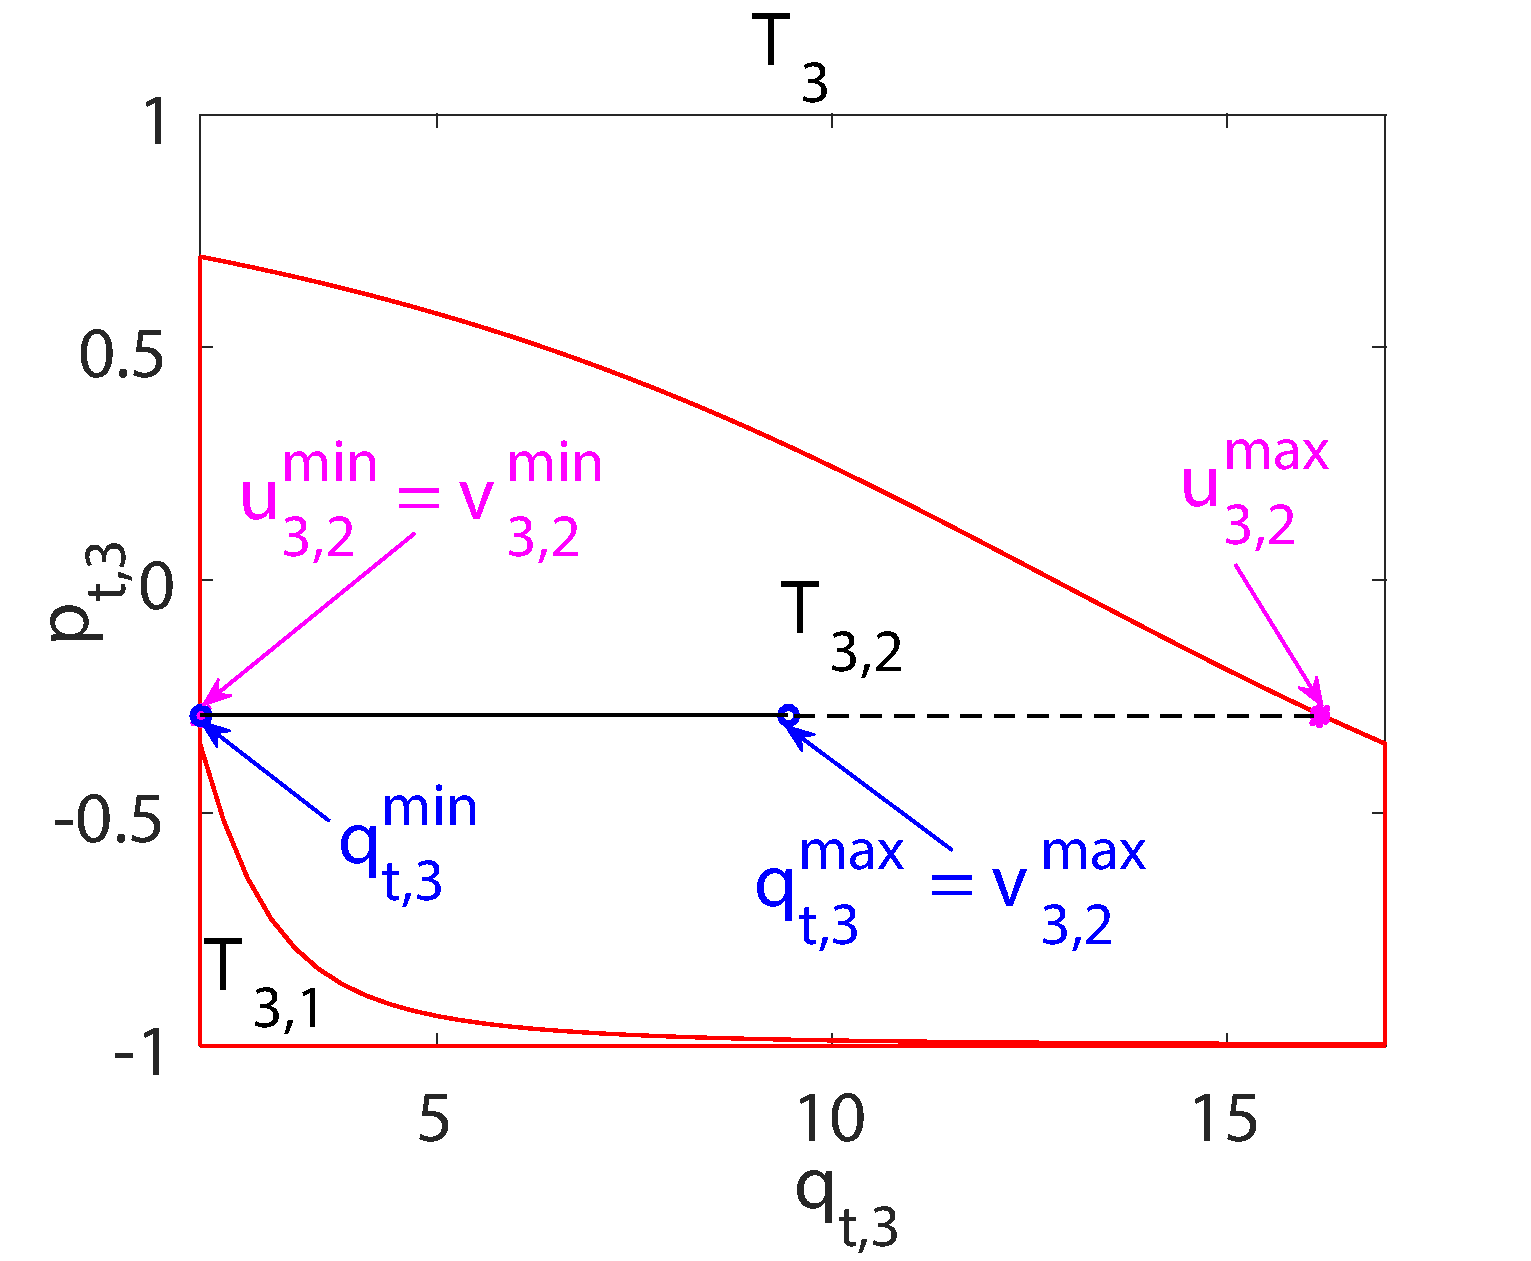
\includegraphics[width=\textwidth]{T3_1}
   \caption{\footnotesize{\textbf{Target PS of line $3$.}
  The position coordinates of the intersection points between  the line $ \dir{t,}{$3$} = -0.29$ and
  $\partial$\set{T}{$3$,}{$2$} are $\variabile{u}_{3,2}^{\textrm{min}}$ and $\variabile{u}_{3,2}^{\textrm{max}}$.
   $\variabile{v}_{3,2 }^{\textrm{min}} = \max\{\pos{t,}{$3$}^{\textrm{min}}, \variabile{u}_{3,2}^{\textrm{min}}\}$ and
   $\variabile{v}_{3,2 }^{\textrm{max}} = \min\{\pos{t,}{$3$}^{\textrm{max}}, \variabile{u}_{3,2}^{\textrm{max}}\}$.\\}}
   \label{fig:T31}
 \end{minipage}\hfill
 \begin{minipage}[t]{.48\textwidth}
  \centering
   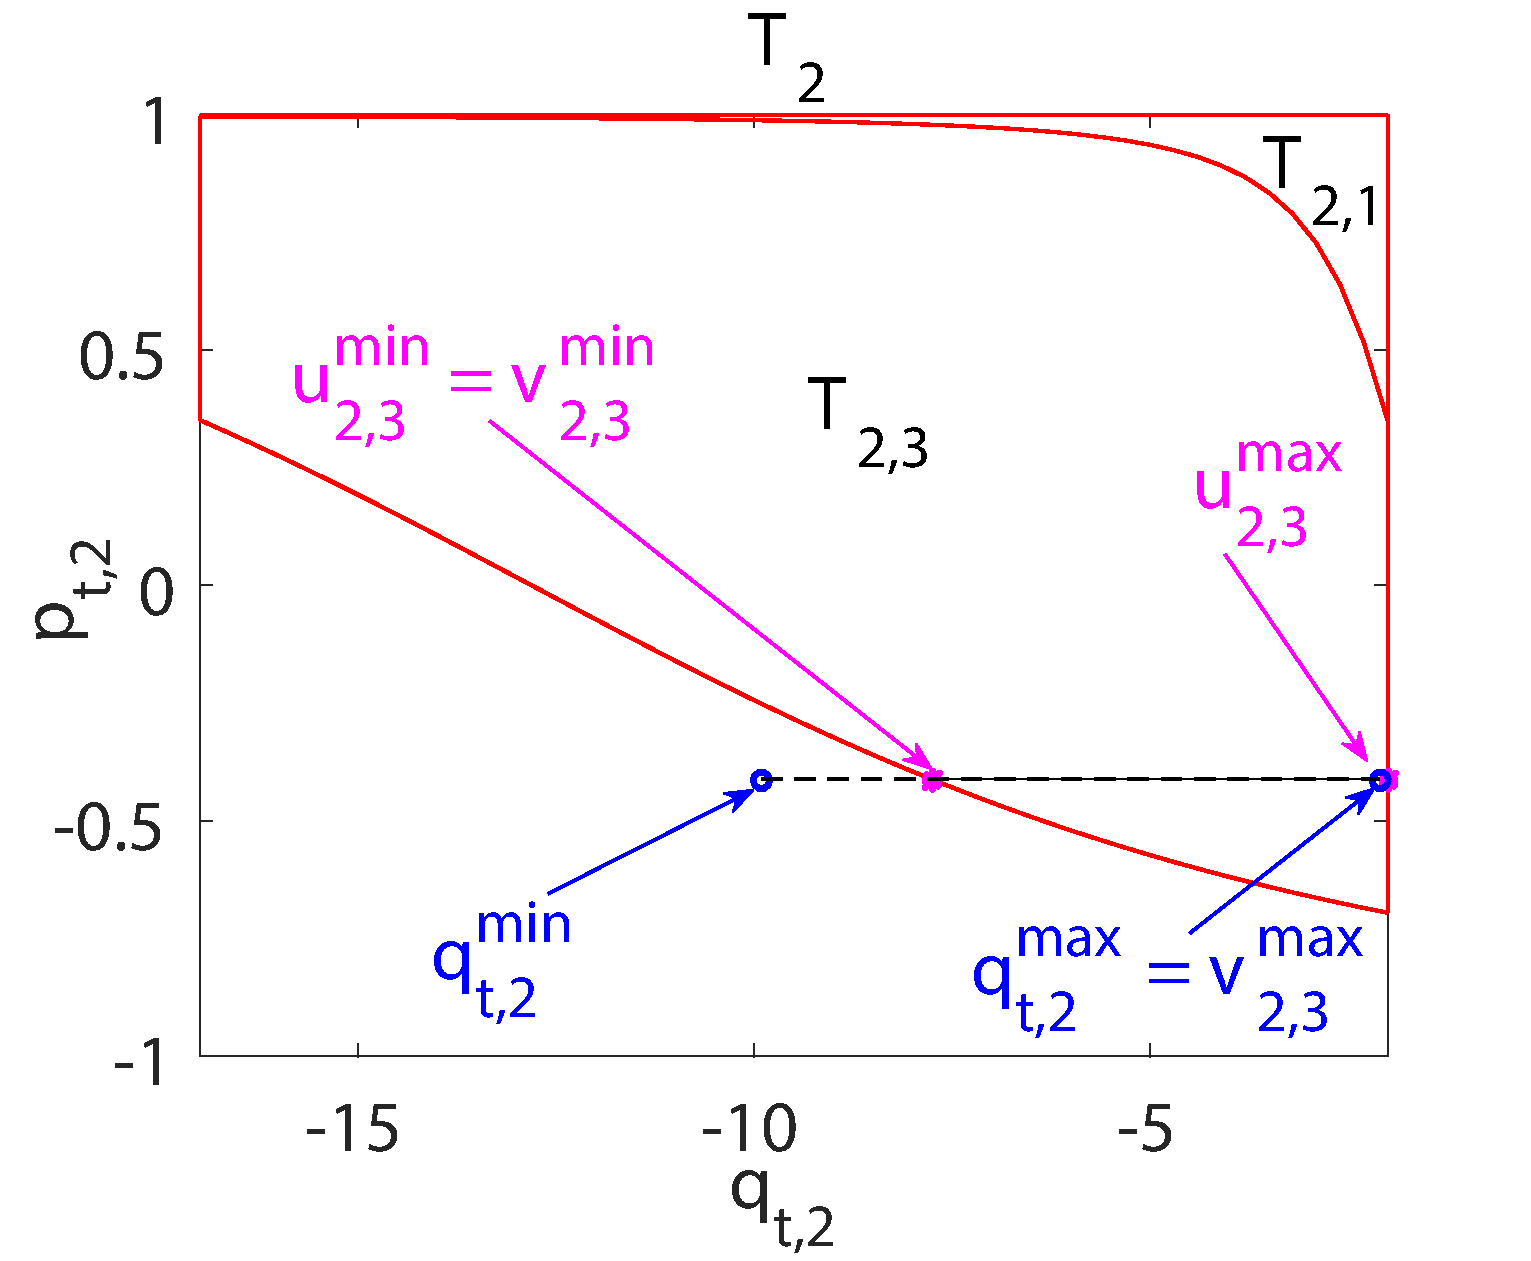
\includegraphics[width=\textwidth]{T2_3}
\caption{\footnotesize{\textbf{Target PS of line $2$.}
 The intersection points between the line $\dir{t}{} = \dir{t,}{$2$}$ and $\partial$\set{T}{$2$,}{$3$} are
 $(\variabile{u}_{2,3}^{\textrm{min}}, \dir{t,}{$2$})$ and $(\variabile{u}_{2,3}^{\textrm{max}}, \dir{t,}{$2$})$.
 $\variabile{v}_{2,3 }^{\textrm{min}} = \max\{\pos{t,}{$2$}^{\textrm{min}}, \variabile{u}_{2,3}^{\textrm{min}}\}$ and
 $\variabile{v}_{2,3 }^{\textrm{max}} = \min\{\pos{t,}{$2$}^{\textrm{max}}, \variabile{u}_{2,3}^{\textrm{max}}\}$.\\}}
    \label{fig:T23}
 \end{minipage}\hfill
  \begin{minipage}[t]{.48\textwidth}
   \centering
   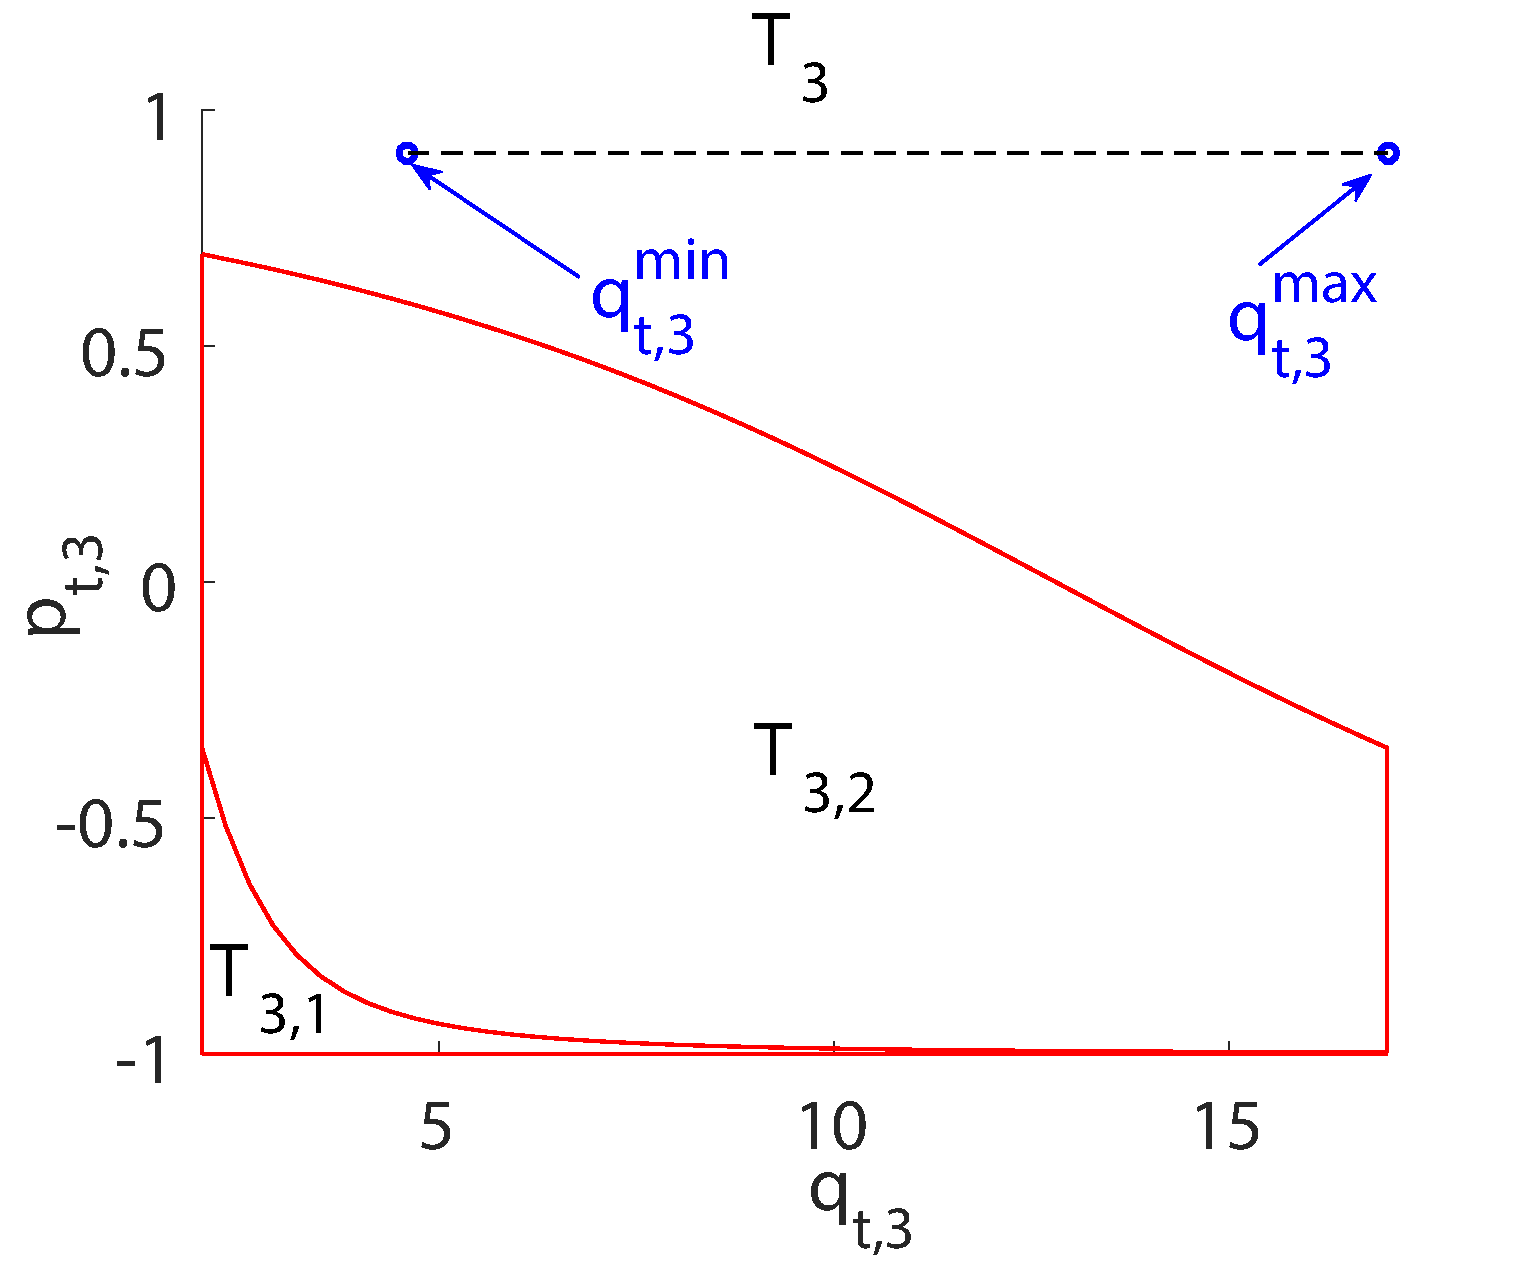
\includegraphics[width=\textwidth]{T3_2}
   \caption{\footnotesize{\textbf{Target PS of line $3$.} 
  There are no intersection points of the line $\dir{$3$,}{$2$}=0.91$
 with the boundaries $\partial$\set{T}{$3$,}{$2$} and $\partial$\set{T}{$3$,}{$1$}.
  The rays with coordinates inside the dotted segment hit again line $4$ after some reflections and, therefore, are not emitted by the source.}}
    \label{fig:T32}
 \end{minipage}\hfill
 \begin{minipage}[t]{.48\textwidth}
   \centering
   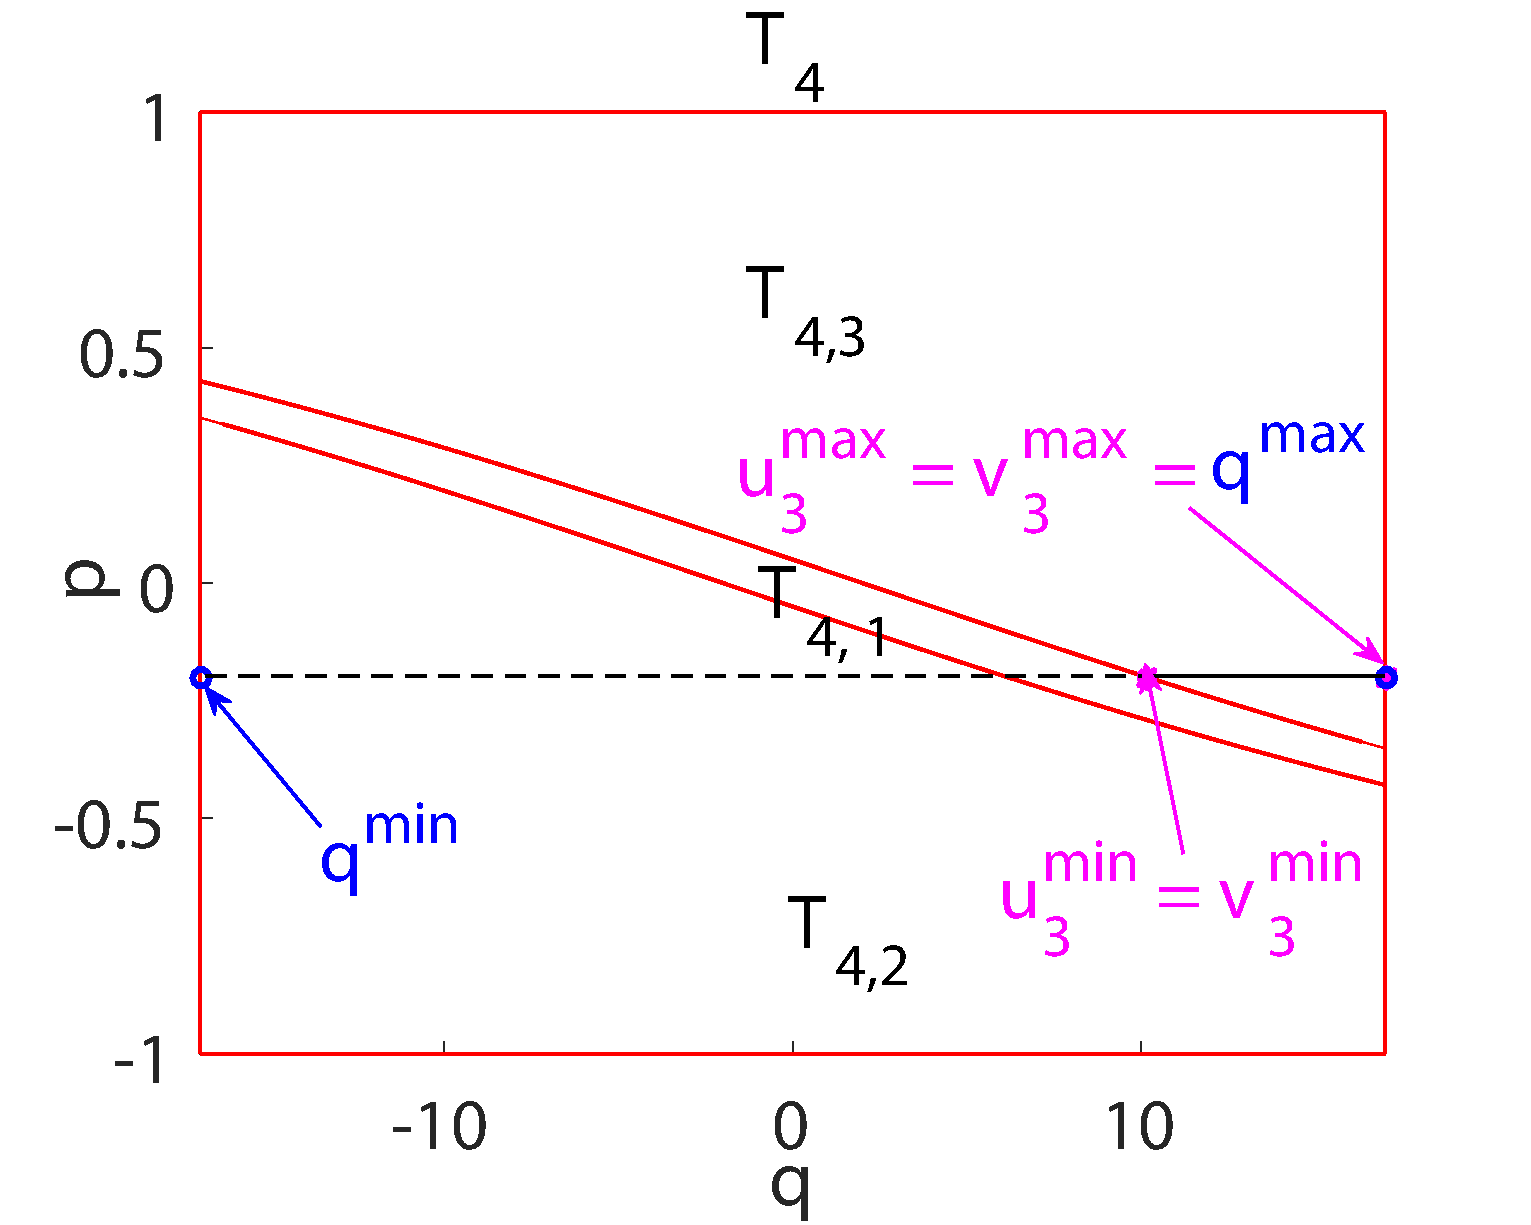
\includegraphics[width=\textwidth]{T4_3}
   \caption{\footnotesize{\textbf{Target PS of line $4$.} $\pos{t,}{$4$}^{\textrm{min}} = -\variabile{b}$ and $\pos{t,}{$4$}^{\textrm{max}}= \variabile{b}$.
  The intersection points between the line $\variabile{p} = -0.2$ and $\partial$\set{T}{$4$,}{$3$} are $(\variabile{u}_{4,3}^{\textrm{min}}, \variabile{p})$ and $(\variabile{u}_{4,3}^{\textrm{max}}, \variabile{p}).$ $\variabile{v}_{4,3}^{\textrm{min}} = \max\{\pos{t,}{$4$}^{\textrm{min}}, \variabile{u}_{4,3}^{\textrm{min}}\}$
  and $\variabile{v}_{4,3}^{\textrm{max}} = \min\{\pos{t,}{$4$}^{\textrm{max}}, \variabile{u}_{4,3}^{\textrm{max}}\}$.}}
   \label{fig:T43}
\end{minipage}\hfill
%\hspace{3cm}
\end{figure}
\begin{algorithm}
\caption{Recursive procedure for the intensity calculation}\label{alg}
Initialize {$\lineaj=4,$  $\pos{t,}{$4$}^\textrm{\,min} = \variabile{q}^{\textrm{min}} = -\variabile{b},$ 
 $\pos{t,}{$4$}^ \textrm{\,max}= \variabile{q}^{\textrm{max}}=\variabile{b},$ $\dir{t,}{$4$} = \dir{}{} =  \mbox{const},$  $\Pi = (4)$. }
\begin{algorithmic}[1]
\Procedure {Intensity computation}{$\lineaj$, $\pos{t,}{\lineaj}^\textrm{\,min},$  $\pos{t,}{\lineaj}^ \textrm{\,max},$ $\dir{t,}{\lineaj},$  $\Pi$}
\For{$ \lineai =  1, 2, 3 $}
   \If{$\lineai\neq\lineaj$}
   \State Compute the intersection points 
    $(\variabile{u}_{\lineaj, \lineai}^\textrm{\,min}, \dir{t,}{\lineaj})$ and $(\variabile{u}_{\lineaj, \lineai}^\textrm{\,max}, \dir{t,}{\lineaj})$
   %between $\dir{t,}{\lineaj}$ and $\partial$\set{T}{\lineaj,}{\lineai}
 \State $\Pi=(\lineai, \Pi)$
           \State Compute 
%          \begin{equation*}
     $      [\variabile{v}_{\lineaj, \lineai}^\textrm{\,min}, \variabile{v}_{\lineaj, \lineai}^\textrm{\,max}] = [\variabile{u}_{\lineaj, \lineai}^\textrm{\,min}, \variabile{u}_{\lineaj, \lineai}^\textrm{\,max}]\cap
           [\pos{t,}{\lineaj}^\textrm{\,min}, \pos{t,}{\lineaj}^\textrm{\,min}] $
  %        \end{equation*}
       \If{($\lineai\neq 1)$  \& $ (\lineai\neq 4)$}
           \State Trace back from \set{T}{\lineaj}{} to \set{T}{\lineai}{}
           \begin{equation*}
           \begin{aligned}
           (\pos{t,}{\lineai}^{\,1}, \dir{t,}{\lineai})& =\inversemap{R}{\lineai}{}\circ \inversemap{P}{\lineai,}{\lineaj}(\variabile{v}_{\lineaj,\lineai}^\textrm{\,min}, \dir{t,}{\lineaj})  \\
           (\pos{t,}{\lineai}^{\,2}, \dir{t,}{\lineai}) & =\inversemap{R}{\lineai}{}\circ \inversemap{P}{\lineai,}{\lineaj}(\variabile{v}_{\lineaj,\lineai}^\textrm{\,max}, \dir{t,}{\lineaj})
           \end{aligned}
           \end{equation*}
           \State Determine \begin{equation*}
\pos{t,}{\lineai}^\textrm{\,min}= \min\{\pos{t,}{\lineai}^{\,1}, \pos{t,}{\lineai}^{\,2}\} \mbox{ and }
\pos{t,}{\lineai}^\textrm{\,max}= \max\{\pos{t,}{\lineai}^{\,1}, \pos{t,}{\lineai}^{\,2}\}
\end{equation*}
          \State\Return{\Call{Intensity computation}{$\lineai$, $\pos{t,}{\lineai}^\textrm{\,min},$  $\pos{t,}{\lineai}^ \textrm{\,max},$ $\dir{t,}{\lineai},$  $\Pi$}}
       \Else 
\If{\lineai=1}
              \If{$\lineaj\neq4$}
                 \State Trace back from \set{T}{\lineaj}{} to \set{S}{$1$}{}, next apply the forward map $\mapnumb{M}_{1,4}(\Pi)$
\begin{equation*}
\begin{aligned}
(\pos{s,}{$1$}^{\,1}, \dir{s,}{$1$})& = \inversemap{P}{1,}{\lineaj}(\variabile{v}_{\lineaj,1 }^\textrm{\,min}, \dir{t,}{\lineaj})  \\
(\pos{s,}{$1$}^{\,2}, \dir{s,}{$1$}) & =\inversemap{P}{1,}{\lineaj}(\variabile{v}_{\lineaj, 1}^\textrm{\,max}, \dir{t,}{\lineaj})\\
(\pos{}{}^{1}(\Pi, \dir{}{}), \dir{}{})&= \mapnumb{M}_{1,4}(\Pi)(\pos{s,}{$1$}^{\,1}, \dir{s,}{$1$})\\
(\pos{}{}^{2}(\Pi, \dir{}{}), \dir{}{})&= \mapnumb{M}_{1,4}(\Pi)(\pos{s,}{$1$}^{\,2}, \dir{s,}{$1$})
\end{aligned}
\end{equation*}
%\State Apply 
%\begin{equation*}
%\begin{aligned}
% (\pos{}{}^{1}(\Pi, \dir{}{}), \dir{}{})&= \mapnumb{M}_{1,4}(\Pi)(\pos{s,}{1}^{\,1}, \dir{s,}{1})\\
% (\pos{}{}^{2}(\Pi, \dir{}{}), \dir{}{})&= \mapnumb{M}_{1,4}(\Pi)(\pos{s,}{1}^{\,2}, \dir{s,}{1})
%\end{aligned}
%\end{equation*}
\State Calculate
\begin{equation*}
\begin{aligned}
\pos{}{}^\textrm{\,min}(\Pi,\dir{}{})&= \min\{\pos{}{}^{\,1}, \pos{}{}^{\,2}\} \\ 
\pos{}{}^\textrm{\,max}(\Pi,\dir{}{})&= \max\{\pos{}{}^{\,1}, \pos{}{}^{\,2}\}
\end{aligned}
\end{equation*}
\State where $\pos{}{}^{\,1} := \pos{}{}^{\,1}(\Pi, \dir{}{})$ and $\pos{}{}^{\,2} := \pos{}{}^{\,2}(\Pi, \dir{}{})$.
                 \State\Return{$I(\variabile{p})= I(\variabile{p})+\variabile{q}^\textrm{\,max}(\Pi, \dir{}{})-\variabile{q}^\textrm{\,min}(\Pi, \dir{}{})$}
                 \Else
                 \begin{equation*}
                    %   \begin{aligned}
                       \variabile{q}^\textrm{\,min}(\Pi, \dir{}{}) = \variabile{v}_{4, \lineaj}^\textrm{\,min}, 
                       \variabile{q}^\textrm{\,max}(\Pi, \dir{}{}) = \variabile{v}_{4, \lineaj}^\textrm{\,max}
                    %   \end{aligned}
                       \end{equation*}
                  \State\Return{$I(\variabile{p})= I(\variabile{p})+\variabile{q}^\textrm{\,max}(\Pi, \dir{}{})-\variabile{q}^\textrm{\,min}(\Pi, \dir{}{}).$}
              \EndIf    
\Else \pagebreak
\State \Return $I(\variabile{p})$
\EndIf
        \EndIf
     \EndIf
\EndFor
\EndProcedure
\end{algorithmic}
\end{algorithm}
 \\ \indent In the next section we provide the numerical results for the two-faceted cup. 
\section{Numerical results for the two-faceted cup}
To demonstrate the accuracy of the method, a comparison with MC and QMC ray tracing is provided.
The MC and QMC intensities are computed as explained in Chapter \ref{chap:raytracing}. 
We consider here the same partitioning $P:-1 = \variabile{p}^0 < \cdots< \variabile{p}^\textrm{Nb} = 1$ of the interval $[-1,1]$ used for all the simulations presented in the previous chapters. 
The profile of the QMC intensity is obtained tracing $10^7$ rays and taking $\textrm{Nb} = 100$.% is depicted in Figure \ref{fig:intensity_cup} with a blue line.\\
\\ \indent  The PS intensity is obtained from (\ref{eta2}) where the rays on the boundaries are obtained applying backward ray mapping. We observe that the method is suitable for detecting all the possible paths $\Pi$ that a ray can follow during the propagation through the system. According to the results obtained with PS ray tracing, $5$ different paths are found for the two-faceted cup. Given a path $\Pi$, the coordinates $(\variabile{q}^\textrm{min}(\Pi, \variabile{p}^ \variabile{h}), \variabile{p}^ \variabile{h})$ and $(\variabile{q}^\textrm{\,max}(\Pi, \variabile{p}^ \variabile{h}), \variabile{p}^\variabile{h})$ of the corresponding rays located on $\partial \mbox{\set{R}{}{}}(\Pi)$ are determined for every $\variabile{p} = (\variabile{p}^\variabile{h})_{\variabile{h}=0, \cdots, \textrm{Nb}}$ where the values $\variabile{p}^\variabile{h}$ are chosen from the partitioning $P$ used for QMC ray tracing. These rays are depicted in Figure \ref{fig:final_T}, where all the rays that follow the same path are shown with the same color. For the two-faceted cup, given a direction $\variabile{p}^\variabile{h}$ and a path $\Pi$, only two rays are located on the boundary $\partial$\set{R}{}{}$(\Pi)$ of the corresponding region along that direction. As a consequence, at most $2\,\npath\,\textrm{Nb}$ rays need to be traced from the target to the source, where $\npath =5$ is the number of paths.
The averaged normalized PS intensity is given by Equation (\ref{eq:normalized_PS_intensity})
%\begin{equation}\label{eq:intensity}
% \hat{I}_{\textrm{PS}}(\variabile{p}^{\variabile{h}+1/2}) = \frac{\int_{\variabile{p}^\variabile{h}}^{\variabile{p}^{\variabile{h}+1}}{\lineai}_{PS}(\variabile{p})\textrm{d}\variabile{p}}{\int_{-1}^{1}{\lineai}_{PS}(\variabile{p})\textrm{d}\variabile{p}}\,,
% \end{equation}
%for $\variabile{h} = 0,1, \cdots, \textrm{Nb}-1,$
 where the integrals are calculated using the trapezoidal rule.
\begin{figure}[t]
  \begin{center}
  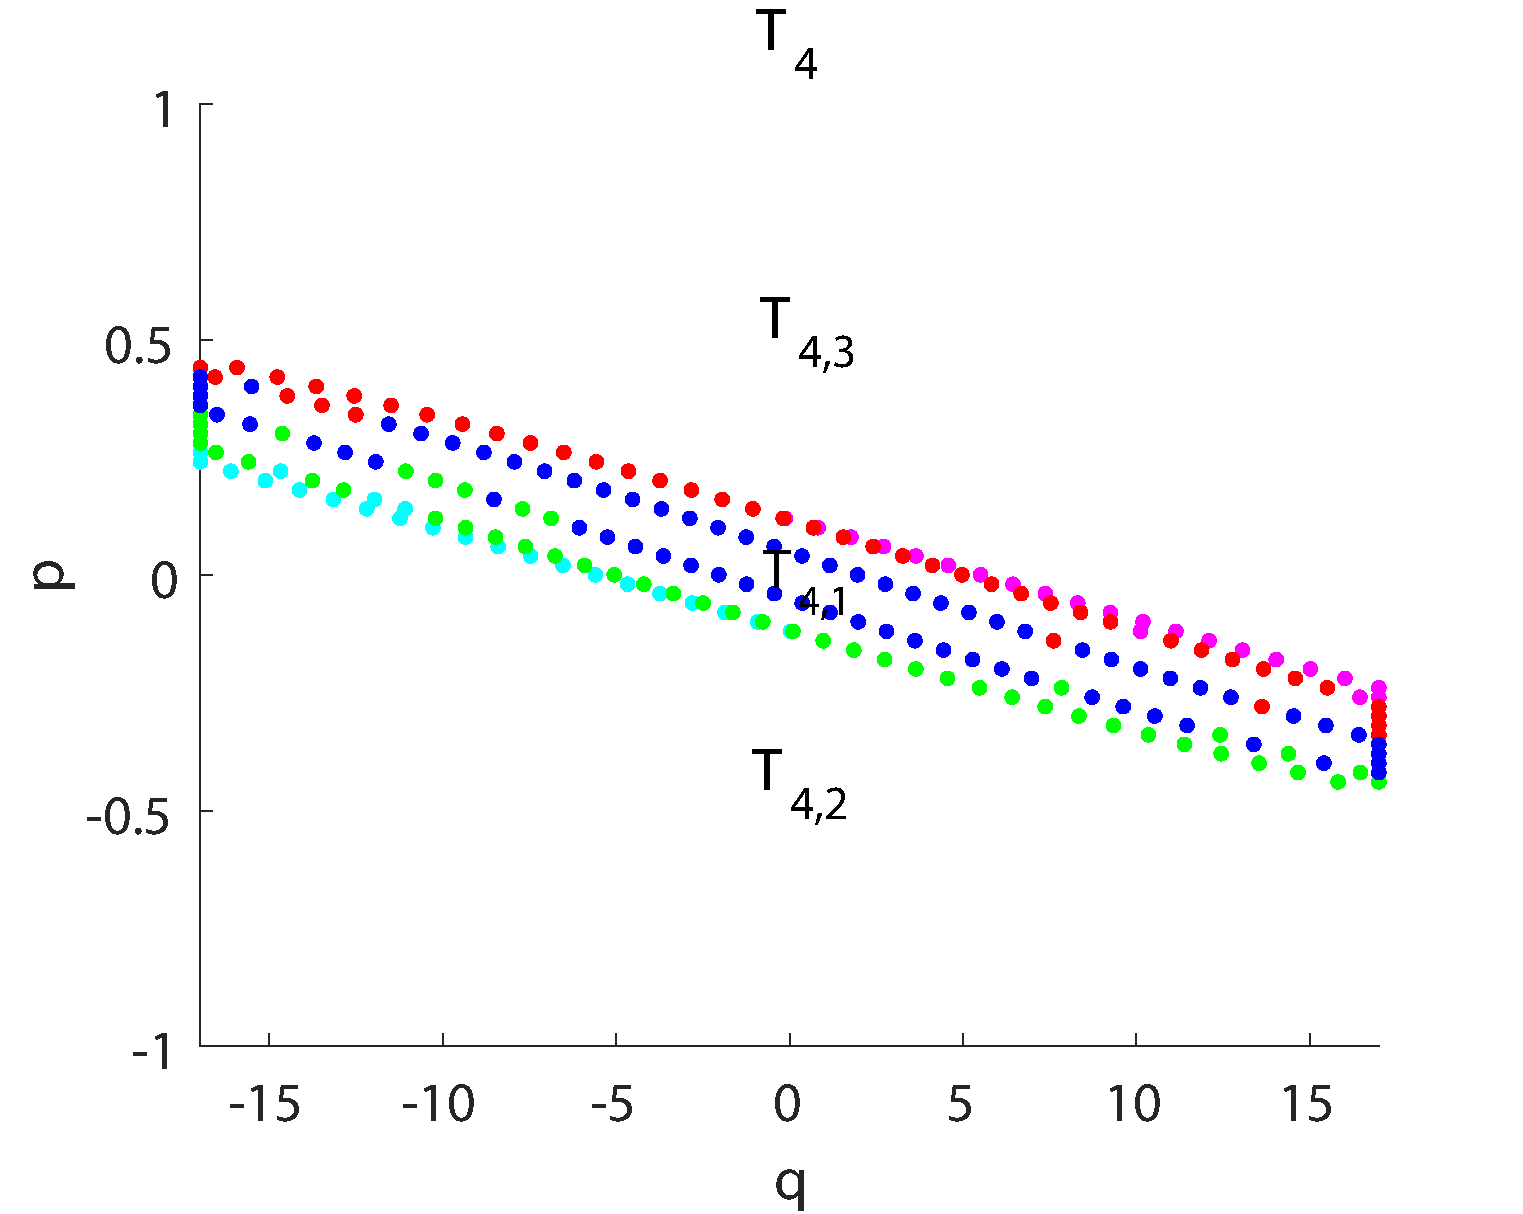
\includegraphics[scale=.4]{final_T}
  \end{center}
  \caption{\textbf{Target phase space of the two-faceted cup divided into $100$ bins.}
  Five different paths are found. The rays with coordinates $(\variabile{q}^\textrm{\,min}, \variabile{p})$ and $(\variabile{q}^\textrm{\,max}, \variabile{p})$ in \set{T}{$4$}{} that are located at the boundaries $\partial \mbox{\set{R}{}{}}(\Pi)$ are depicted with dots, the color of the dots depends on the path $\Pi$ followed by the rays.
  Using the ray mapping method, only these rays need to be traced from $\point{S}$ to $\point{T}$ for the intensity computation.}
  \label{fig:final_T}
\end{figure} 
%The profile of the PS intensity is depicted in in Figure \ref{fig:intensity_cup} with the dotted green line.
The approximated intensities $\hat{I}_{\textrm{A}} (\textrm{A} = \textrm{MC}, \textrm{QMC},  \textrm{PS})$ are compared to the reference intensity $\hat{I}_\textrm{ref}$ which in this case in the exact intensity ($\hat{I}_{\textrm{ref}}=\hat{I}_{\textrm{exact}}$). The results in Figure \ref{fig:intensity_cup} show that our method computes the intensity correctly. 
 \\ \indent
To compare the speed of convergence of the three methods, we consider the error between the approximate intensities $\hat{I}_{\textrm{A}}$ ($\textrm{A} = \textrm{MC}, \textrm{QMC}, \textrm{PS}$) and the exact intensity $\hat{I}_{\mbox{exact}} = \hat{I}_{\mbox{ref}}$.
The three errors as a function of the CPU-time are depicted in a logarithmic scale in Figure $\ref{fig:error_cup}$. Numerical results show that MC ray tracing converges proportionally to the inverse of the square root of the number of rays traced, QMC error is proportional to the inverse of the number of rays, backward ray mapping is able to compute the output intensity of the two-faceted cup exactly. Also, it is much faster than MC ray tracing when an error smaller than $10^{-4}$ is required and it is faster than QMC ray tracing if an error smaller than around $10^{-5}$ is desired.
\begin{figure}[t]
  \begin{center}
  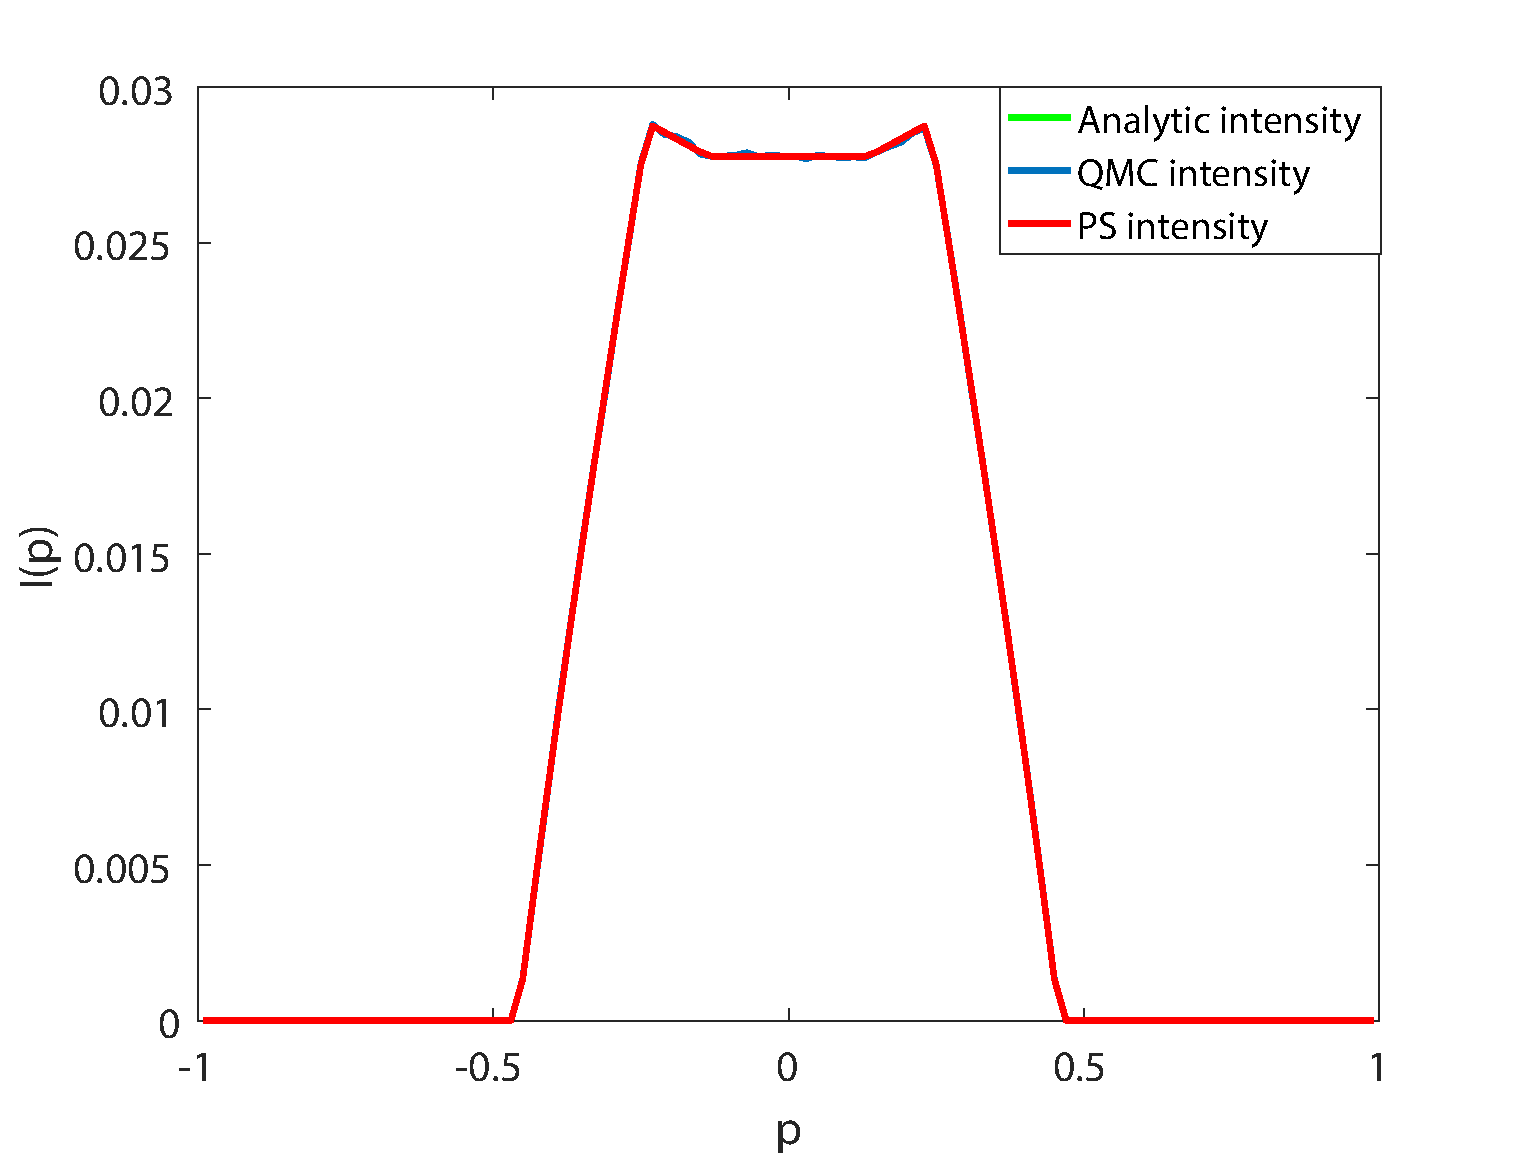
\includegraphics[scale=.4]{intensity_cup_raymapping}
  \end{center}
  \caption{\textbf{Intensities for the two-faceted cup.} The intensities found with three different approaches are shown.}
  \label{fig:intensity_cup}
\end{figure}
\begin{figure}[h]
  \begin{center}
  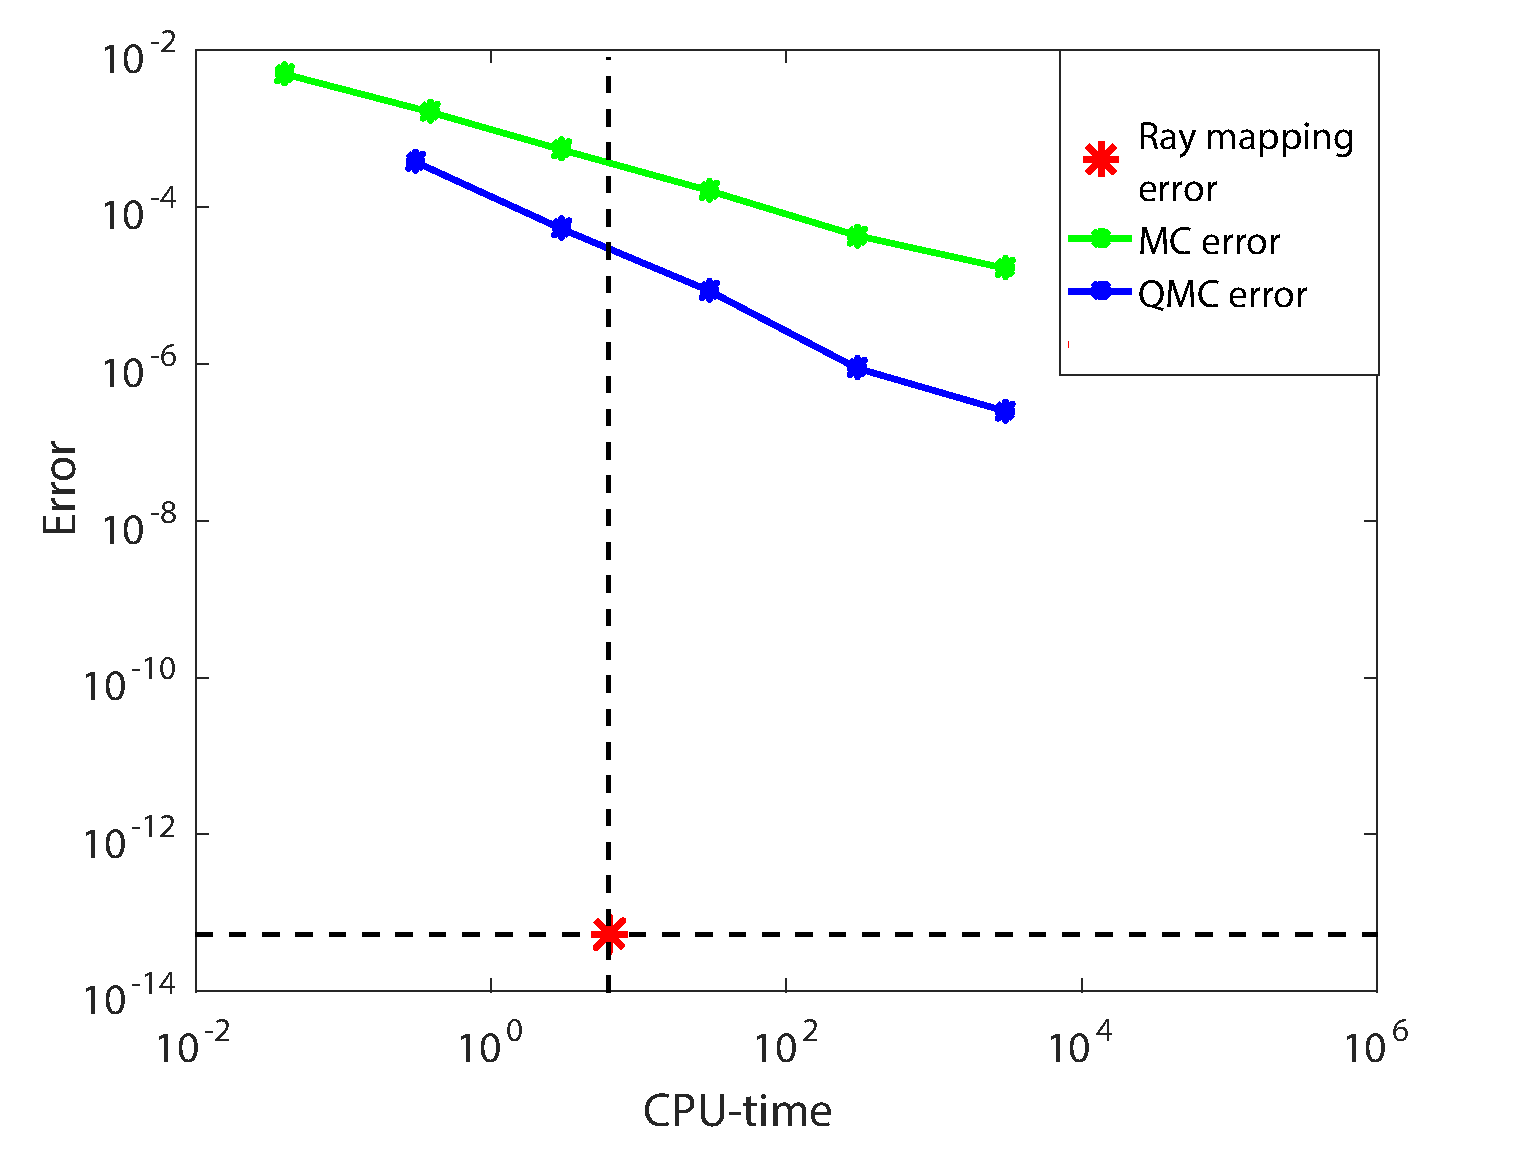
\includegraphics[scale=.4]{error_cup_raymapping}
  \end{center}
  \caption{\textbf{Errors for the two-faceted cup.} The errors are depicted as a function of the CPU time (in seconds).}
  \label{fig:error_cup}
\end{figure}
\section{Extension of the method for the multi-faceted cup}
\label{sec:Generalization}
The method can be generalized to more complicated optical systems.
In particular, it can be used for all systems formed by straight line segments.
The goal of this section is to show the generalization of the method to the multi-faced cup which is a system with many left and right segments as reflectors.
The design of this system is explained below. \\ \indent
A multi-faceted cup is an optical system formed by a source, a target and $\nline-2$ reflectors, where $\nline$ is the number of optical line segments that form the system.
Defining a Cartesian coordinate system $(\variabile{x}, \variabile{z})$, the multi-faceted cup is symmetric with respect to the optical axis (\variabile{z}-axis). An example of this system is depicted in Figure \ref{fig:multifacetedcup} where all the lines are labeled with numbers.
The source $\point{S}= [-\variabile{a}, \variabile{a}]$ (line $1$) and the target $\point{T}= [-\variabile{b}, \variabile{b}]$ (line $22$) are two segments both perpendicular to the optical axis, with $\variabile{a}=2$ and $\variabile{b}=17$.
$\point{S}$ is located at the height $\variabile{z}=0$ while $\point{T}$ has a height $\variabile{z}=40$.
Both sides of the system are divided into $10$ segments which connect $\point{S}$ with $\point{T}$.
The ten adjacent segments at the left of the system (lines $2, \cdots, 11$) connect the left extreme of the source with the left extreme of the target.
Similarly, ten adjacent segments at the right of the system (lines $12, \cdots, 21$) connect the right extreme of the source with the right extreme of the target.
These segments are designed as follows. The intervals $[-\variabile{b}, -\variabile{a}]$ and $[\variabile{a}, \variabile{b}]$ are divided into ten sub-intervals of the same length $(\variabile{b}-\variabile{a})/10$.
The \variabile{x}-coordinates of the end points of the line segments $12, \cdots, 21$ are equal to the \variabile{x}-coordinates of the sub-intervals of $[\variabile{a},\variabile{b}]$, while the \variabile{x}-coordinates of the end points of the line segments $2, \cdots, 11$ are equal to the \variabile{x}-coordinates of the sub-intervals of $[-\variabile{a},-\variabile{b}]$.
The \variabile{z}-coordinates of every end point of the line segments $2, \cdots, 21$  are given substituting their $\variabile{x}$-coordinates into the equation of the parabola whose symmetry axis is equal to the \variabile{z}-axis and that passes through the
points $(-17,40)$ and $(17,40)$. The $20$-faceted cup is now well defined and can be seen as an approximation of a parabolic reflector.
\begin{figure}[h]
\centering
\label{fig:multifacetedcup}
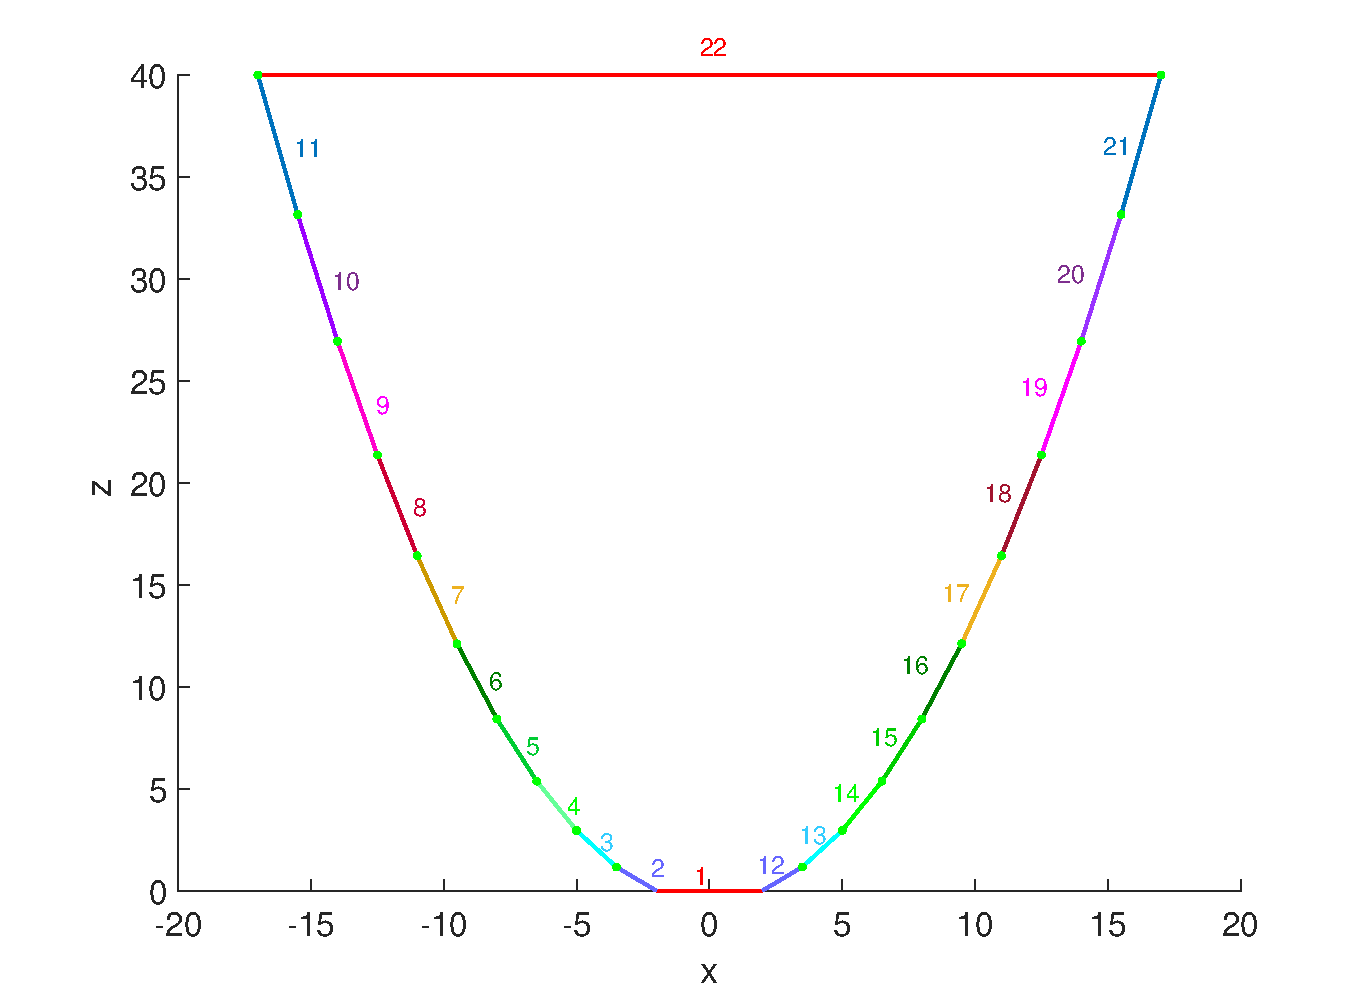
\includegraphics[scale=.4]{multifacetedcup1}
\caption{\textbf{The $20$-faceted cup.} The system is formed by $22$ different line segments: the source $\point{S}$, the target
$\point{T}$, ten left reflectors and ten right reflectors.
 $\point{S}=[-2,2]$ is located at $\variabile{z}=0$. $\point{T} = [-17,17]$ is parallel to the source and it is located at a height $\variabile{z}=40$.
 All the lines are located in air.}
\label{fig:multifacetedcup}
\end{figure}
\\ \indent
Similarly to the two-faceted cup, also for the multi-faceted cup we define the phase spaces of all the lines $\lineai\in\{1, \cdots, \nline\}$ (for the $20$-faceted cup $\nline=22$ which is also the index of the target). 
For the system in Figure \ref{fig:multifacetedcup}, $42$ different phase spaces need to be considered.
In general, for a system formed by $\nline$ straight line segments, $2\nline-2$ phase spaces are considered.
For all the systems formed by straight line segments, the boundaries $(\partial\mbox{\set{S}{\lineai,}{\lineaj}})_{\lineai\neq\lineaj=2, \cdots, \nline}$ and $(\partial\mbox{\set{T}{\lineai,}{\lineak}})_{\lineai\neq\lineak=1, \cdots, \nline-1}$ of the regions that form every PS are determined. \\
\indent The boundaries $(\partial\mbox{\insieme{T}}_{\nline,\lineak})_{\lineak=1, \cdots, \nline-1}$ for the $20$-faceted cup are depicted in Figure \ref{fig:T20} with red lines.
\begin{figure}[h]
\centering
\label{fig:T20}
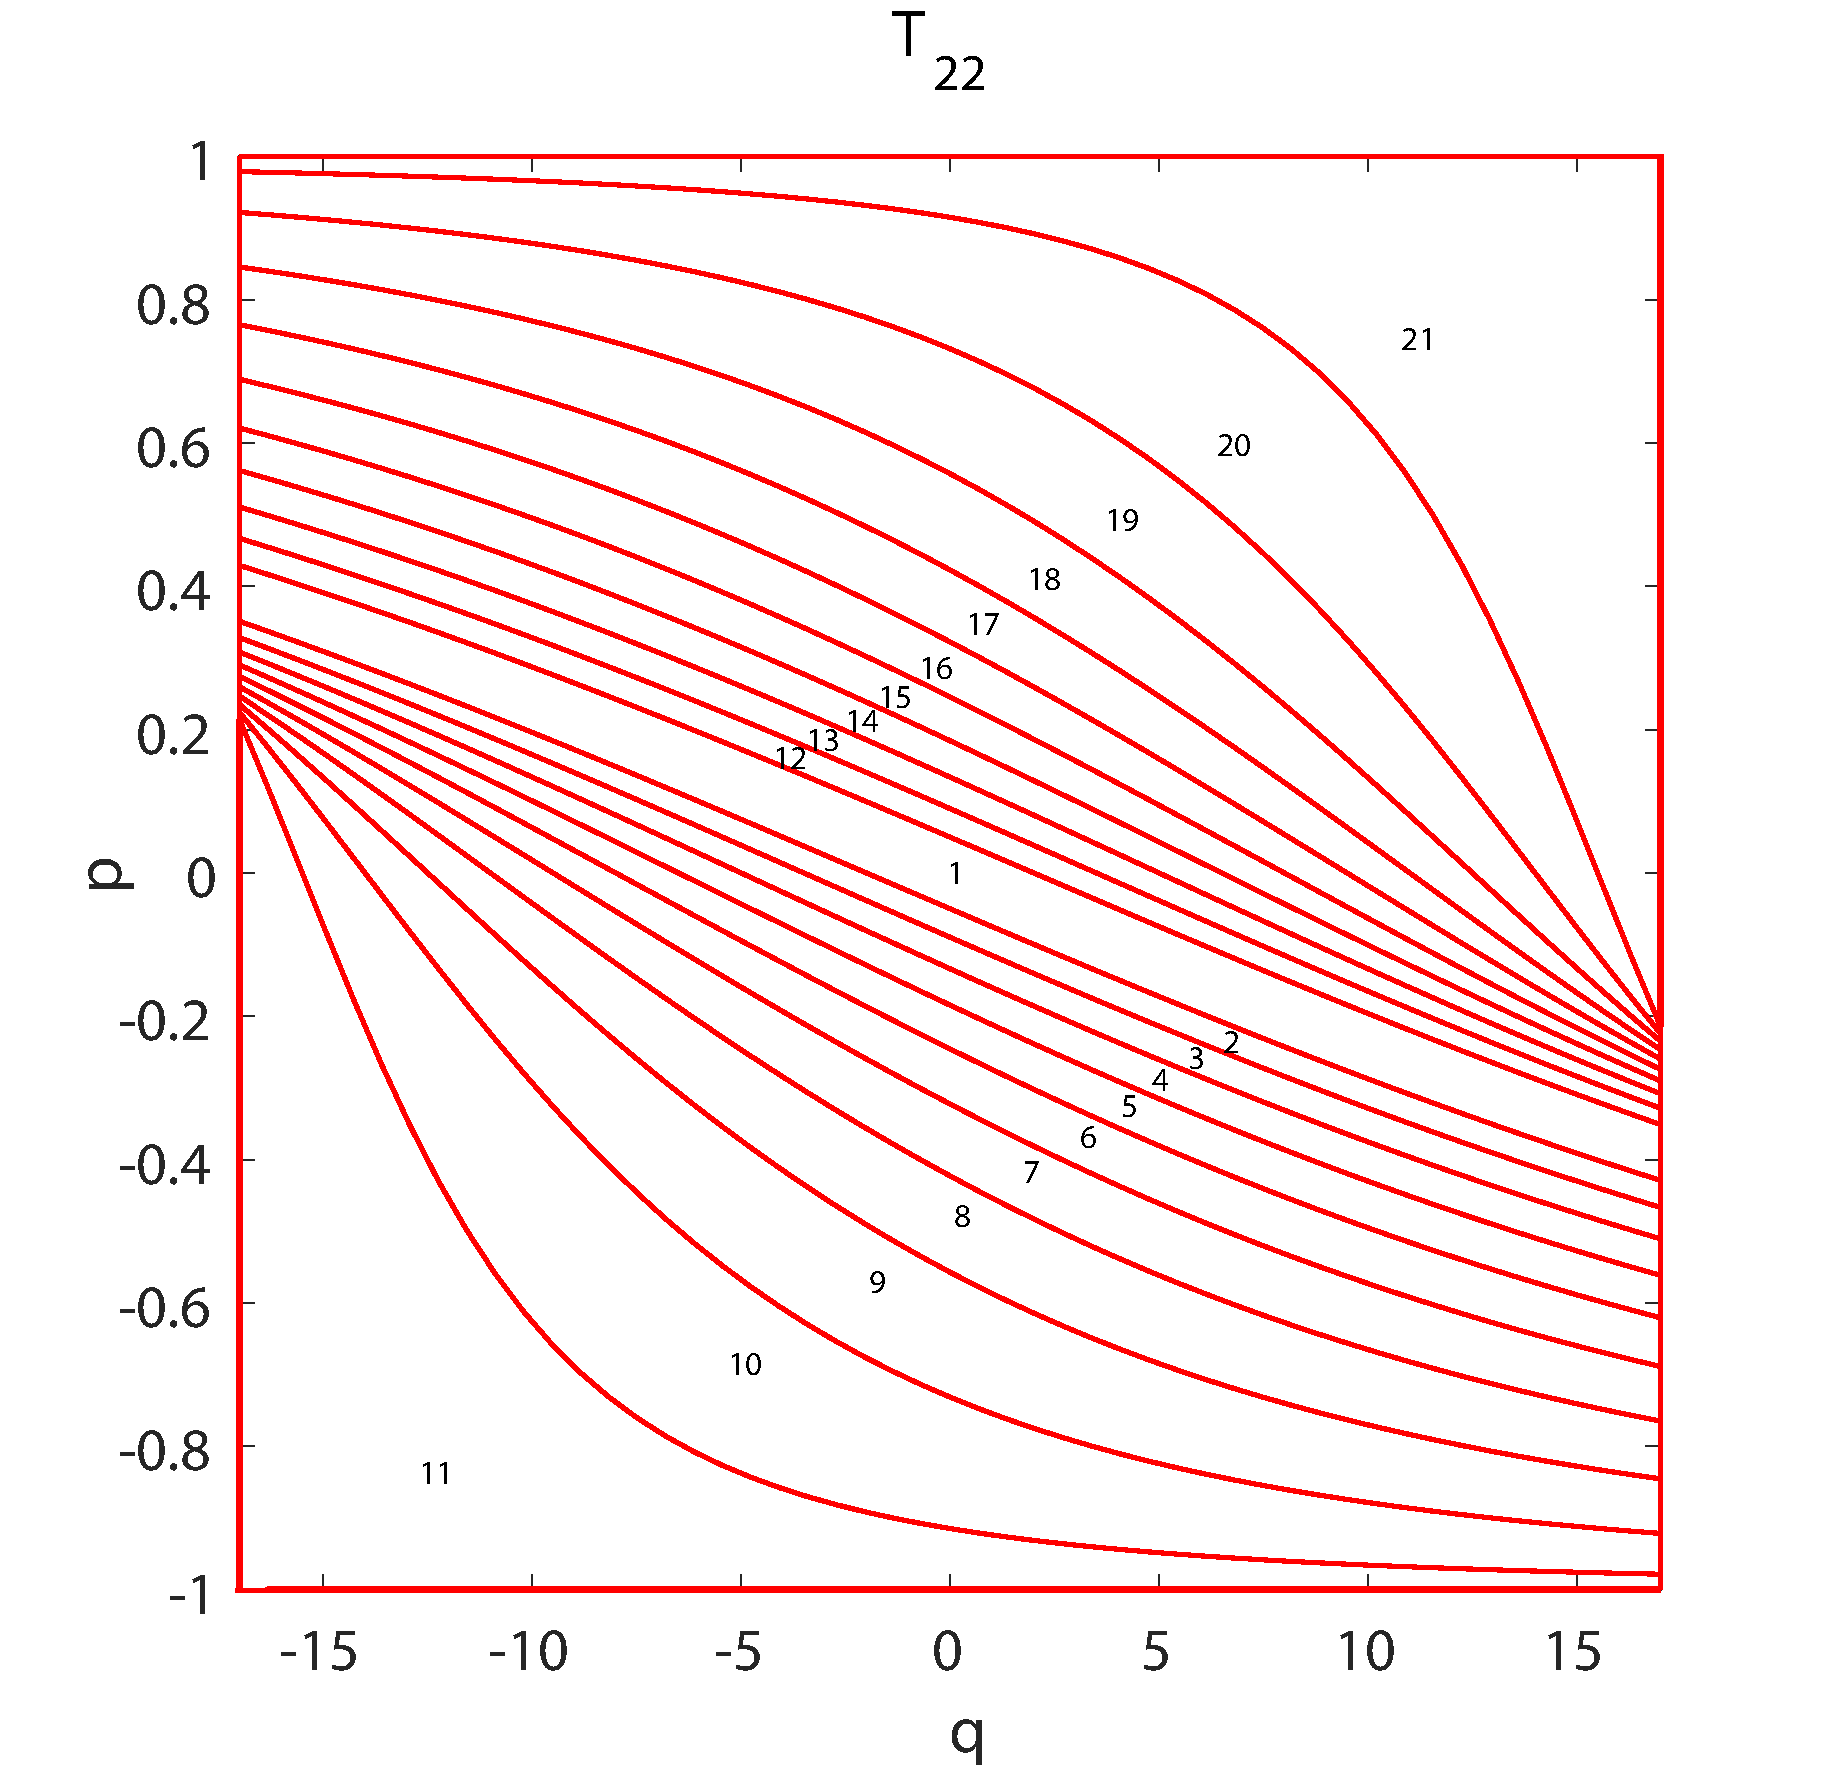
\includegraphics[width = 0.7\textwidth]{target10facetedcup1}
\caption{\textbf{Target PS of the $20$-faceted cup.}
The red lines are the boundaries $(\partial\mbox{\set{T}{$22$,}{\lineak}})_{\lineak=1, \cdots, 21}$ which are determined analytically. The numbers inside the regions \set{T}{$22$,}{\lineak} indicate the value of the index \lineak.}
\label{fig:T20}
\end{figure}
All the possible paths that the rays can follow when propagating within the $20$-faceted cup are determined using the same algorithm developed for the two-faceted cup and explained in Section \ref{sec:algorithm_raymapping}.
 As the number of optical lines increases, the number of possible paths increases as well.
 Therefore, we have to construct a more complicated tree than the one in Figure \ref{fig:tree}.
Despite this, the algorithm explained in the previous section still works fine and, also for the multi-faceted cup we are able to determine all the possible paths $\Pi$ and all the positive luminance regions \set{R}{}{}$(\Pi)$ at target PS.
% \insieme{T}$_{\nline}$.
For a given direction $\variabile{p}=\mbox{const}$ the position coordinates $\variabile{q}^\textrm{\,min}(\Pi,\variabile{p})$ and $\variabile{q}^\textrm{\,max}(\Pi,\variabile{p})$ of the intersection points between the boundaries $ \partial$\set{R}{}{}($\Pi$) and the line $\variabile{p}= \mbox{const}$ are calculated for every possible path $\Pi$. Finally, the target intensity $\hat{I}_{\textrm{PS}}(\variabile{p})$ along the direction $\variabile{p}$ is obtained.
Numerical results for a $20$-faceted cup are given in the next section.
\section{Numerical results for the $20$-faceted cup}
\label{sec:Numerical results_10cup}
In this section the results for the $20$-faceted cup are presented.
We compute the target intensity both with the backward ray mapping method and MC ray tracing.
The same partitioning $P$ of the interval $[-1,1]$ used for the two-faceted cup is considered. A comparison between the reference intensity $\hat{I}_{\textrm{ref}}$ and the ray mapping intensity $\hat{I}_{\textrm{PS}}$ is shown in Figure \ref{fig:intensity10cup}, where $\hat{I}_{\textrm{ref}}$ is obtained using QMC ray tracing with $10^8$ rays.
\begin{figure}[h!]
\centering
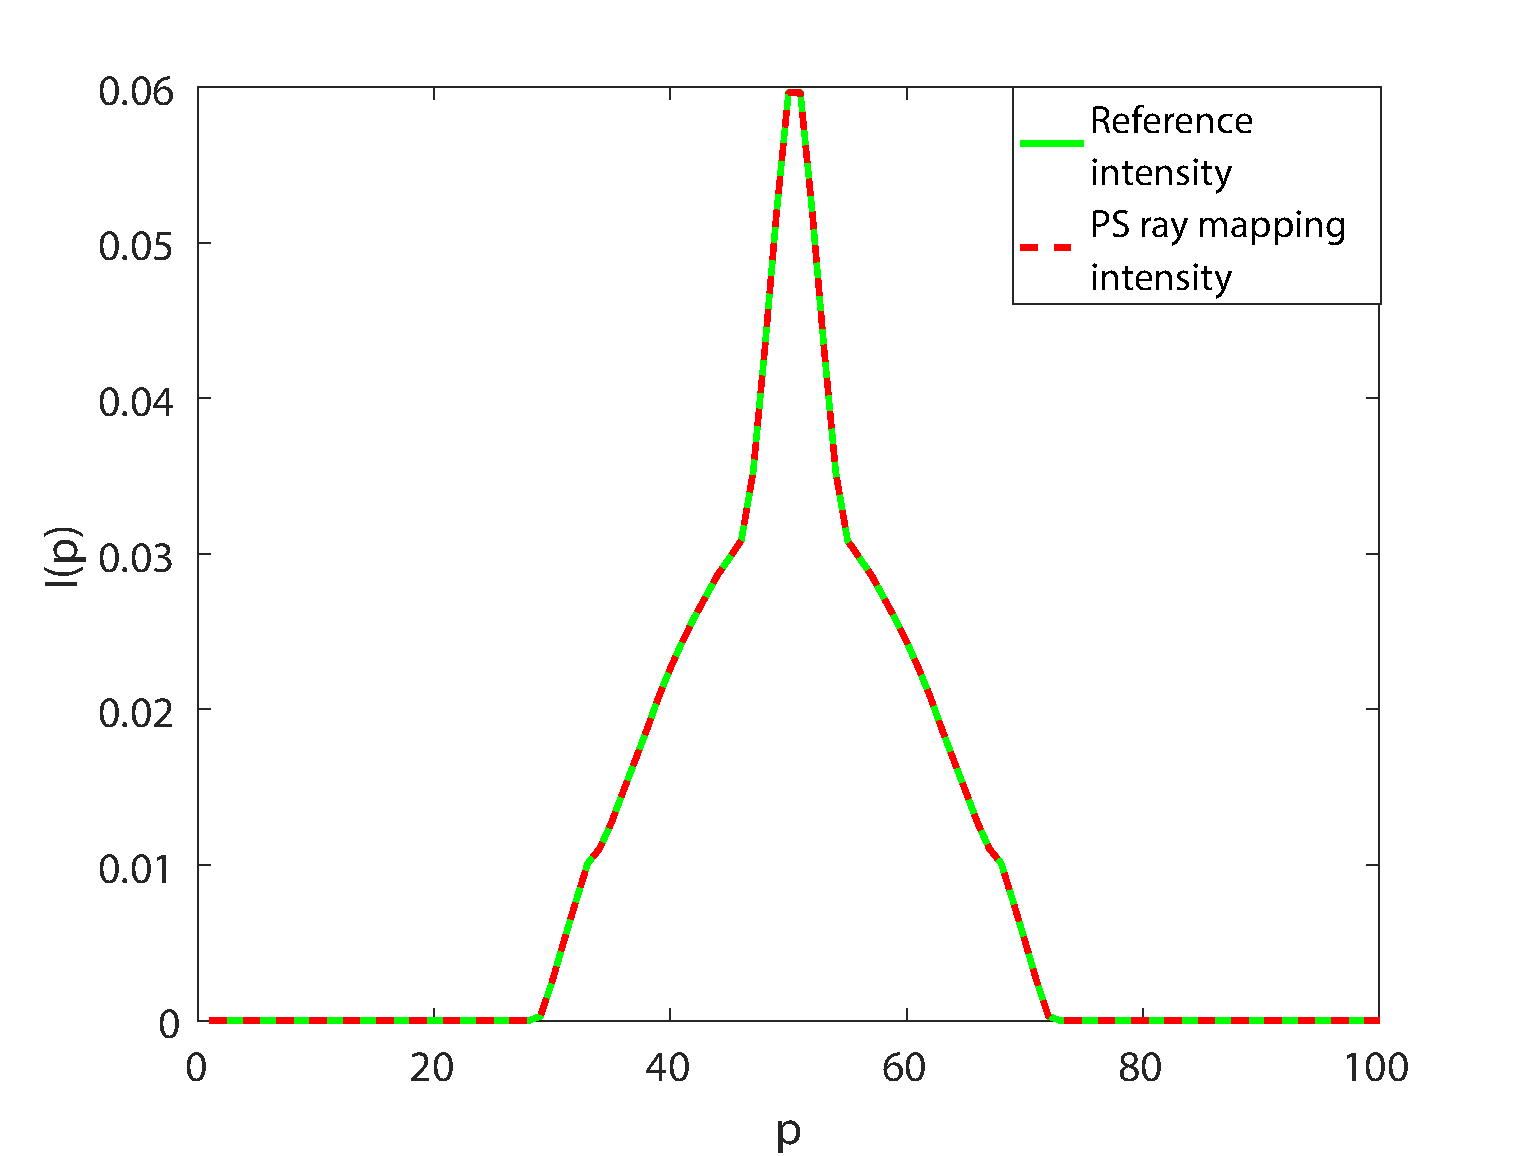
\includegraphics[width = 0.7\textwidth]{intensity_10_cup_raymapping}
\caption{\textbf{Intensity for the $20$-faceted cup}.
Comparison between the reference intensity (QMC ray tracing with $10^8$ rays) and the ray mapping intensity.}
\label{fig:intensity10cup}
\end{figure}
\begin{figure}[h!]
\centering
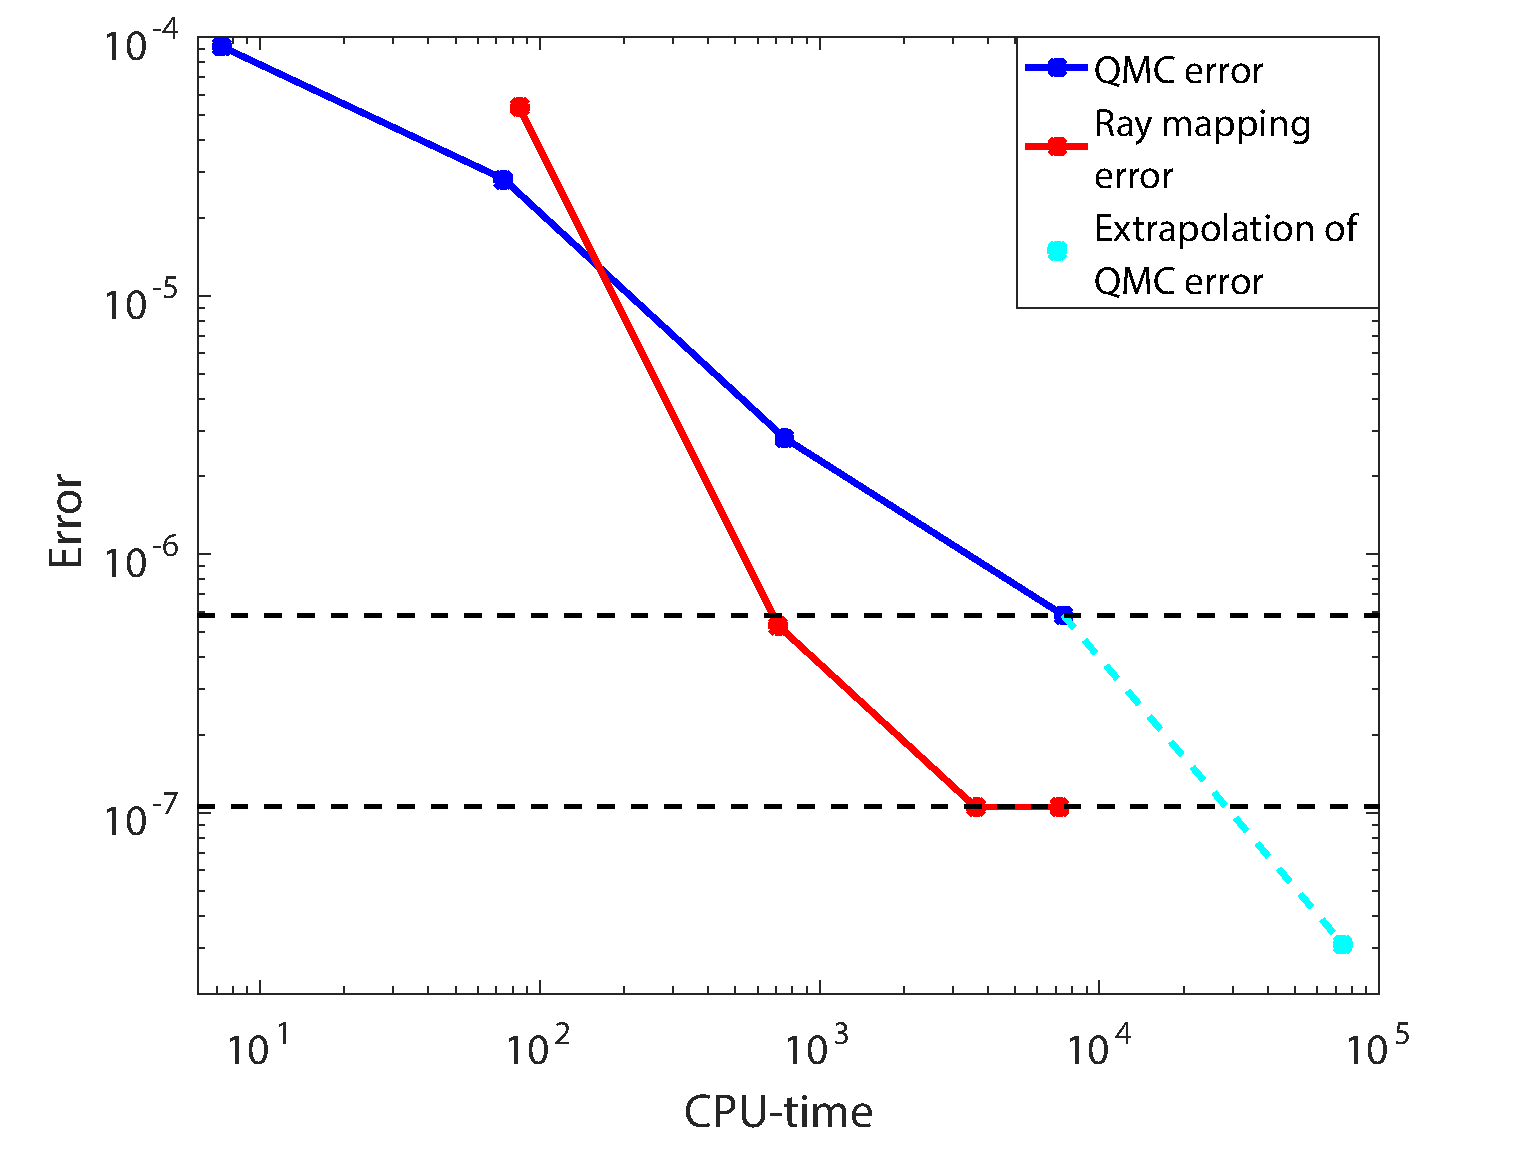
\includegraphics[scale=.4]{error_10_cup_raymapping}
\caption{\textbf{Errors for the $20$-faceted cup as a function of the CPU-time.} The ray mapping method is more accurate than QMC ray tracing and it is faster in case an error smaller than $10^{-5}$ is desired.}
\label{fig:error10cup} 
\end{figure}
\\ \indent Note that the intensity profile in Figure \ref{fig:intensity10cup} is more concentrated around the direction $\variabile{p}=0$ than the intensity of the two-faceted cup (see Figure \ref{fig:intensity_cup}). In particular, increasing the number of left and right reflectors the intensity profile becomes more and more peaked around the center approaching the profile of a parabolic reflector, (see Chapter \ref{chap:triangulation}).
The error between the approximate intensities $\hat{I}_{\textrm{A}}$ ($\textrm{A} = \textrm{QMC}, \textrm{PS}$) and the reference intensity $\hat{I}_{\textrm{ref}}$ is shown in Figure \ref{fig:error10cup}. 
The PS intensity is calculated using (\ref{eq:normalized_PS_intensity}) where the integral is approximated using the trapezoidal rule. Figure \ref{fig:error10cup} shows that increasing the number of intervals in the trapezoidal rule, the PS error decreases. We computed the PS error four times considering $1, 10, 50$, and $100$ intervals in the trapezoidal rule. 
We remark that the PS method gives the value of the intensity pointwise, therefore we can compute the PS intensity without numerical integration. Nevertheless, we calculate the averaged intensity because we want to compare it with the QMC intensity $\hat{I}_{\textrm{QMC}}$.
\\ \indent The error convergence is depicted in Figure \ref{fig:error10cup} with the red line.
Since all the boundaries of the regions in PS are calculated exactly, our expectation is that the PS intensity is the exact intensity.
From Figure \ref{fig:error10cup} we observe that the minimum ray mapping error has an order of magnitude of $10^{-7}$.
This is due to the fact that for the $20$-faceted cup the intensity cannot be computed exactly. 
Therefore, we took as reference intensity $\hat{I}_{\textrm{ref}}$ an intensity computed with QMC ray tracing using $10^8$ rays which is not the exact intensity.
The error between the normalized exact intensity $\hat{I}_{\textrm{exact}}$ and the normalized approximate intensity $\hat{I}_{\textrm{A}}$ is given by:
\begin{equation}\label{eq:qmc_error_20_cup}
\frac{1}{\textrm{Nb}}\sum_{\variabile{h} = 1}^{\textrm{Nb}}| \hat{I}_{\textrm{exact}}(\variabile{p}^\variabile{h}) - \hat{I}_{\textrm{A}}(\variabile{p}^\variabile{h})| \leq
\frac{1}{\textrm{Nb}}\Bigg(\sum_{\variabile{h} = 1}^{\textrm{Nb}}\big| \hat{I}_{\textrm{exact}}(\variabile{p}^\variabile{h}) - \hat{I}_{\textrm{ref}}(\variabile{p}^\variabile{h})\big| +
\sum_{\variabile{h} = 1}^{\textrm{Nb}}\big| \hat{I}_{\textrm{ref}}(\variabile{p}^\variabile{h}) - \hat{I}_{\textrm{A}}(\variabile{p}^\variabile{h})\big|\Bigg)\,.
\end{equation}
To give an estimation of the first term on the right hand side of (\ref{eq:qmc_error_20_cup}), we do a linear extrapolation from the errors values obtained. The extrapolated point at the time needed for computing the reference intensity (cyan dot in Figure \ref{fig:error10cup}) gives an estimation of the error between the reference intensity and the exact intensity. If the reference intensity is \textit{exact} then we would expect an error \textit{exactly} equal to $0$.
From the extrapolation we obtain
\begin{equation*}\sum_{\variabile{h} = 1}^{\textrm{Nb}}| \hat{I}_{\textrm{exact}}(\variabile{p}^\variabile{h}) - \hat{I}_{\textrm{ref}}(\variabile{p}^\variabile{h})|/\textrm{Nb}\approx 1.02*10^{-7}. \end{equation*}
The results show that 
\begin{equation*}
\sum_{\variabile{h} = 1}^{\textrm{Nb}}| \hat{I}_{\textrm{exact}}(\variabile{p}^\variabile{h}) - \hat{I}_{\textrm{ref}}(\variabile{p}^\variabile{h})|/\nbin
\approx \sum_{\variabile{h} = 1}^{\nbin}|\hat{I}_{\textrm{ref}}(\variabile{p}^\variabile{h}) - \hat{I}_{\textrm{PS}}(\variabile{p}^\variabile{h})|/\nbin.
\end{equation*}
Since the accuracy of the reference intensity is comparable with the accuracy of the PS intensity, we claim that the error found with backward ray mapping is also due to the QMC error. We expect that considering a more accurate reference intensity, obtained for instance using QMC ray tracing with more rays, the PS error would decrease.
We conclude that the backward ray mapping method performs very well also for more complicated systems.
Compared to QMC ray tracing the new method is not only faster but also much more accurate.
\section{Discussions}
In this chapter, we presented an backward ray mapping method to compute the target intensity of a given optical system.
The method employs the PS of \textit{all} the lines that form the system.
All these phase spaces are related to each other through two different kind of maps.
A concatenation of these two maps gives a map that connects the coordinates of the rays at the source with those at the target.
Employing the inverse of the concatenated map, all the possible paths that rays can follow during their propagation are found. 
Only the rays located on the boundaries of the positive luminance regions are traced,
where every region is formed by rays that follow the same path during their propagation. From those rays the output intensity is calculated. \\ \indent
We presented numerical results for two optical systems: the two-faceted cup and the $20$-faceted cup. The boundaries of the regions that form every PS are determined exactly.
 Numerical results show that the exact output intensity is obtained.
 We compared our method with MC and QMC ray tracing showing significant advantages in terms of the accuracy and the computational time.
 We conclude that the ray mapping method applied to systems formed by straight line segments calculates the \textit{exact} intensity.\\
\indent In the next chapter we present the method extended to systems formed by curved lines. 


